\chapter{Stellar Kinematics and Populations}
	\label{cha:stellar}
With the advent of integral-field spectroscopy (IFS), we can now observe the spatially-resolved properties of a galaxy without relying on extrapolations of or multiple observations with slits. Surveys such as the Spectrographic Areal Unit for Research on Optical Nebulae (SAURON; \citealt{deZeeuw2002}) and Atlas$^\text{3D}$ \citep{Cappellari2011} have demonstrated that systematic IFS surveys provide a wealth of information about the structure of nearby galaxies. This chapter focuses on the resolved stellar properties of our sample of radio galaxies. In this we aim to demonstrate that our radio selected sample is no different in the $V$-band than optically-selected early-type galaxies ETGs from the MASSIVE (not an acronym; \citealt{Ma2014}) and Atlas$^\text{3D}$ samples. We achieve this by showing that they are consistent with the defining characteristics of ETGs that are accessible to $V$-band IFS data. These characteristics are (with relevant section is shown in parentheses): regular/non-regular rotator classification scheme, qualitative kinematic classes (see Fig.\,\ref{fig:EgSubstructure}; Section \ref{subsec:maps}), fast/slow rotator classifications (\ref{subsec:FSRot}), radially resolved specific angular momentum profiles (with $\lambda_R$; \ref{subsec:ResolvedLambda_R}), absorption line strengths(\ref{subsec:absorption}), Mg\,--\,$\sigma$ relation (\ref{subsubssec:Mgsigma}), stellar populations (\ref{subsec:ssp}) and their gradients (\ref{subsubsec:popGrad}) and the kinematically-decoupled core (KDC) age\,--\,size relation(\ref{subsec:popKDC}). 

The chapter is structured as follows: firstly we present the kinematic maps for the stellar component of each galaxy (section \ref{sec:stellarKin}) and the distribution of the sample on the $\lambda_\mathrm{R_e}$\,--\,ellipticity diagram. Then, in section \ref{sec:pop}, we investigate the stellar populations of each galaxy using the measured absorption line strengths, looking for atypical ETGs (a typical ETG has old, metal rich, alpha-enhanced stellar populations with virtually no radial gradients). Finally, in Section \ref{sec:stellarDiscussion} we discuss these observations.


\section{Kinematics}
	\label{sec:stellarKin}

	\subsection{Maps}
		\label{subsec:maps}
		Using the methods described in Chapter \ref{cha:Data} to reduce (see Sections \ref{subsec:VIMOSreduction} and \ref{subsec:MUSEreduction}), spatially bin (Section \ref{subsec:Binning}) and fit the stellar line-of-sight velocity distributions (LOSVDs; here parametrised by the mean velocity, $v$ and velocity dispersion, $\sigma$, only; Section \ref{subsec:StellarFit}), we produce stellar kinematic maps. These kinematic maps are shown in Figs.\,\ref{fig:VIMOS_stellar} and \ref{fig:MUSE_stellar} with their associated uncertainties for the VIMOS and MUSE datacubes, respectively. 

		As part of this project, radio continuum maps have been produced by Robert Laing (private communication) by re-reducing archival data from the Very Large Array (VLA) in a variety of bands. We also use the VLA image from \citet{Lanz2010} for NGC 1316. These images have a variety of resolutions and spatial scales: we choose the image that closest matches our VIMOS and MUSE observations and overlay this on all maps (except those showing uncertainties) in green contours. Additionally, this project has also secured observations of the Southern Sample (except NGC 1316 and NGC 1399 for technique reasons) from the Atacama Large Millimeter/sub-millimeter Array (ALMA). \ce{^{12}CO(2-1)} flux maps have been produced by Ruffa et al.\ (in prep.). These are shown in cyan contours on all maps (except those showing uncertainties). 

		\begin{figure}
			\centering
			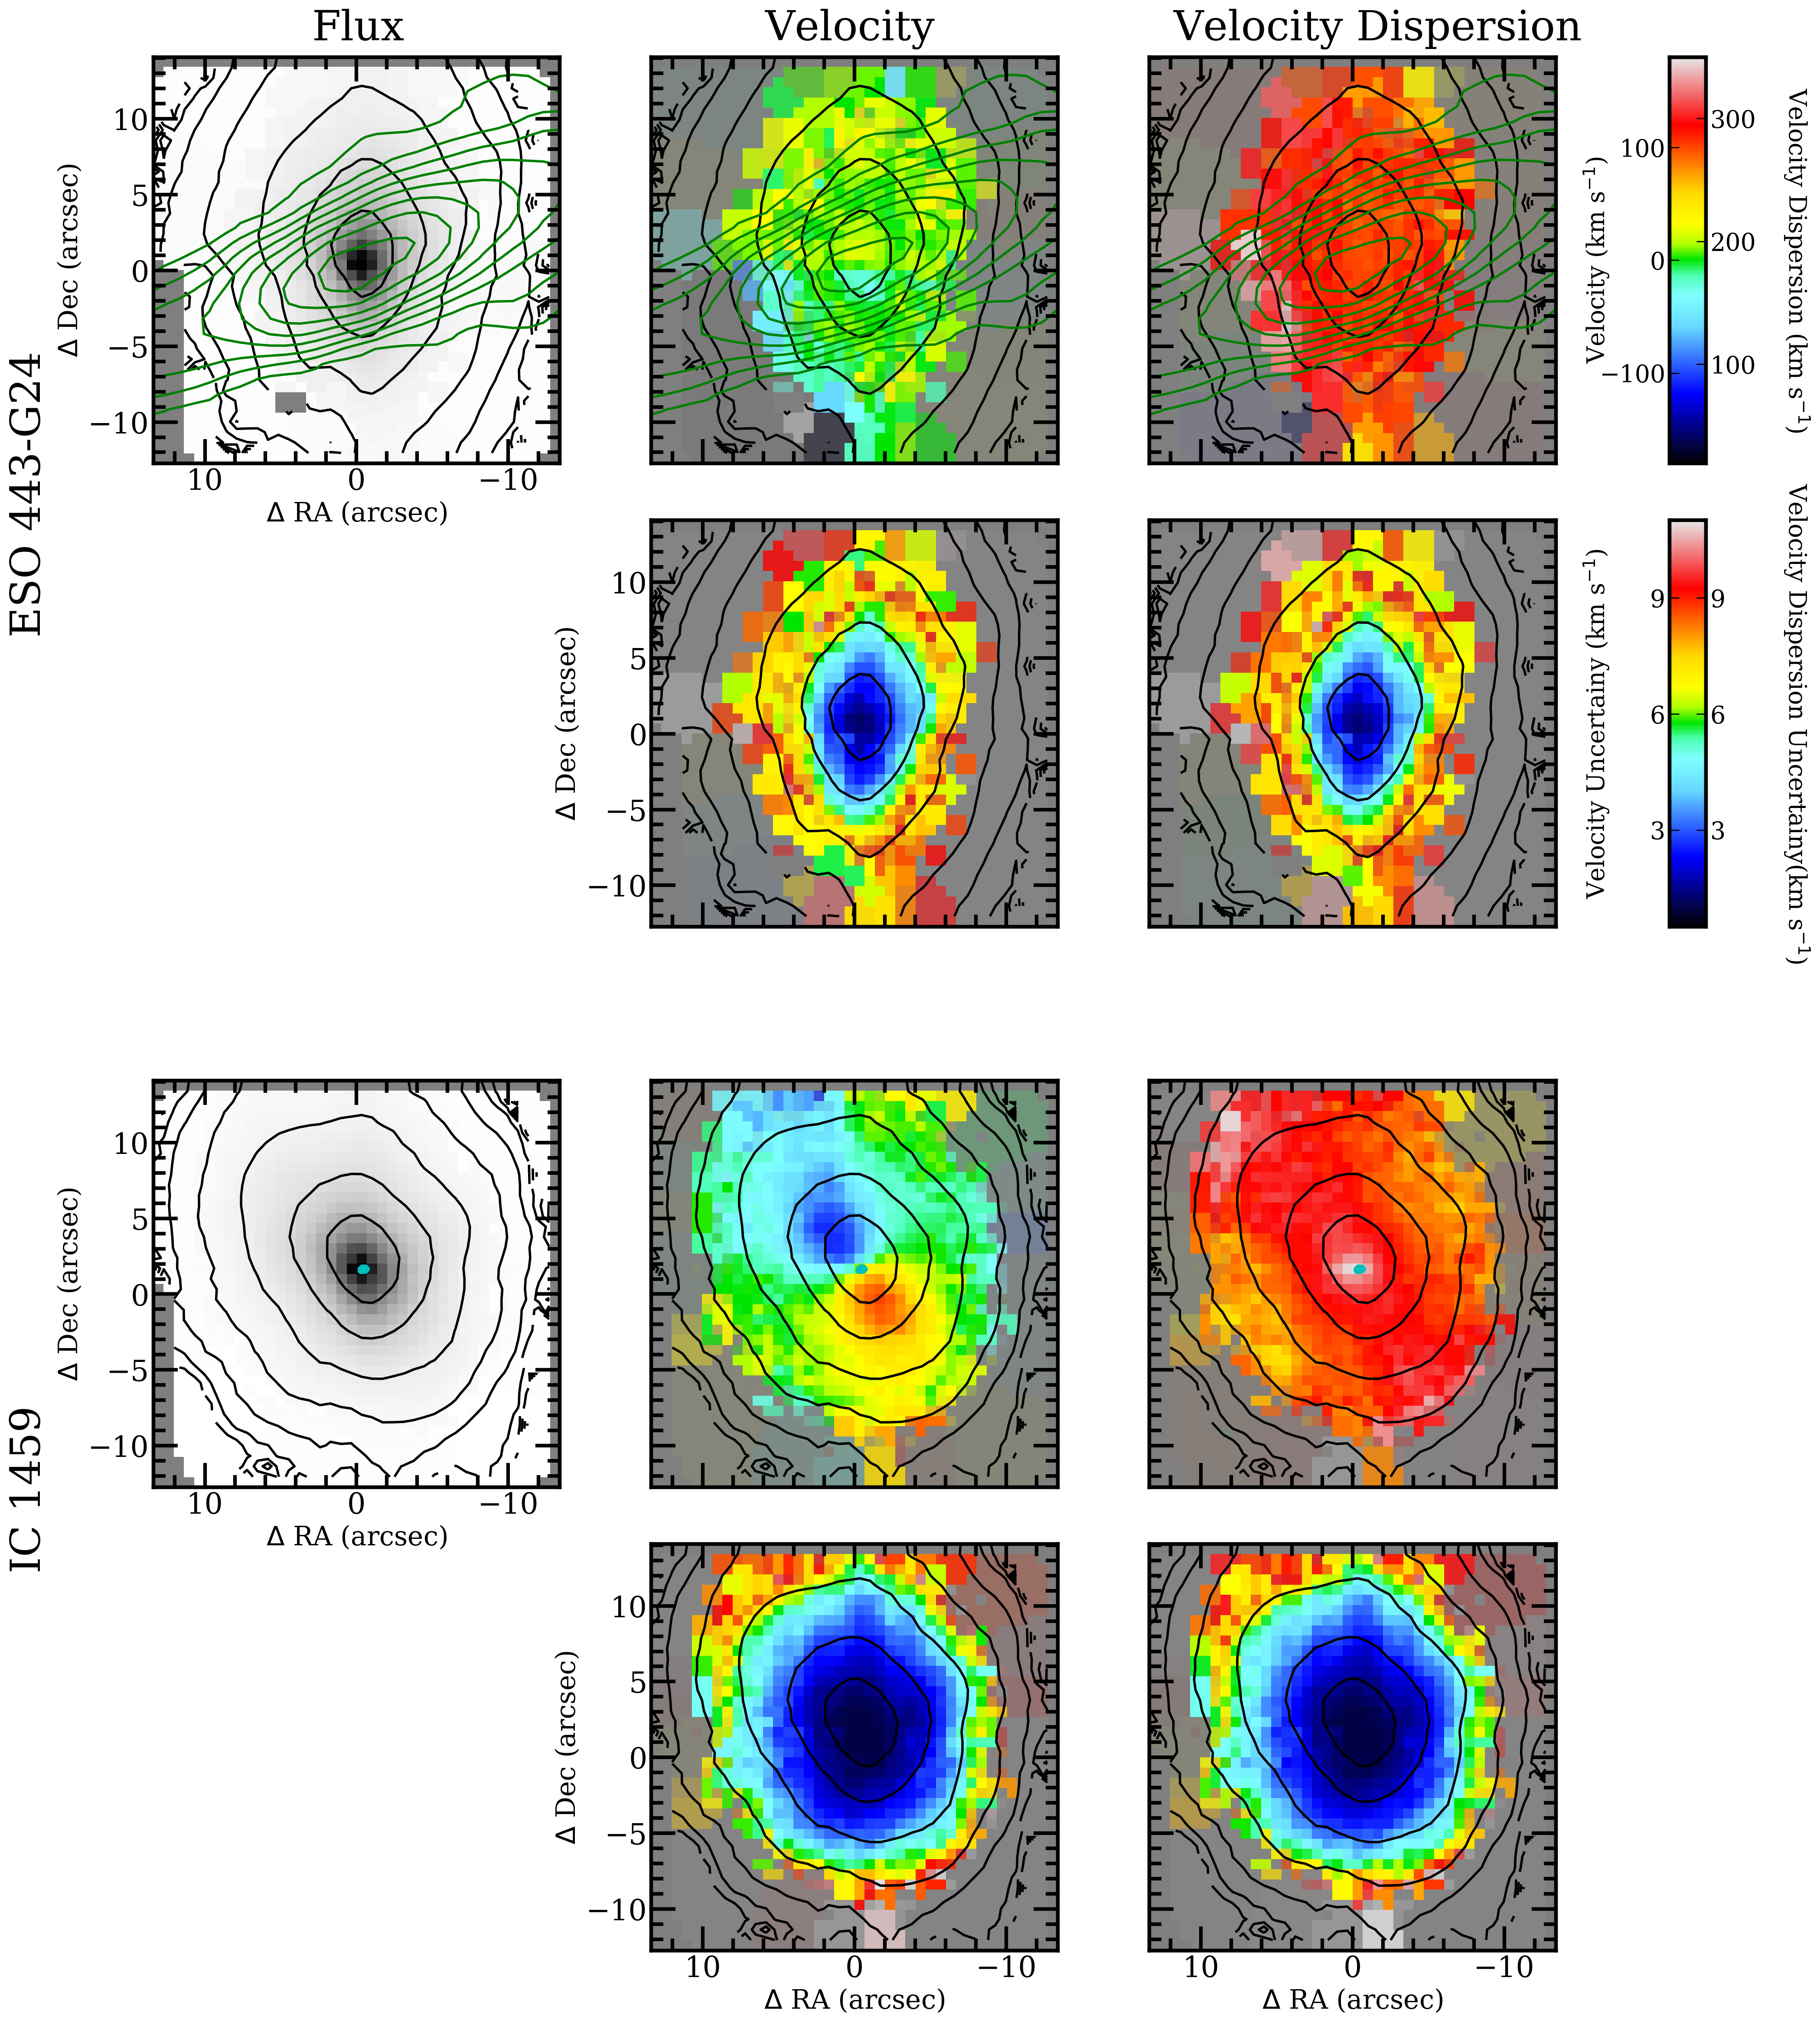
\includegraphics[height=0.62\textheight]{chapter4/vimos/kin1.png}
			\caption[VIMOS stellar kinematic maps]{VIMOS stellar kinematic maps. Left to right: flux (image), mean velocity and velocity dispersion. Top to bottom: ESO 443-G24 and IC 1459. Alternate rows show a given parameter its associated uncertainty. Flux contours (isophotes) are shown in black, \ce{^{12}CO(2-1)} contours from ALMA in cyan and radio continuum contours from VLA in green. The radio band displayed depends on the data available in the archive and which images had a similar resolution and scales. Limits on the colour scale are: mean velocity maps -180 to 180\,$\mathrm{km \, s^{-1}}$, mean velocity uncertainty 1 to 11\,$\mathrm{km \, s^{-1}}$, velocity dispersion 35 to 350\,$\mathrm{km \, s^{-1}}$ and velocity dispersion uncertainty 1 to 11\,$\mathrm{km \, s^{-1}}$.} 
			\label{fig:VIMOS_stellar}
		\end{figure}
		\begin{figure}
			\centering
			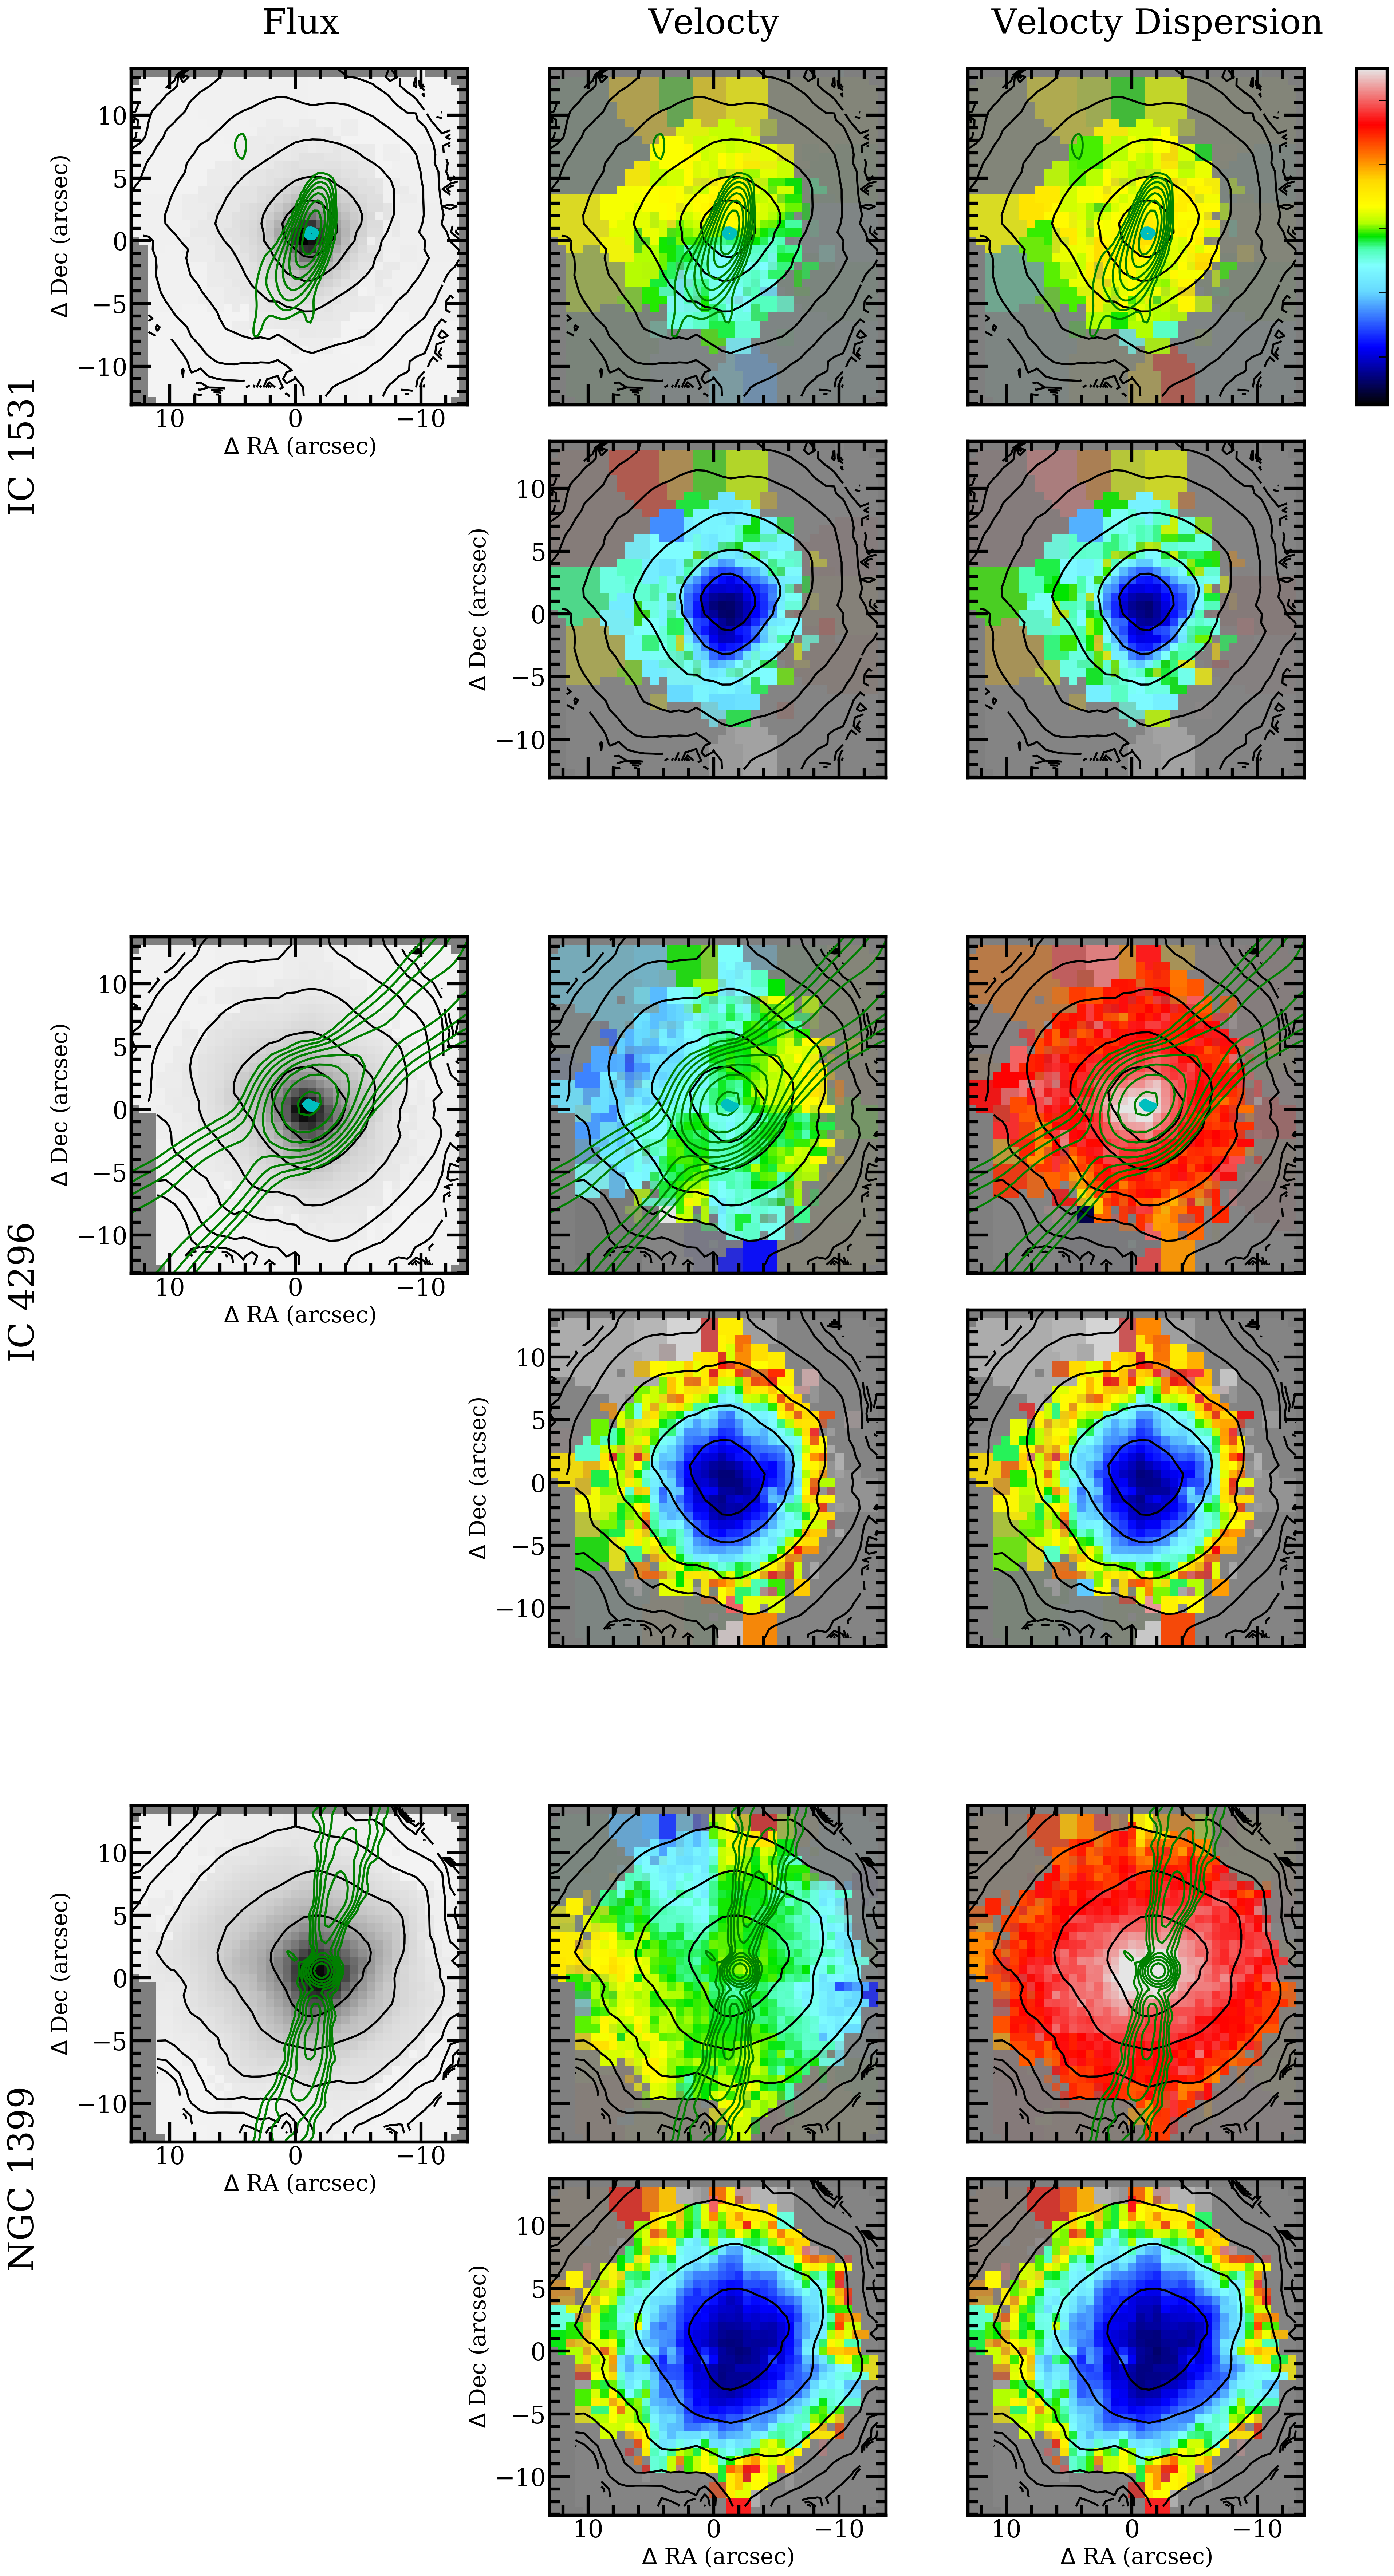
\includegraphics[height=0.94\textheight]{chapter4/vimos/kin2.png}
			\contcaption{\textit{Continued.}}
		\end{figure}
		\begin{figure}
			\centering
			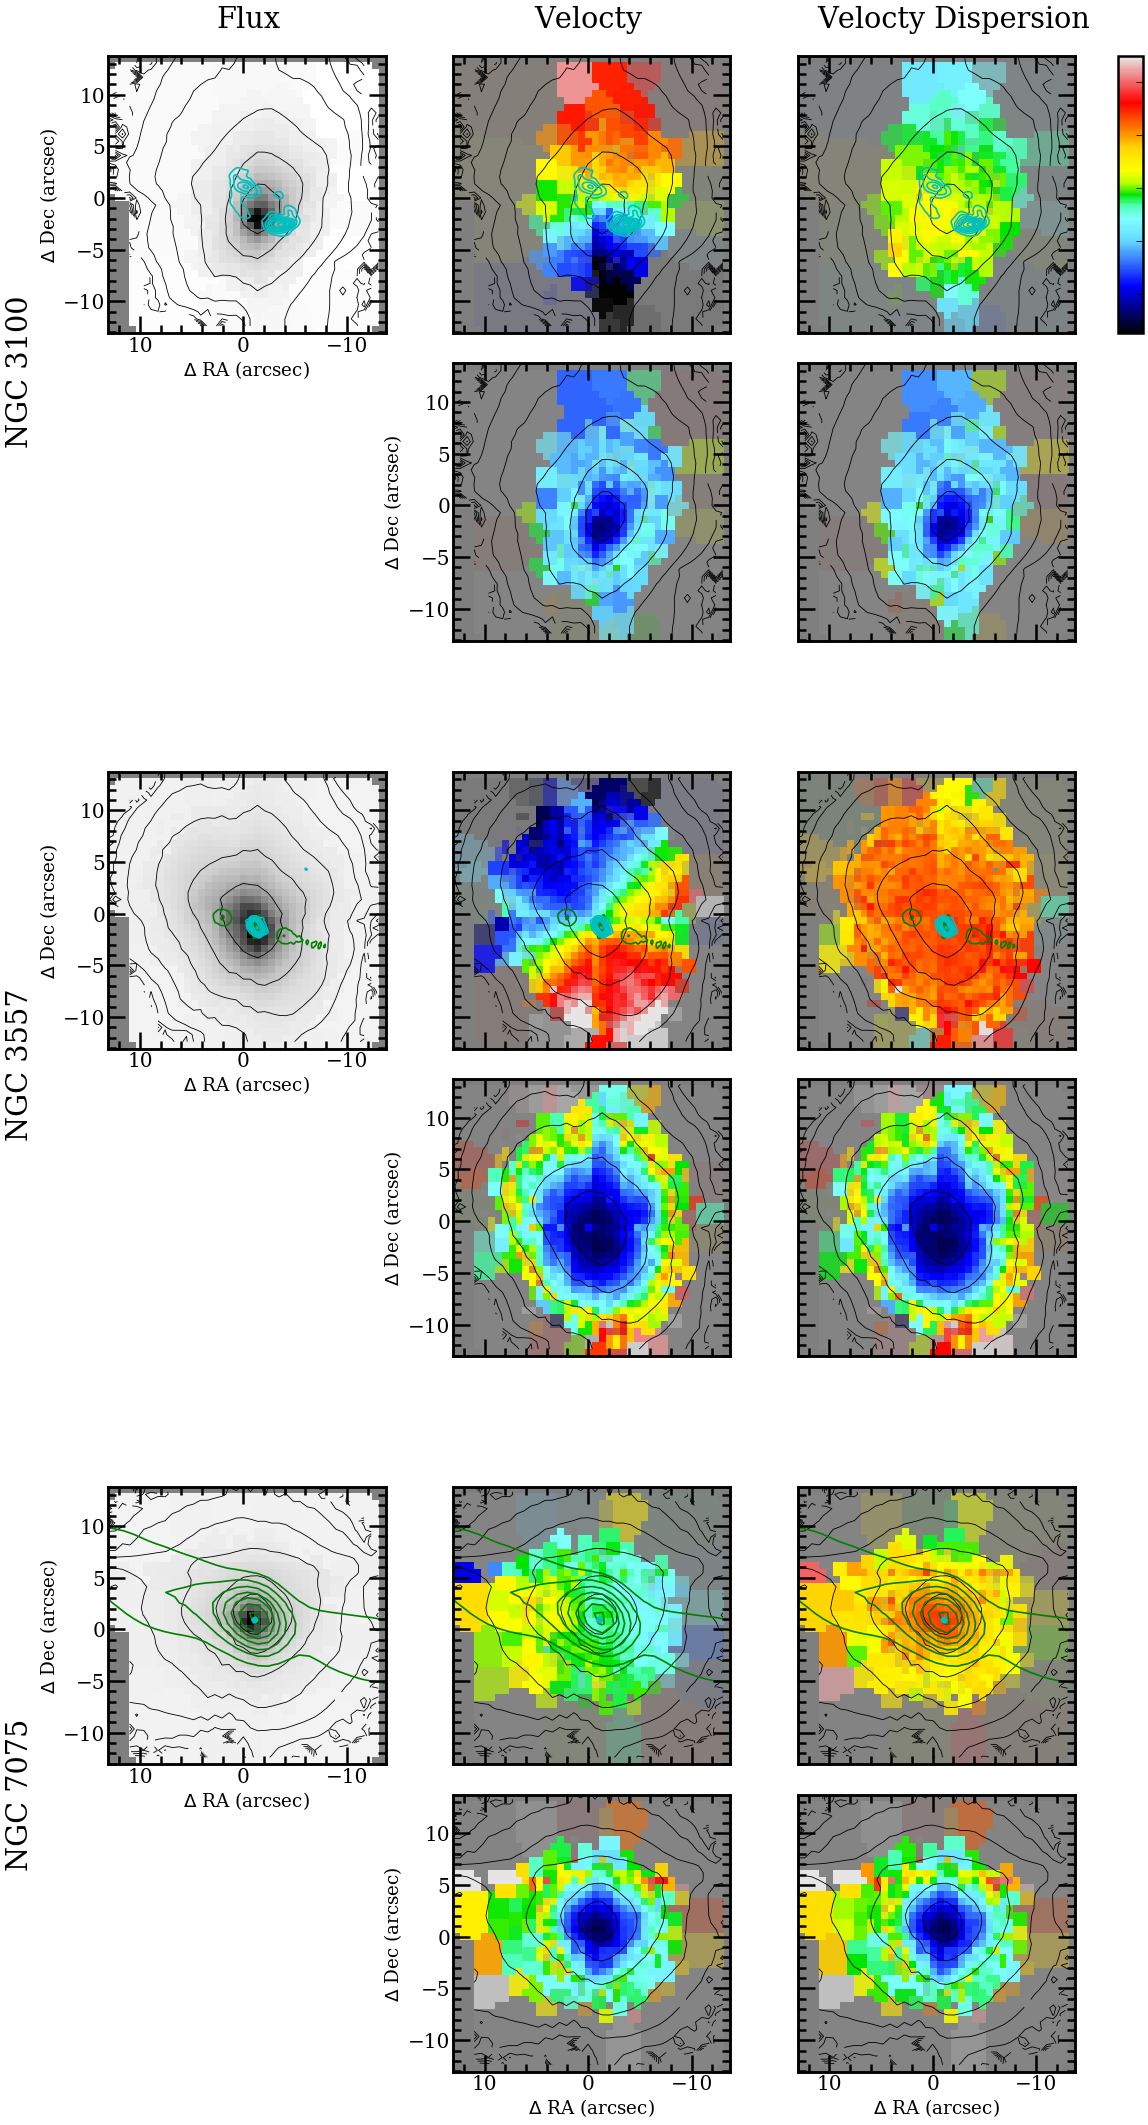
\includegraphics[height=0.94\textheight]{chapter4/vimos/kin3.png}
			\contcaption{\textit{Continued.}}
		\end{figure}
		\begin{figure}
			\centering
			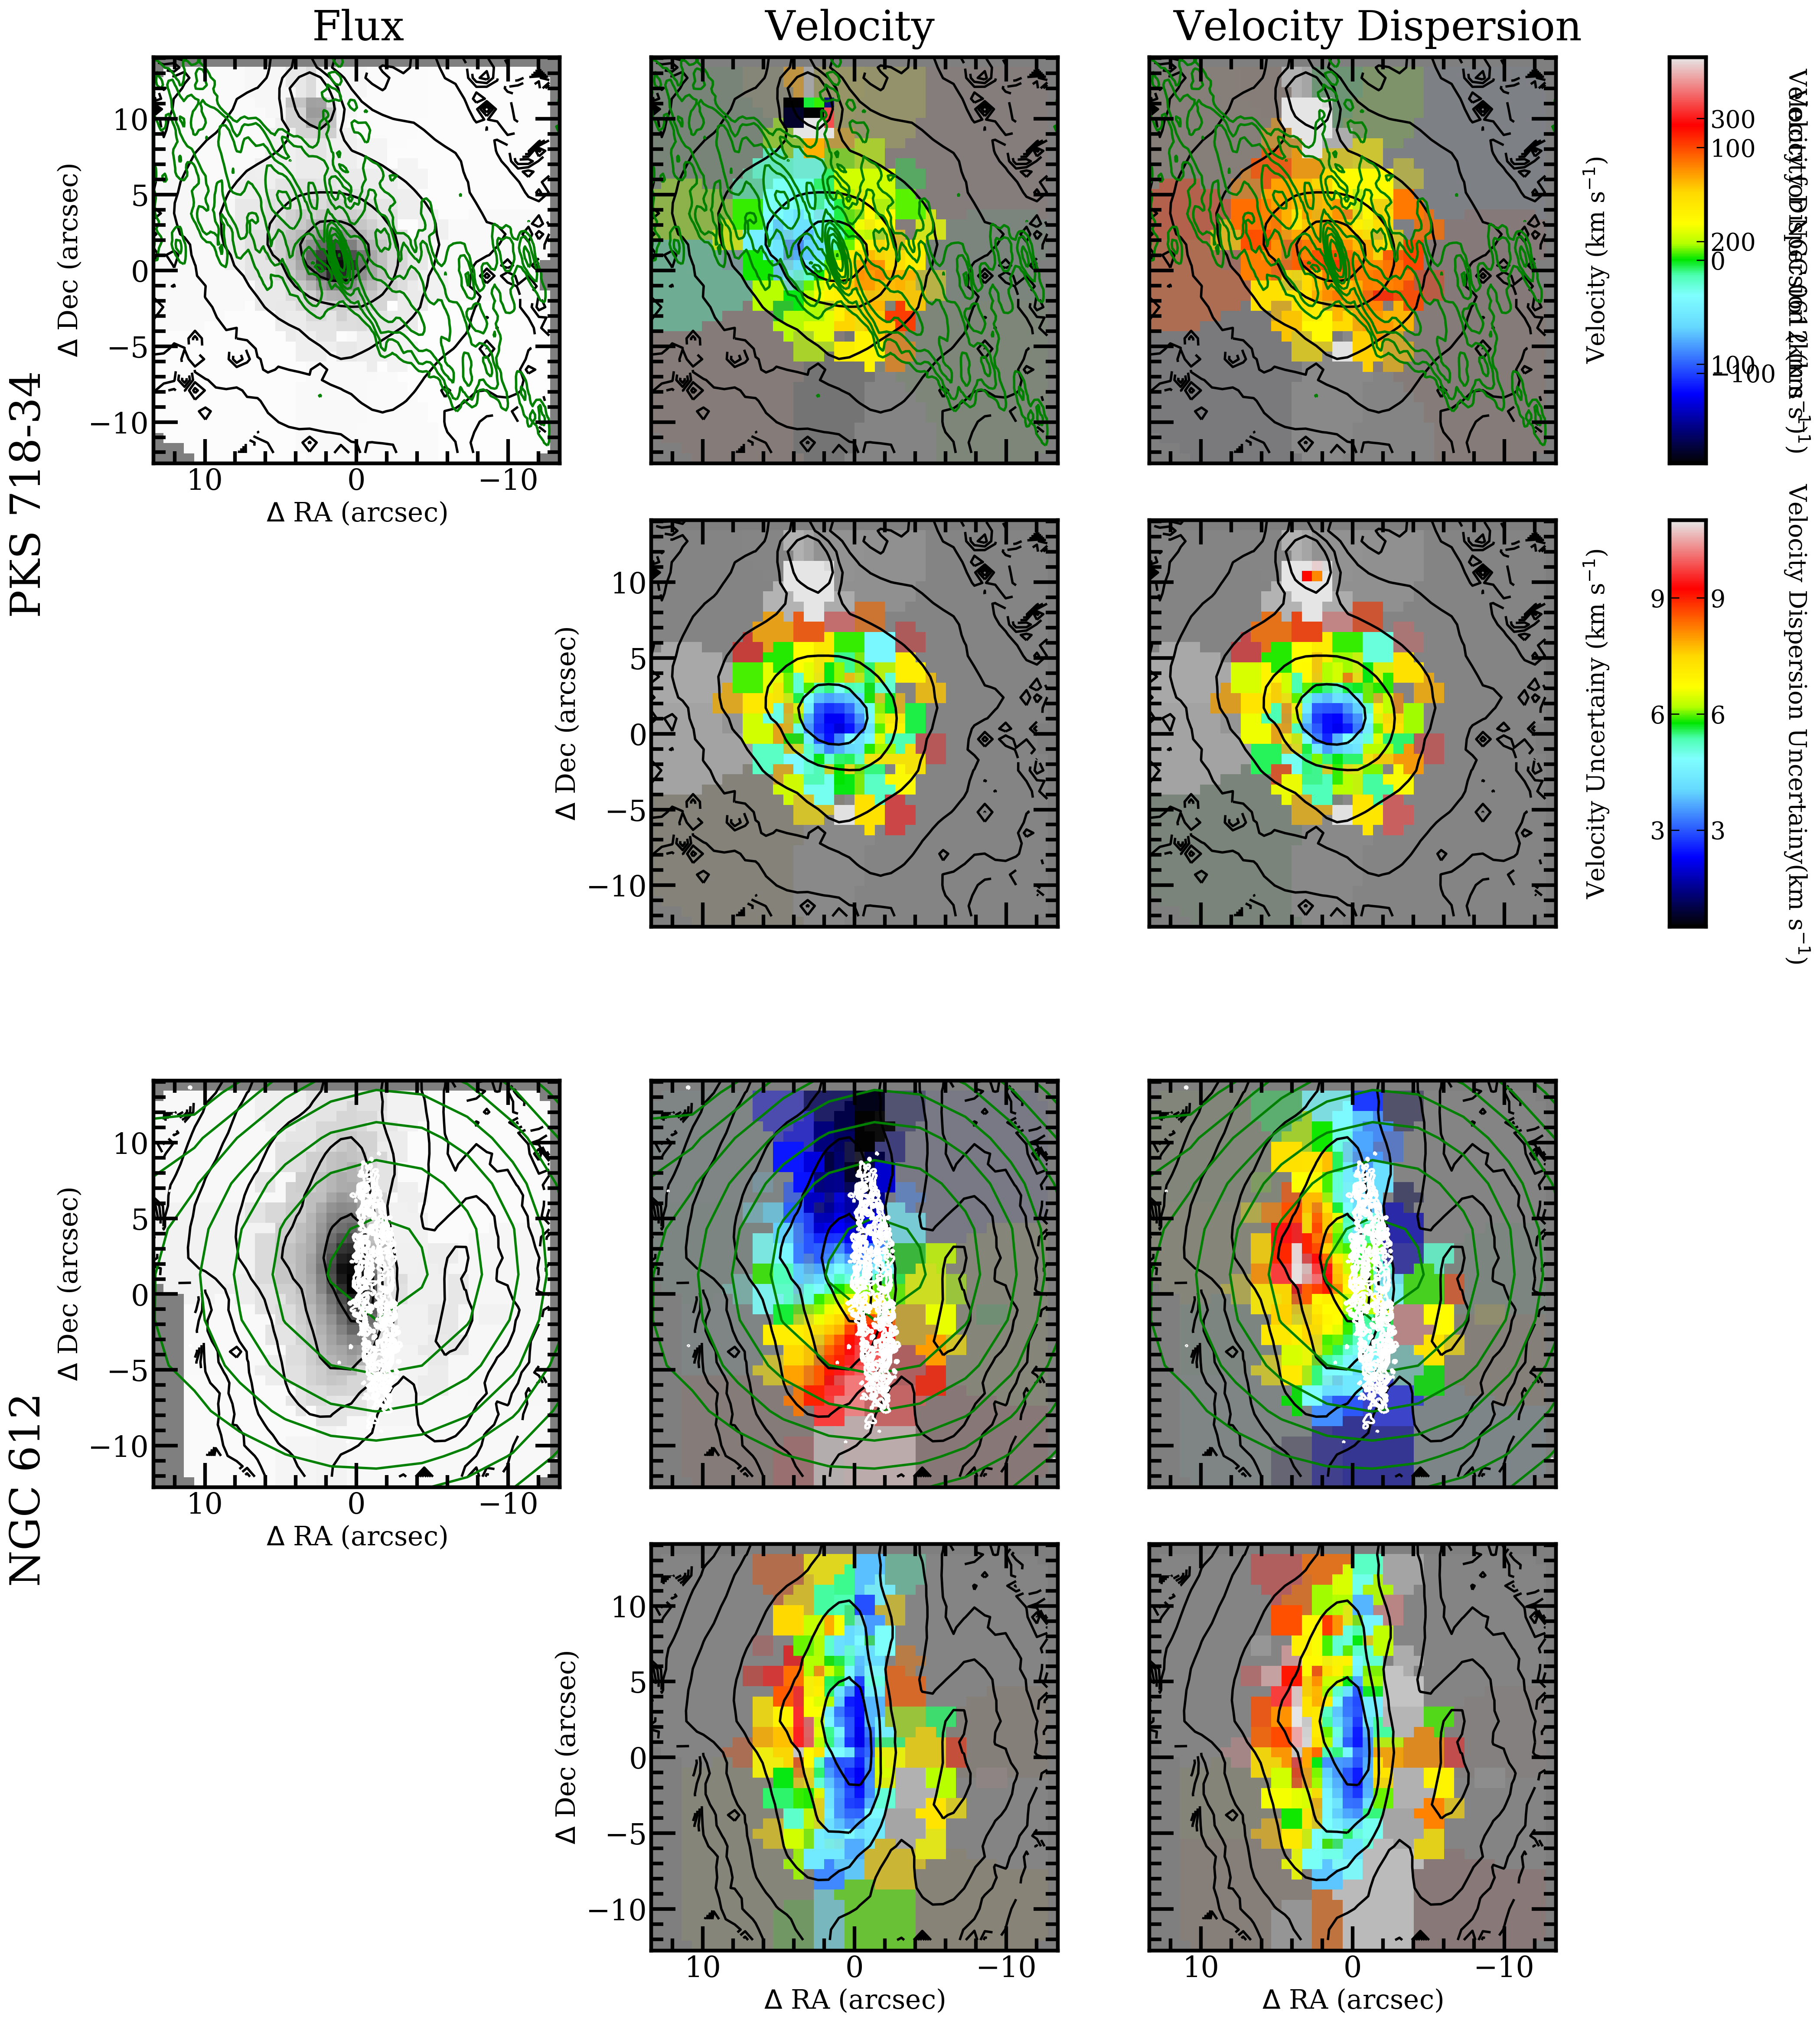
\includegraphics[height=0.62\textheight]{chapter4/vimos/kin4.png}
			\contcaption{\textit{Continued.} The colour scale for the mean velocity map of NGC 612 only is $-322$ to $322 \, \mathrm{km \, s^{-1}}$.}
		\end{figure}

		\begin{figure}
			\centering
			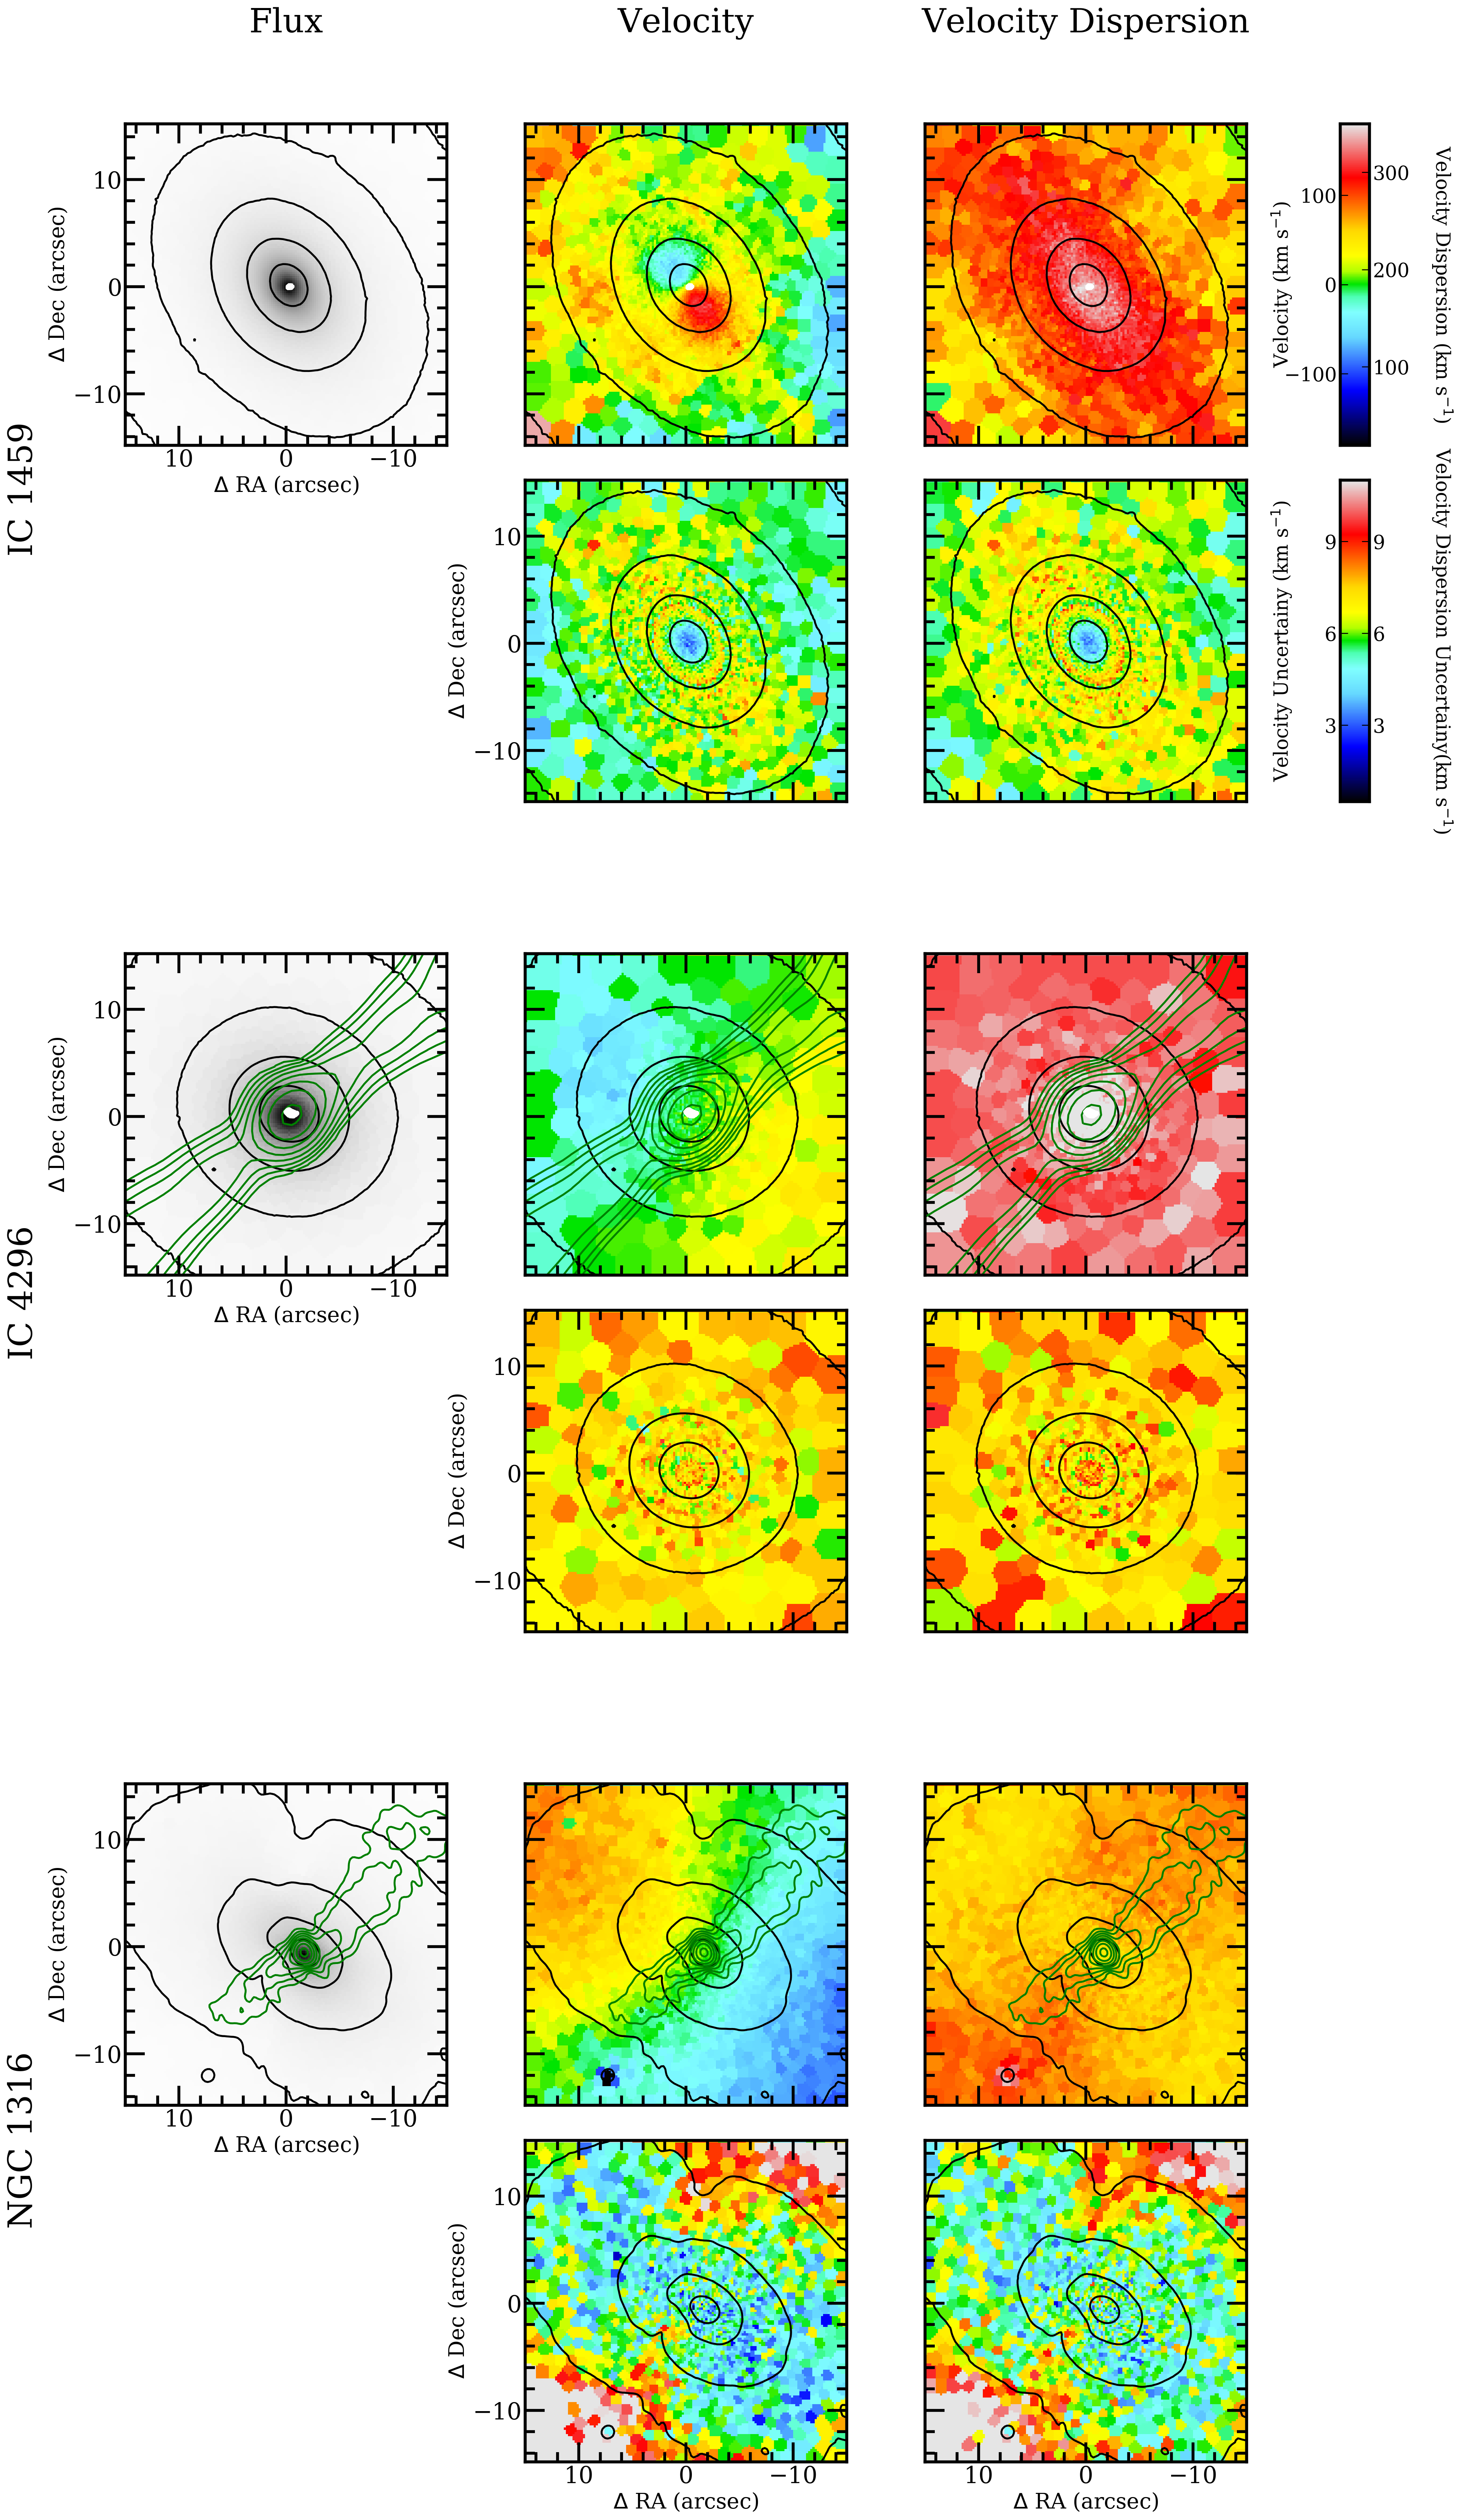
\includegraphics[height=0.94\textheight]{chapter4/muse/kin1.png}
			\caption[MUSE stellar kinematic maps]{As in Figure \ref{fig:VIMOS_stellar} but for the MUSE stellar kinematic maps.}
			\label{fig:MUSE_stellar}
		\end{figure}
		\begin{figure}
			\centering
			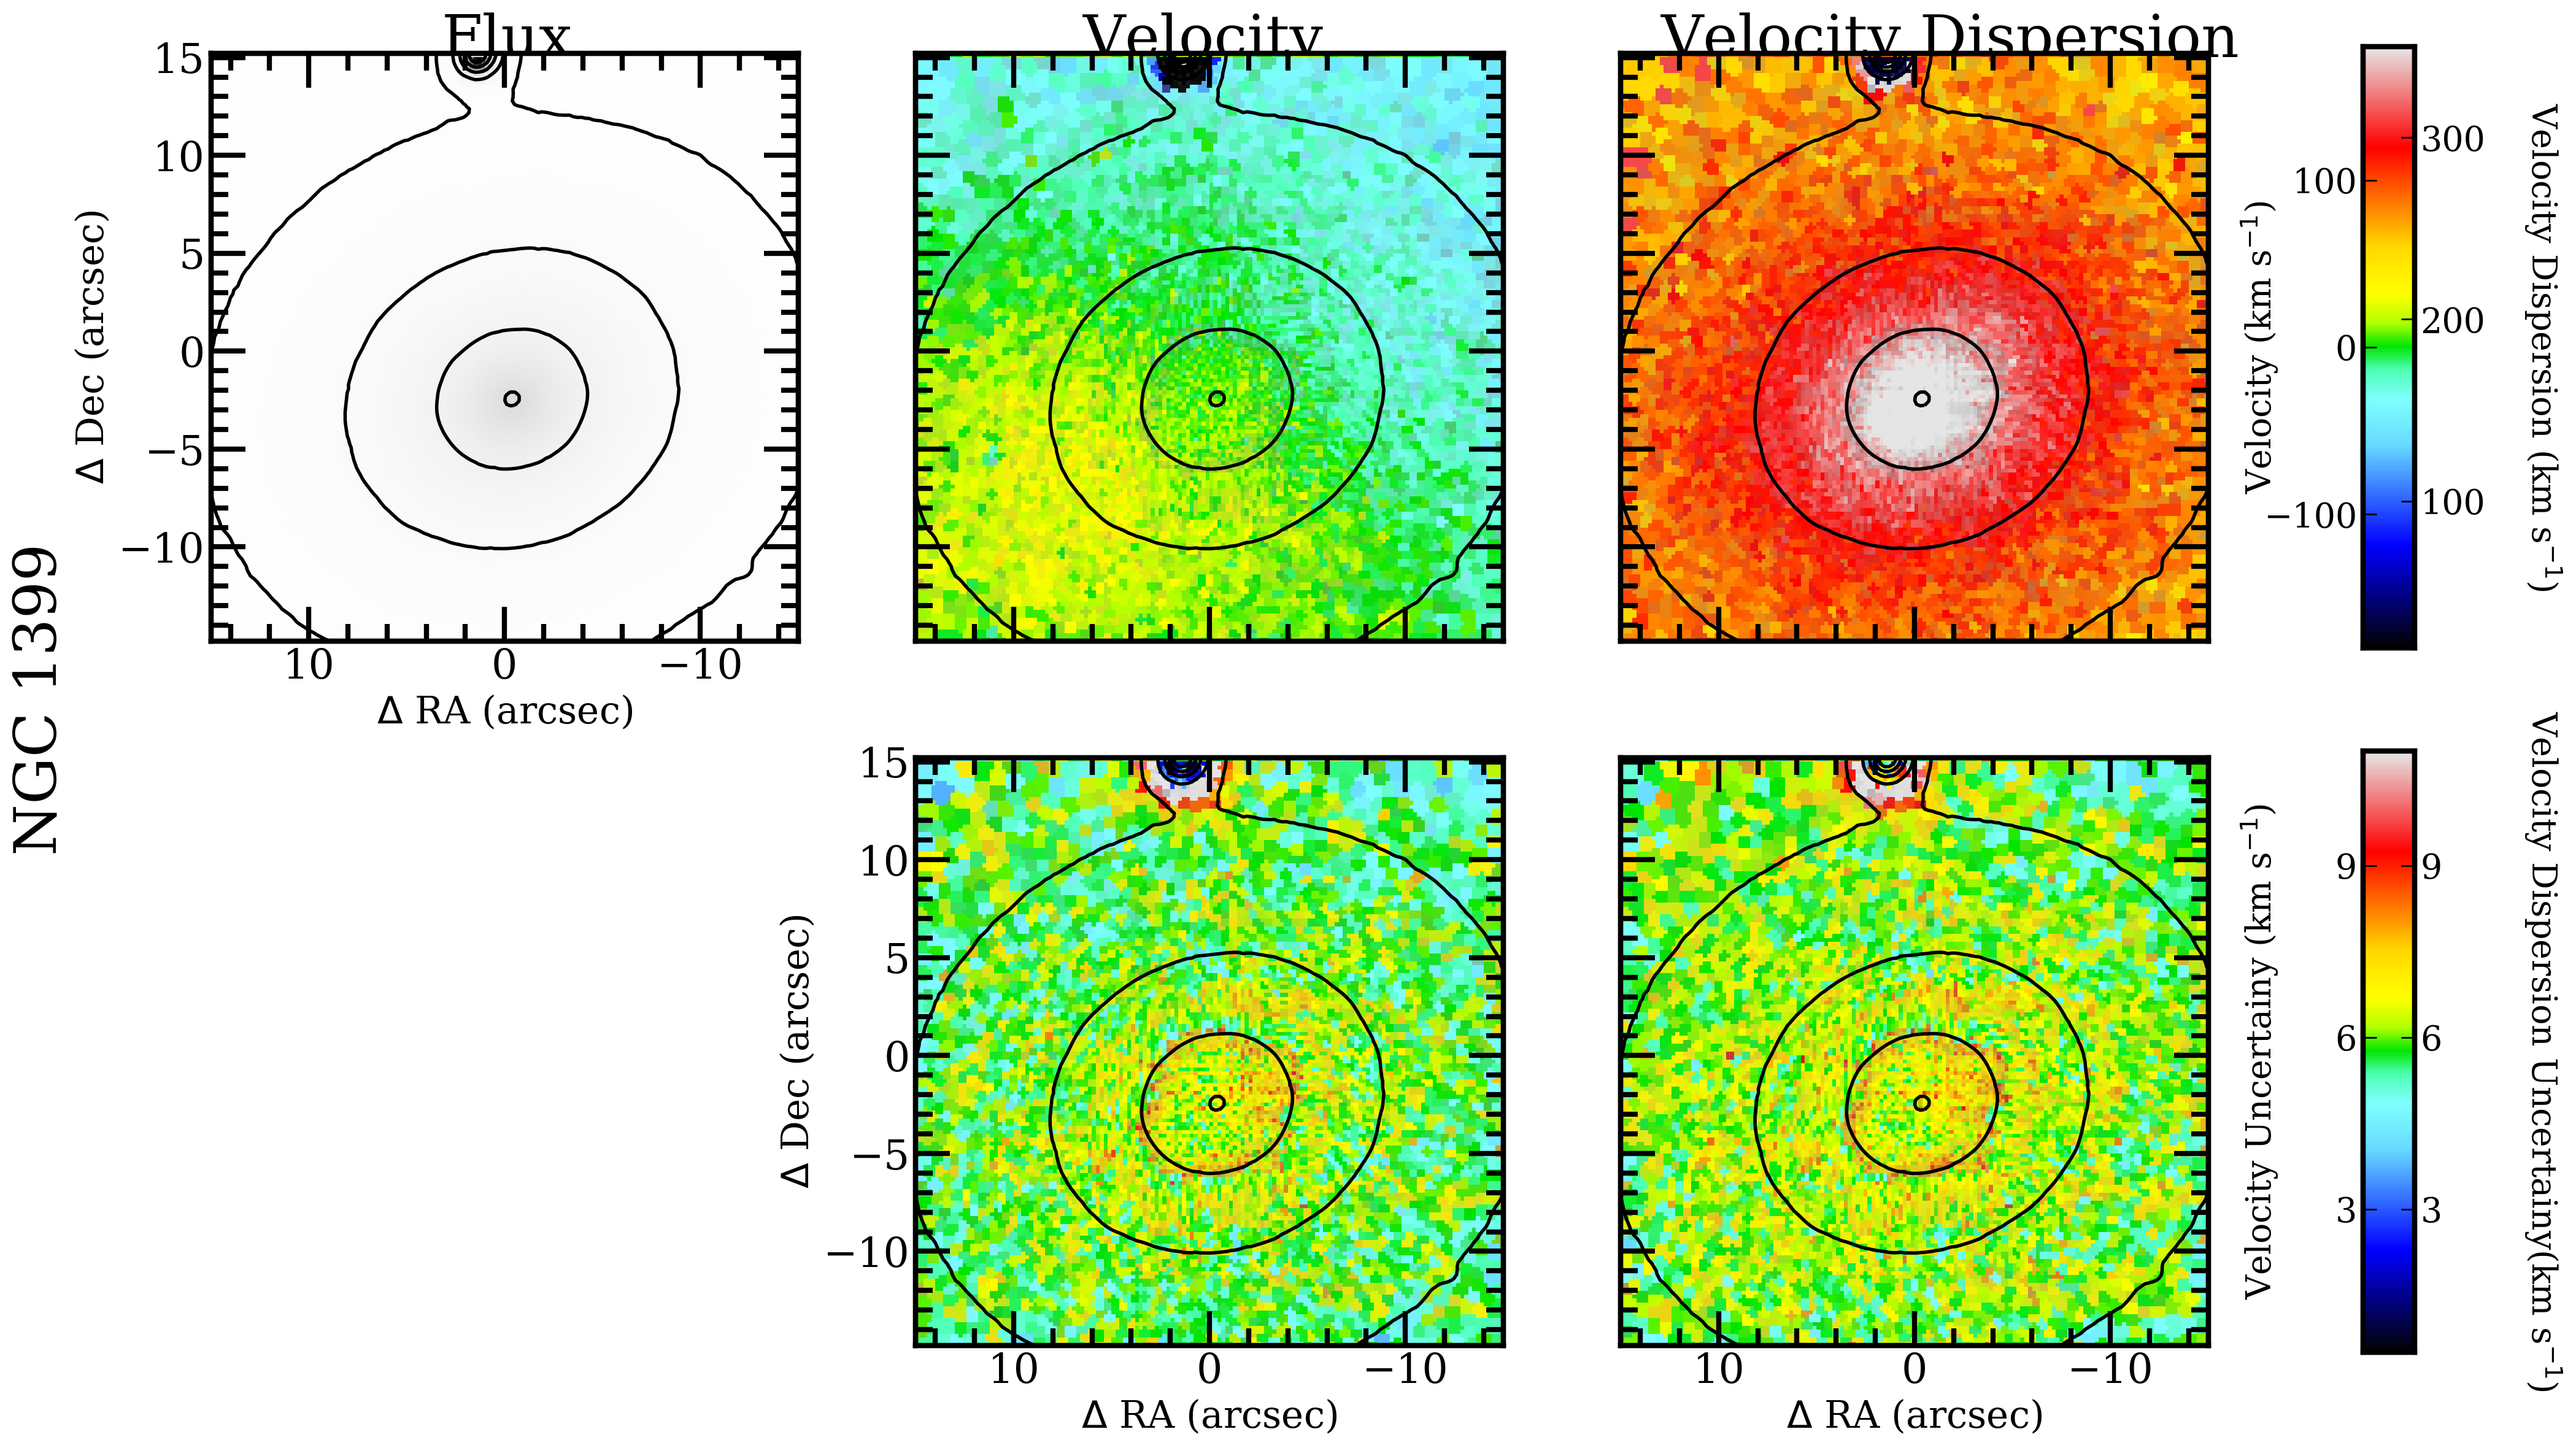
\includegraphics[height=0.31\textheight]{chapter4/muse/kin2.png}
			\contcaption{\textit{Continued.}}
		\end{figure}



		\begin{table}
			\centering
		\begin{threeparttable}
			\caption{Kinematic classifications}
			\label{tab:classify}
			\begin{tabular}{l c c c c c c c}
				\hline
				\hline
				Galaxy		& $\lambda_\mathrm{R_e}$ & $\epsilon_\mathrm{e}$  & $\Gamma_\text{kin}$ (deg) & FR/SR 	& RR/NRR 	& Feature & Group 	\\
				\hline 
				ESO 443-G024 & 0.048 & 0.35 & $-18\pm\leavevmode\phantom{0}2$	& SR & NRR & KDC & c \\
				IC 1459 	& 0.125 & 0.24 & \leavevmode\phantom{0}$-3\pm\leavevmode\phantom{0}1$ & SR & NRR & KDC & c \\
				IC 1531 	& 0.101 & 0.08 & $-54\pm25$	& FR & NRR & LV & a \\
				IC 4296		& 0.034 & 0.03 & \leavevmode\phantom{$-0$}$8\pm12$ & SR &\leavevmode\phantom{N}RR & -- & e \\
				NGC 612 	& 0.655 & 0.36 & \leavevmode\phantom{$-$}$12\pm\leavevmode\phantom{0}6$	& FR &\leavevmode\phantom{N}RR & -- & e \\
				NGC 1316 	& 0.100 & 0.39 & \leavevmode\phantom{$-0$}$6\pm\leavevmode\phantom{0}2$ & FR & NRR & -- & f \\
				NGC 1399 	& 0.090 & 0.12 & $-74\pm\leavevmode\phantom{0}5$ & SR & NRR & LV & a \\
				NGC 3100 	& 0.354 & 0.24 & \leavevmode\phantom{0}$-8\pm\leavevmode\phantom{0}2$ & FR &\leavevmode\phantom{N}RR & -- & e \\
				NGC 3557 	& 0.312 & 0.20 & \leavevmode\phantom{$-$}$16\pm\leavevmode\phantom{0}5$ & FR &\leavevmode\phantom{N}RR & -- & e\\
				NGC 7075 	& 0.068 & 0.04 & \leavevmode\phantom{$-$}$36\pm50$ & SR & NRR & -- & b \\
				PKS 718-34  & 0.159 & 0.17 & \leavevmode\phantom{$-$}$15\pm25$ & FR & NRR & KDC\tnote{a} & b\\
				\hline
				\hline
			\end{tabular}
			\begin{tablenotes}
			\footnotesize
			\note Col.\,1: Galaxy name. Col.\,2: $\lambda_\mathrm{R}$ evaluated at $R_\mathrm{e}$. Col.\,3: Ellipticity at $R_\mathrm{e}$. Col.\,4: Misalignment angle between the kinematic and photometric position angles. Col.\,5: Fast-/slow-rotator (FR/SR) classification. Col.\,6: Regular-rotator (RR) or non-regular-rotator (NRR). Col.\,7: Kinematic features: kinematically-decoupled core (KDC) or low-velocity (LV). Col.\,8: Kinematic group.
			\item [a] Tentative classification. A higher signal-to-noise ratio (S/N) in the outer regions of the field of view is required for confirmation.
			\end{tablenotes}
		\end{threeparttable}
		\end{table}

		The stellar kinematics of the sample galaxies are classified according to the regular rotator/non-regular rotator (RR/NRR) categories of \citet{Krajnovic2011}, with the results listed in Col.\,6 of Table \ref{tab:classify}. Here and hereafter, where MUSE datacubes exist their derived properties are quoted. Otherwise the values are derived from the VIMOS datacubes. We find 4/11 of our sample galaxies are regular rotators. This compares to 82\% of the Atlas$^\text{3D}$ sample being classified as regular rotators \citep{Krajnovic2011}. However the likelihood of a given galaxy being a regular rotator is highly mass dependent with the likelihood decreasing with increasing mass. Thus since our Southern sample are all extremely massive galaxies, we expect to find a higher fraction of non-regular rotators than the Atlas$^\text{3D}$ survey. 

		In addition to this, we attempt to identify the kinematic features defined by \citet{Krajnovic2011} in an algorithmic way. However, the artefacts from the VIMOS quadrants (see Section \ref{subsec:VIMOSartefacts}) confuse ellipse fitting algorithms so only maps derived from the MUSE data are classified in this way; kinematic features in maps derived from the VIMOS data are identified by eye. These classification are listed in Col.\,7 of Table \ref{tab:classify} and the corresponding kinematic group (see Table \ref{tab:KinGroups} and Fig.\,\ref{fig:EgSubstructure} for group definitions and examples) to which a given galaxy belongs to is given is Col.\,8. We observe 3 KDCs (although PKS 718-34 is only a tentative classification) such that $29\pm19$\% of non-regular rotators in our Southern sample definitely (not including PKS 718-34) contain KDCs (or $43\pm19$\% including PKS 718-34), with the large uncertainty reflecting the low-number statistics. This is consistent with the Atlas$^\text{3D}$ survey who found find $25\pm7$\% of non-regular rotators host KDCs \citep{Krajnovic2011}.

		\subsubsection{Robustness of Stellar Results}
			\label{subsubsec:RobustKin}
			Given the problems with the reduction and analysis of VIMOS data, as outlined in Section \ref{VIMOSartefacts}, it is necessary to examine the robustness of these results. Firstly, in Figures \ref{fig:ppxf1} -- \ref{fig:ppxf4}, we show the best-fitting spectra for 3 locations (as marked in the reconstructed images with a number, 1--3) in IC 1459 and IC 4296 for both VIMOS and MUSE datacubes. 

			%Whilst, on first inspection, it may seem that both VIMOS and MUSE have similar quality data in terms of cleanliness, it is worth noting that each spaxel in VIMOS has $>11$ times the collecting area of each spaxel in MUSE, and that the exposure time for the VIMOS data was $>16$ that of the corresponding MUSE data.

			As can be seen from the small values of and lack of obvious sign of correlation within the residuals (green dots) the best-fitting total spectra (red line) are good fits to the data (black line). The best-fitting emission lines are shown in yellow. Given the coincidental alignment in these figures of H$\beta$ and [\ion{O}{iii}] in the VIMOS spectra with [\ion{N}{ii}], H$\alpha$ and [\ion{S}{ii}] in the MUSE spectra, it is worth explicitly pointing out the different wavelength ranges between the MUSE and VIMOS datasets. 

			We can also see some of the bad pixels in the MUSE spectra. These are residuals of the poor sky subtraction by the ESO routines as discussed in Section \ref{subsec:MUSEreduction}. It can also be seen that they do not obviously effect the result of the stellar fit. Since [\ion{O}{iii}] is first fitted, with the kinematics of all other lines tied to that of [\ion{O}{iii}] and that the region surrounding the [\ion{O}{iii}] doublet is free of such residuals, it is likely that the best-fitting [\ion{N}{ii}], H$\alpha$ and [\ion{S}{ii}] lines/doublets are also reliable, despite occurring in regions effected by these residuals. 

			\begin{figure}
				\centering
				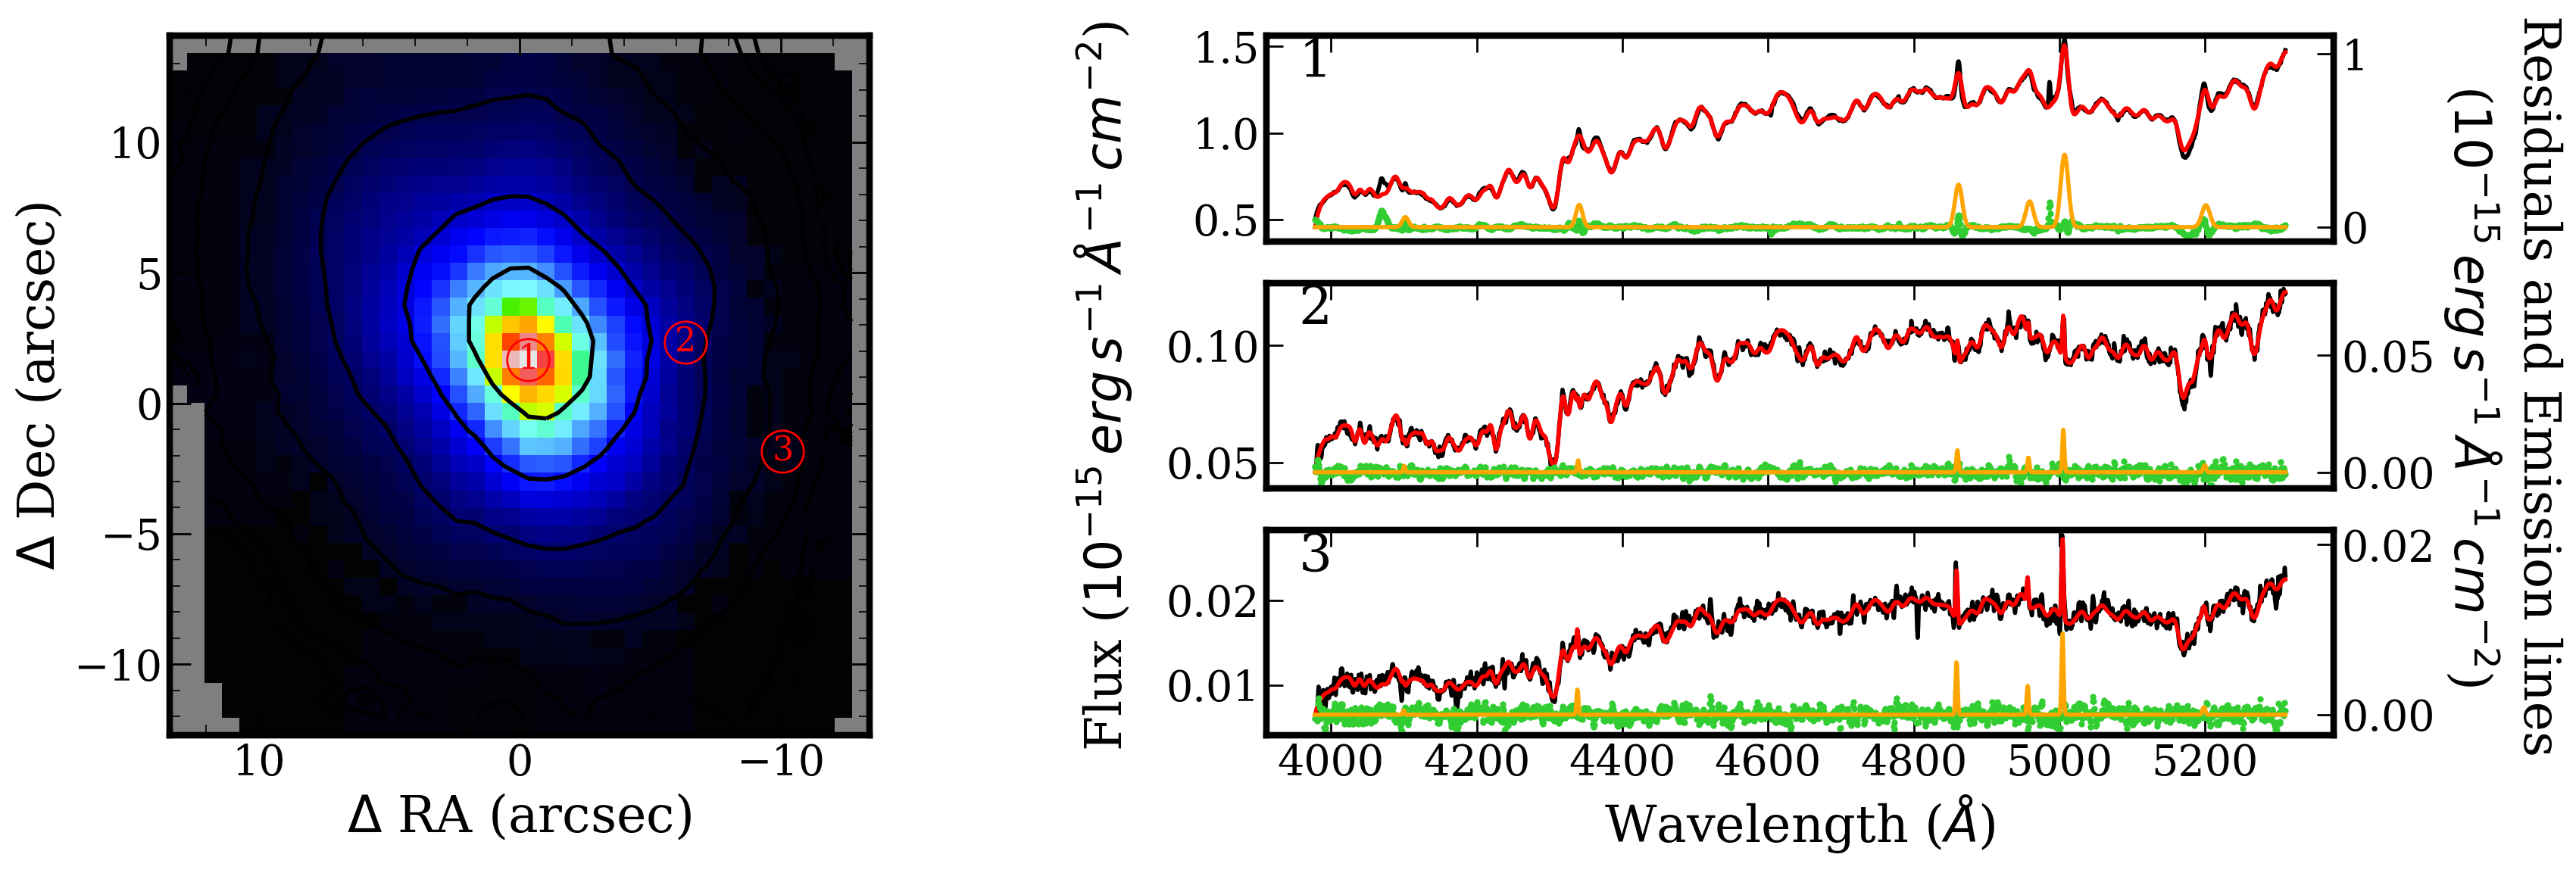
\includegraphics[width=.9\textwidth]{chapter4/pPXF_fits_vimos_ic1459.png}
				\caption[Best-fitting spectra by \textsc{pPXF} for the VIMOS datacube for IC 1459]{The best-fitting spectra (red line) from the \textsc{pPXF} fits to spatially-binned VIMOS spectra (black line) of IC 1459 at 3 locations as corresponding to the locations marked by the red numbering (1--3) in the reconstructed image (right). Residuals (data - best-fitting spectra) and best-fitting emission lines are shown as green dots and orange lines, respectively.}
				\label{fig:ppxf1}
			\end{figure}
			\begin{figure}
				\centering
				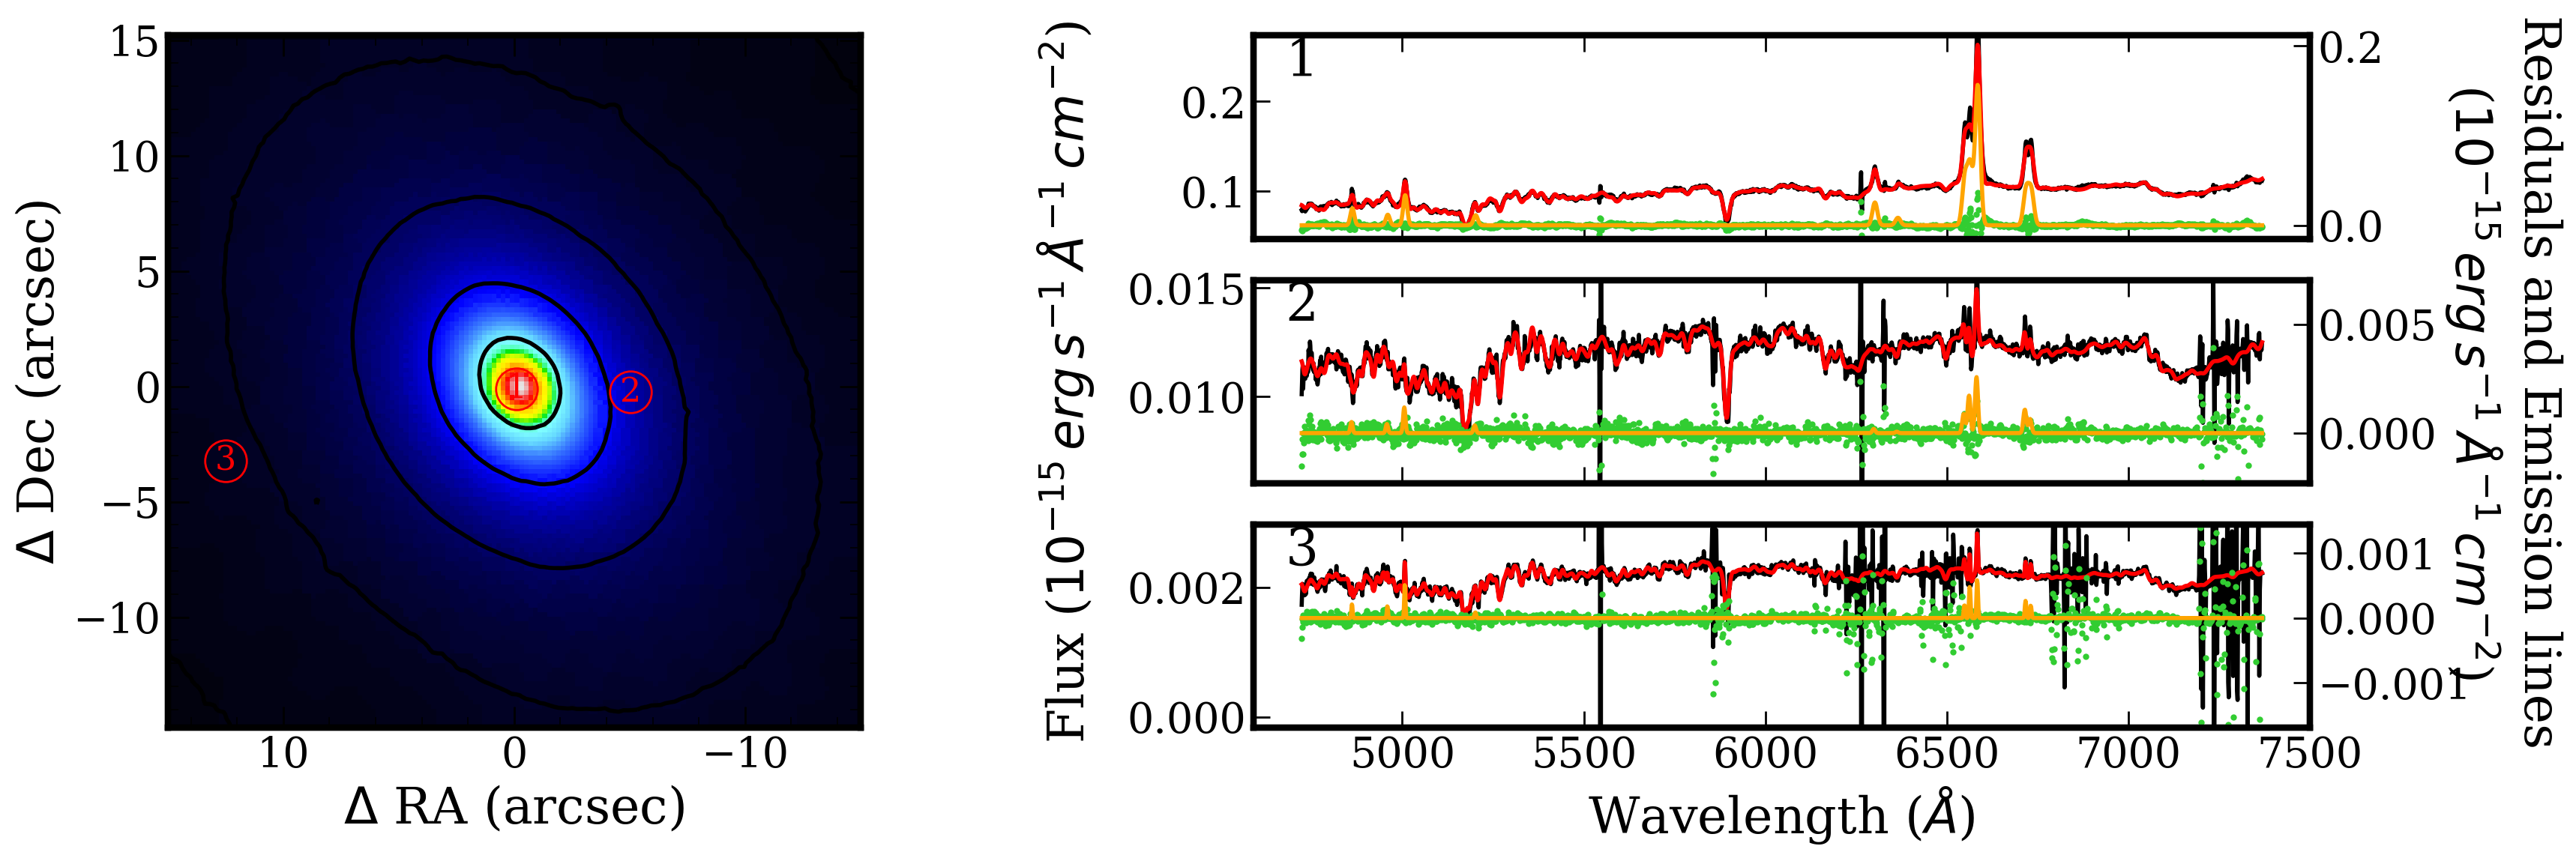
\includegraphics[width=.9\textwidth]{chapter4/pPXF_fits_muse_ic1459.png}
				\caption[Best-fitting spectra by \textsc{pPXF} for the MUSE datacube for IC 1459]{As in Figure \ref{fig:ppxf1} but for MUSE spectra.}
				\label{fig:ppxf2}
			\end{figure}
			\begin{figure}
				\centering
				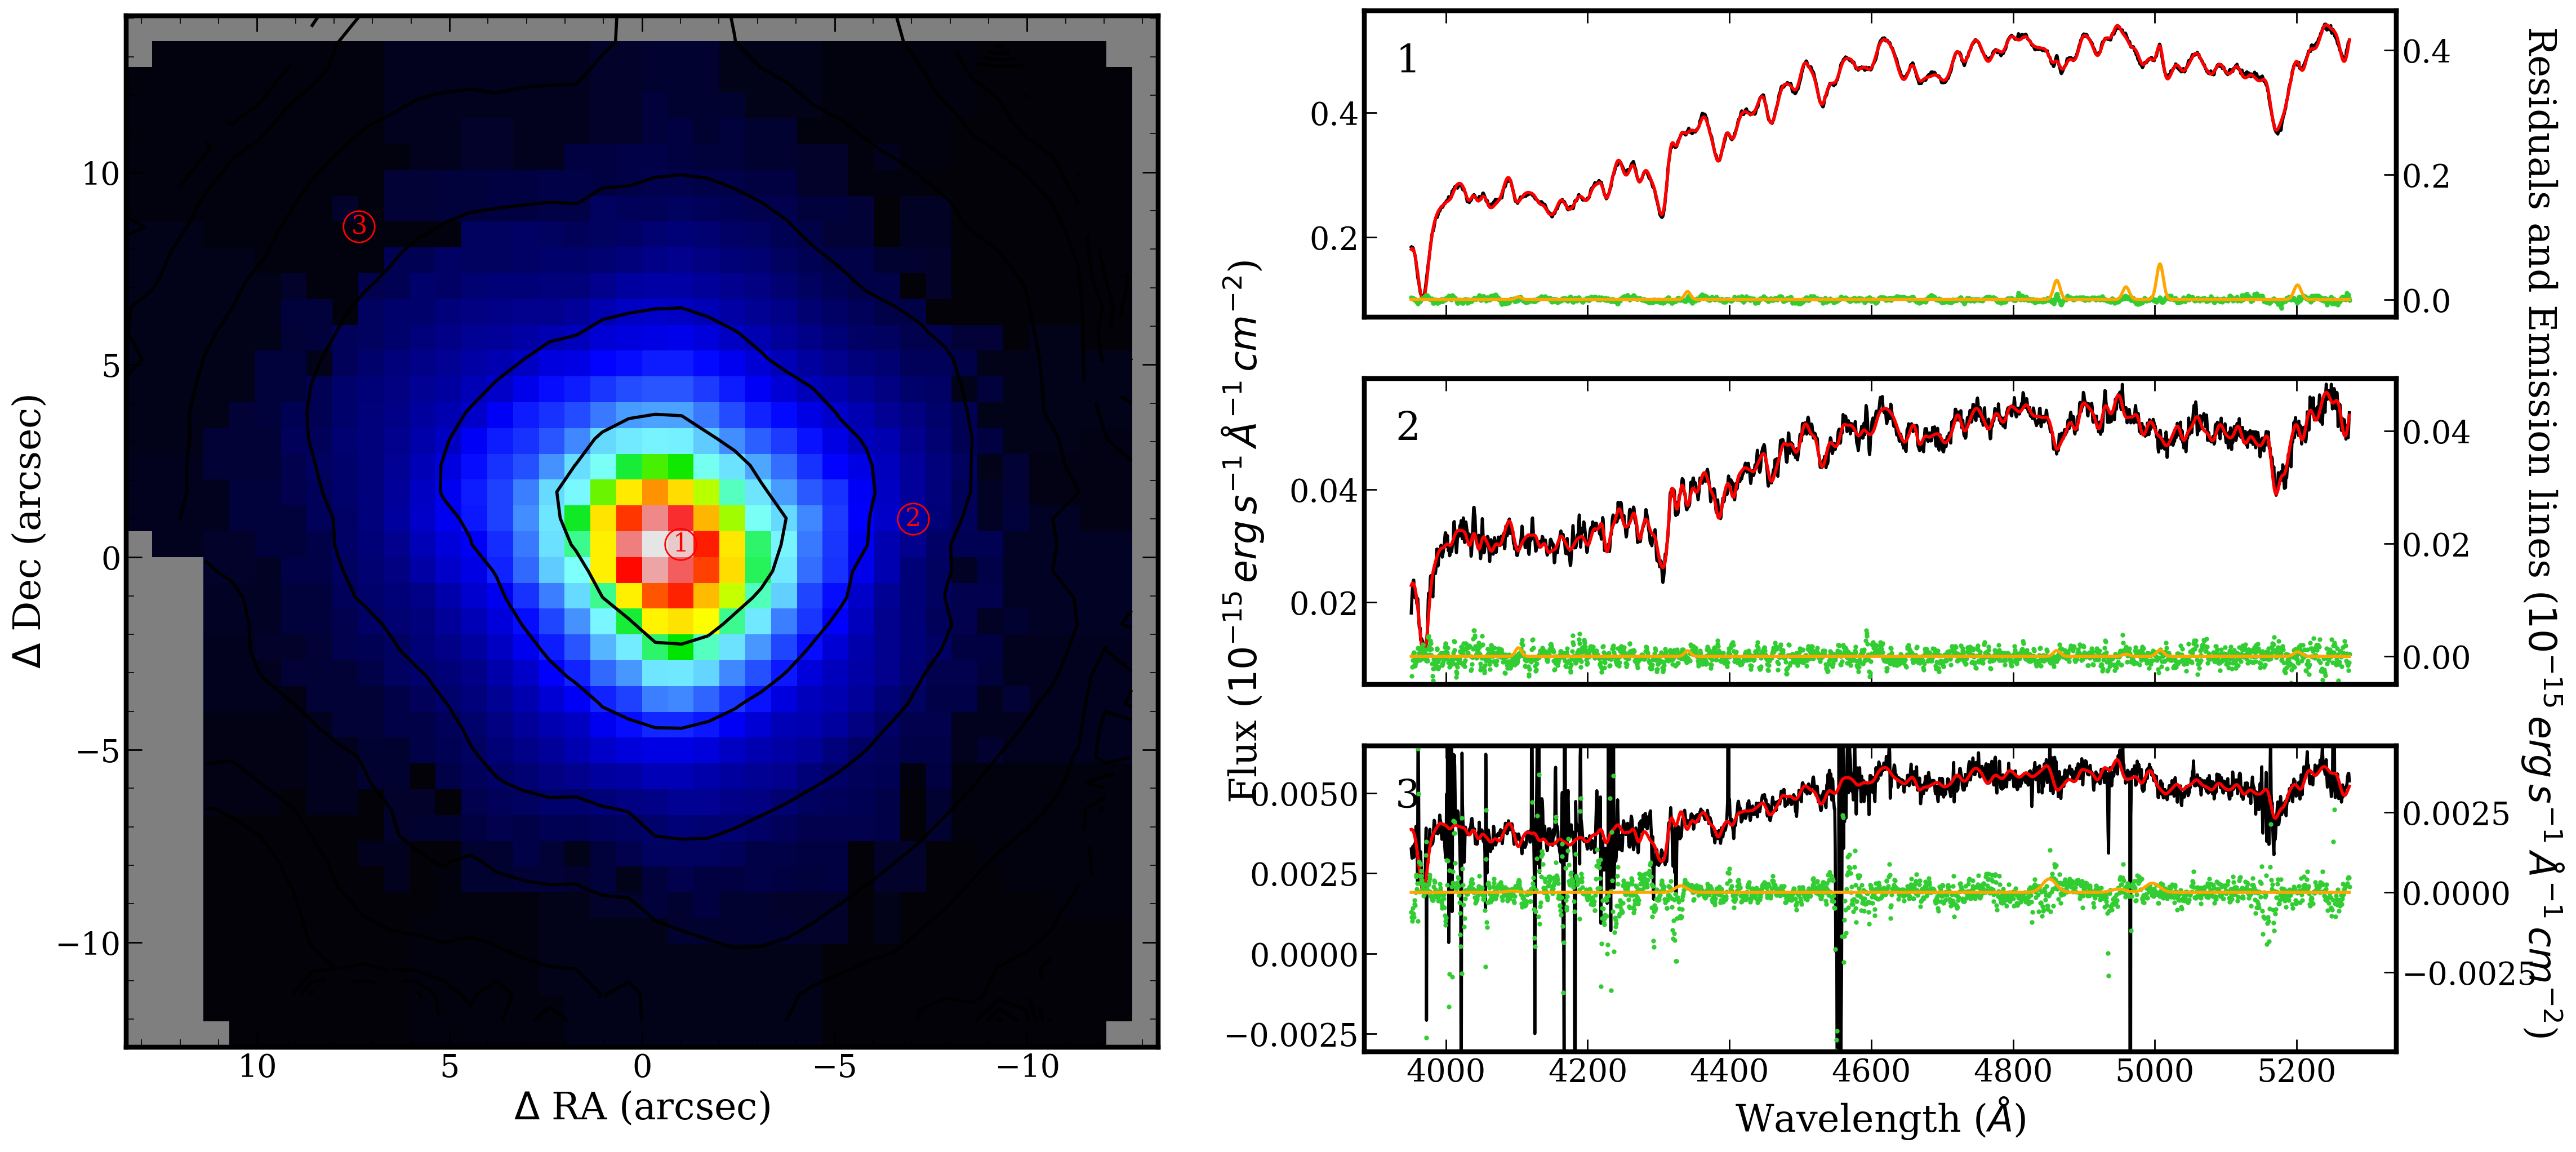
\includegraphics[width=.9\textwidth]{chapter4/pPXF_fits_vimos_ic4296.png}
				\caption[Best-fitting spectra by \textsc{pPXF} for the VIMOS datacube for IC 4296]{As in Figure \ref{fig:ppxf1} but for IC 4296.}
				\label{fig:ppxf3}
			\end{figure}
			\begin{figure}
				\centering
				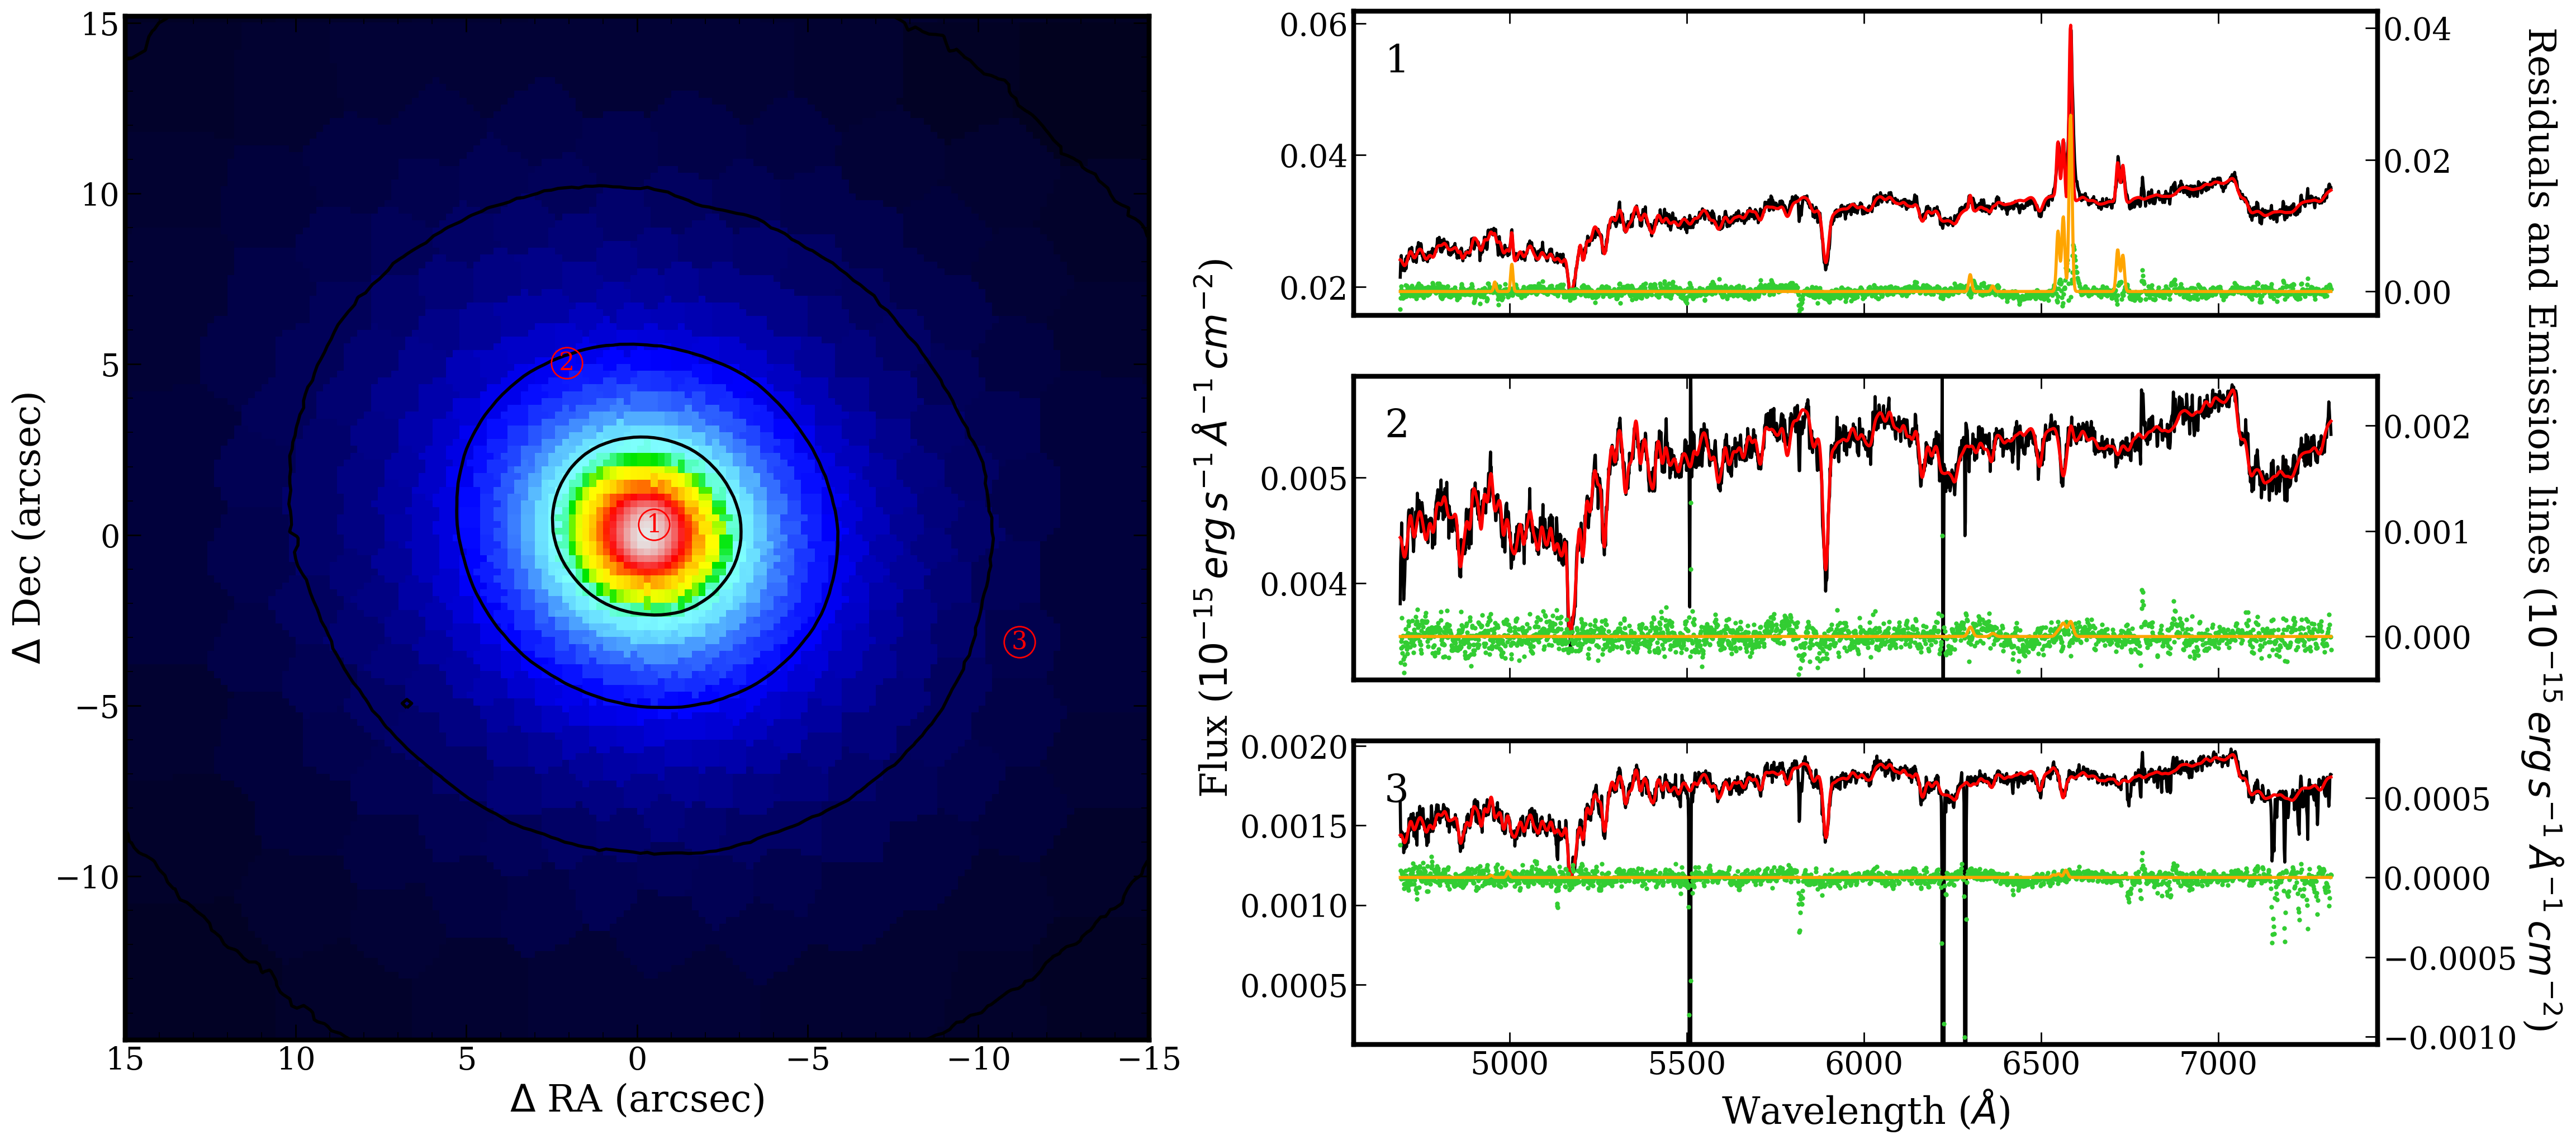
\includegraphics[width=.9\textwidth]{chapter4/pPXF_fits_muse_ic4296.png}
				\caption[Best-fitting spectra by \textsc{pPXF} for the MUSE datacube for IC 4296]{As in Figure \ref{fig:ppxf1} but for MUSE spectra of IC 4296.}}
				\label{fig:ppxf4}
			\end{figure}

			We also directly compare the stellar velocity maps from VIMOS and MUSE (see Fig.\,\ref{fig:compare_velfield}). In IC 4296 and NGC 1399, we see the artifacts from the VIMOS instrument almost entirely obstruct any meaningful interpretation the velocity maps generated from VIMOS data. However in IC 1459, we can see that both instruments give similar results, although some artifact can been seen in the MUSE data (such as the an arrowhead shape above the KDC). 

			\begin{figure}
				\centering
				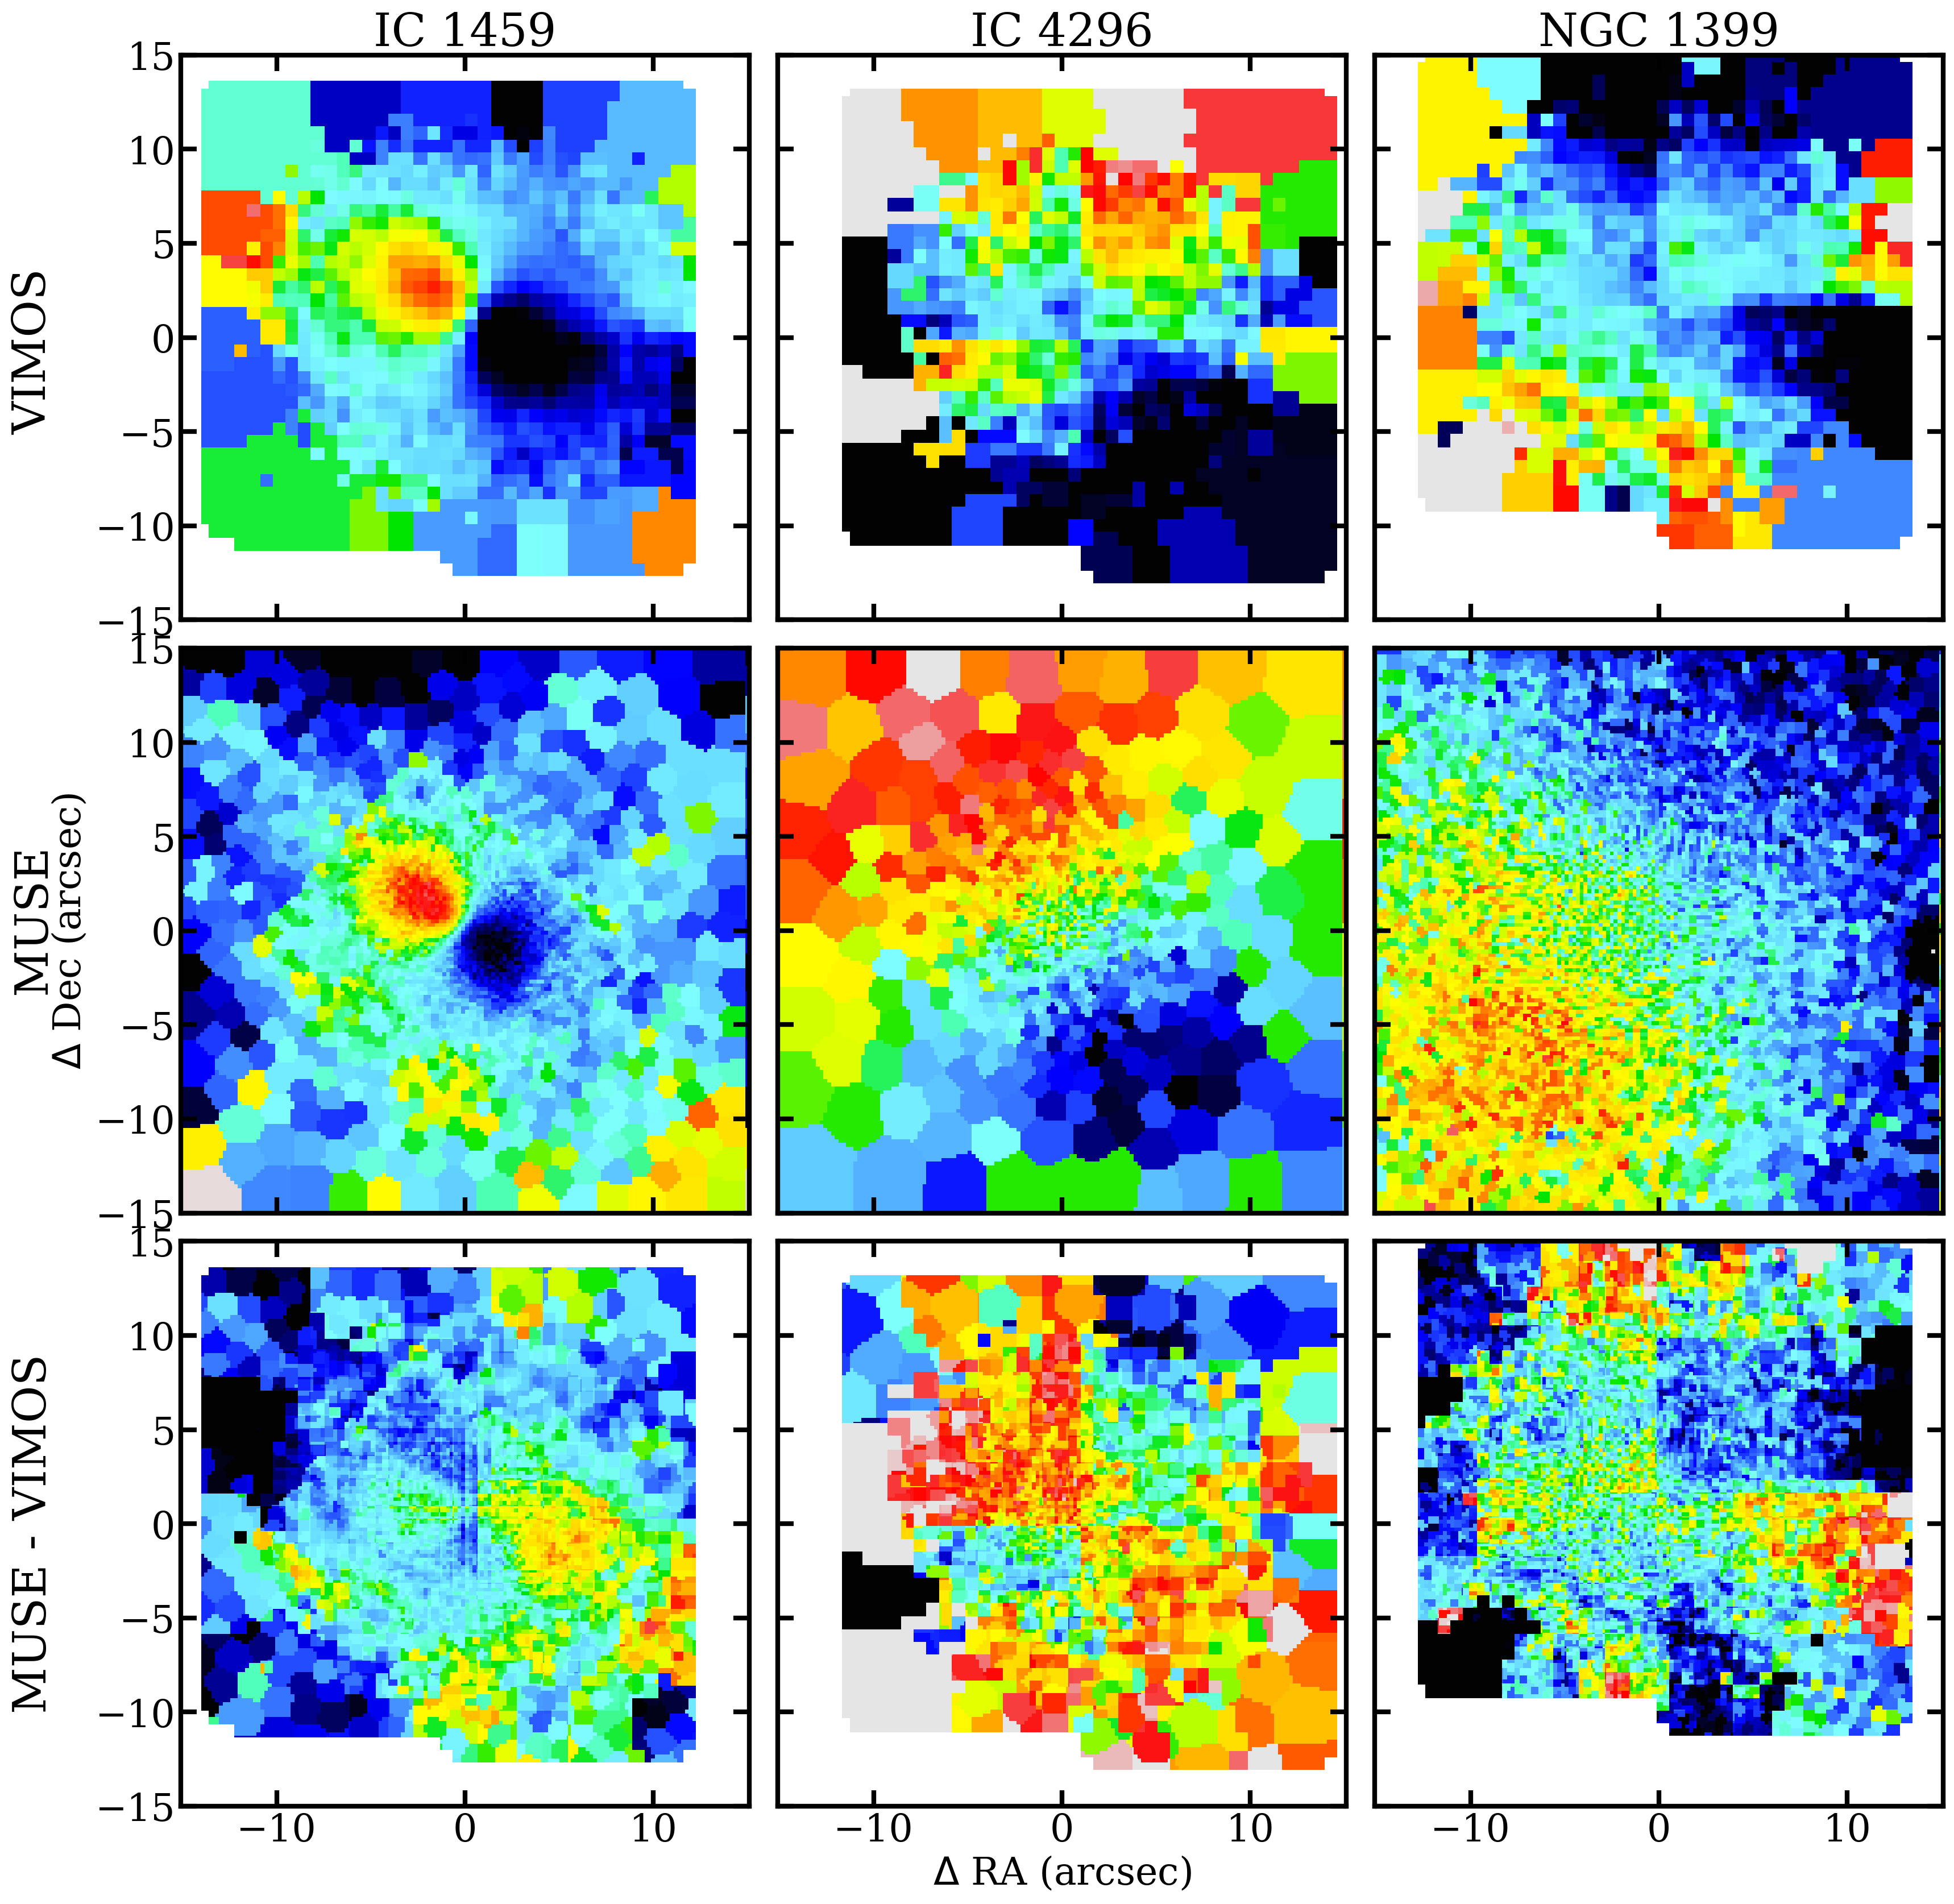
\includegraphics[width=.9\textwidth]{chapter4/compare_velfield.png}
				\caption[Comparison between stellar velocity maps from VIMOS and MUSE datacubes]{A comparison between stellar velocity maps from VIMOS and MUSE datacubes. The top row shows the VIMOS derived maps; the middle row, MUSE derived maps and the bottom row, the residuals of the VIMOS map subtracted from the MUSE map.}
				\label{fig:compare_velfield}
			\end{figure}

			Finally, we compare the radial profiles of the stellar velocity dispersion (see Fig.\,\ref{fig:compare_sigprofile}). Here, we see that in the cases of both IC 1459 and IC 4296 the stellar velocity dispersions are systematically lower for VIMOS data than MUSE. This is particularly noticeable within the inner 5\arcsec. %This may be due to the fact that VIMOS spaxels are over 11 times larger in area than the MUSE spaxels -- but should it not be the other way round? As we are using bin centroid...
			We can also see the degeneration of the VIMOS derived values in IC 1459 at large radii. 
			There are two groups of bins with large ($\approx$600--700\,km\,s$^{-1}$) and small ($\approx 0$\,km\,s$^{-1}$) stellar velocity dispersions at radius $r \approx 17\arcsec$ in NGC 1399 which are outside of the limits of the y-axis which are due to a foreground star to the north of the centre of the galaxy. We excluded this from the plot in order to better show detail of the galaxy's radial stellar velocity dispersion profile.
% needs further comment - have emailed Martin


			\begin{figure}
				\centering
				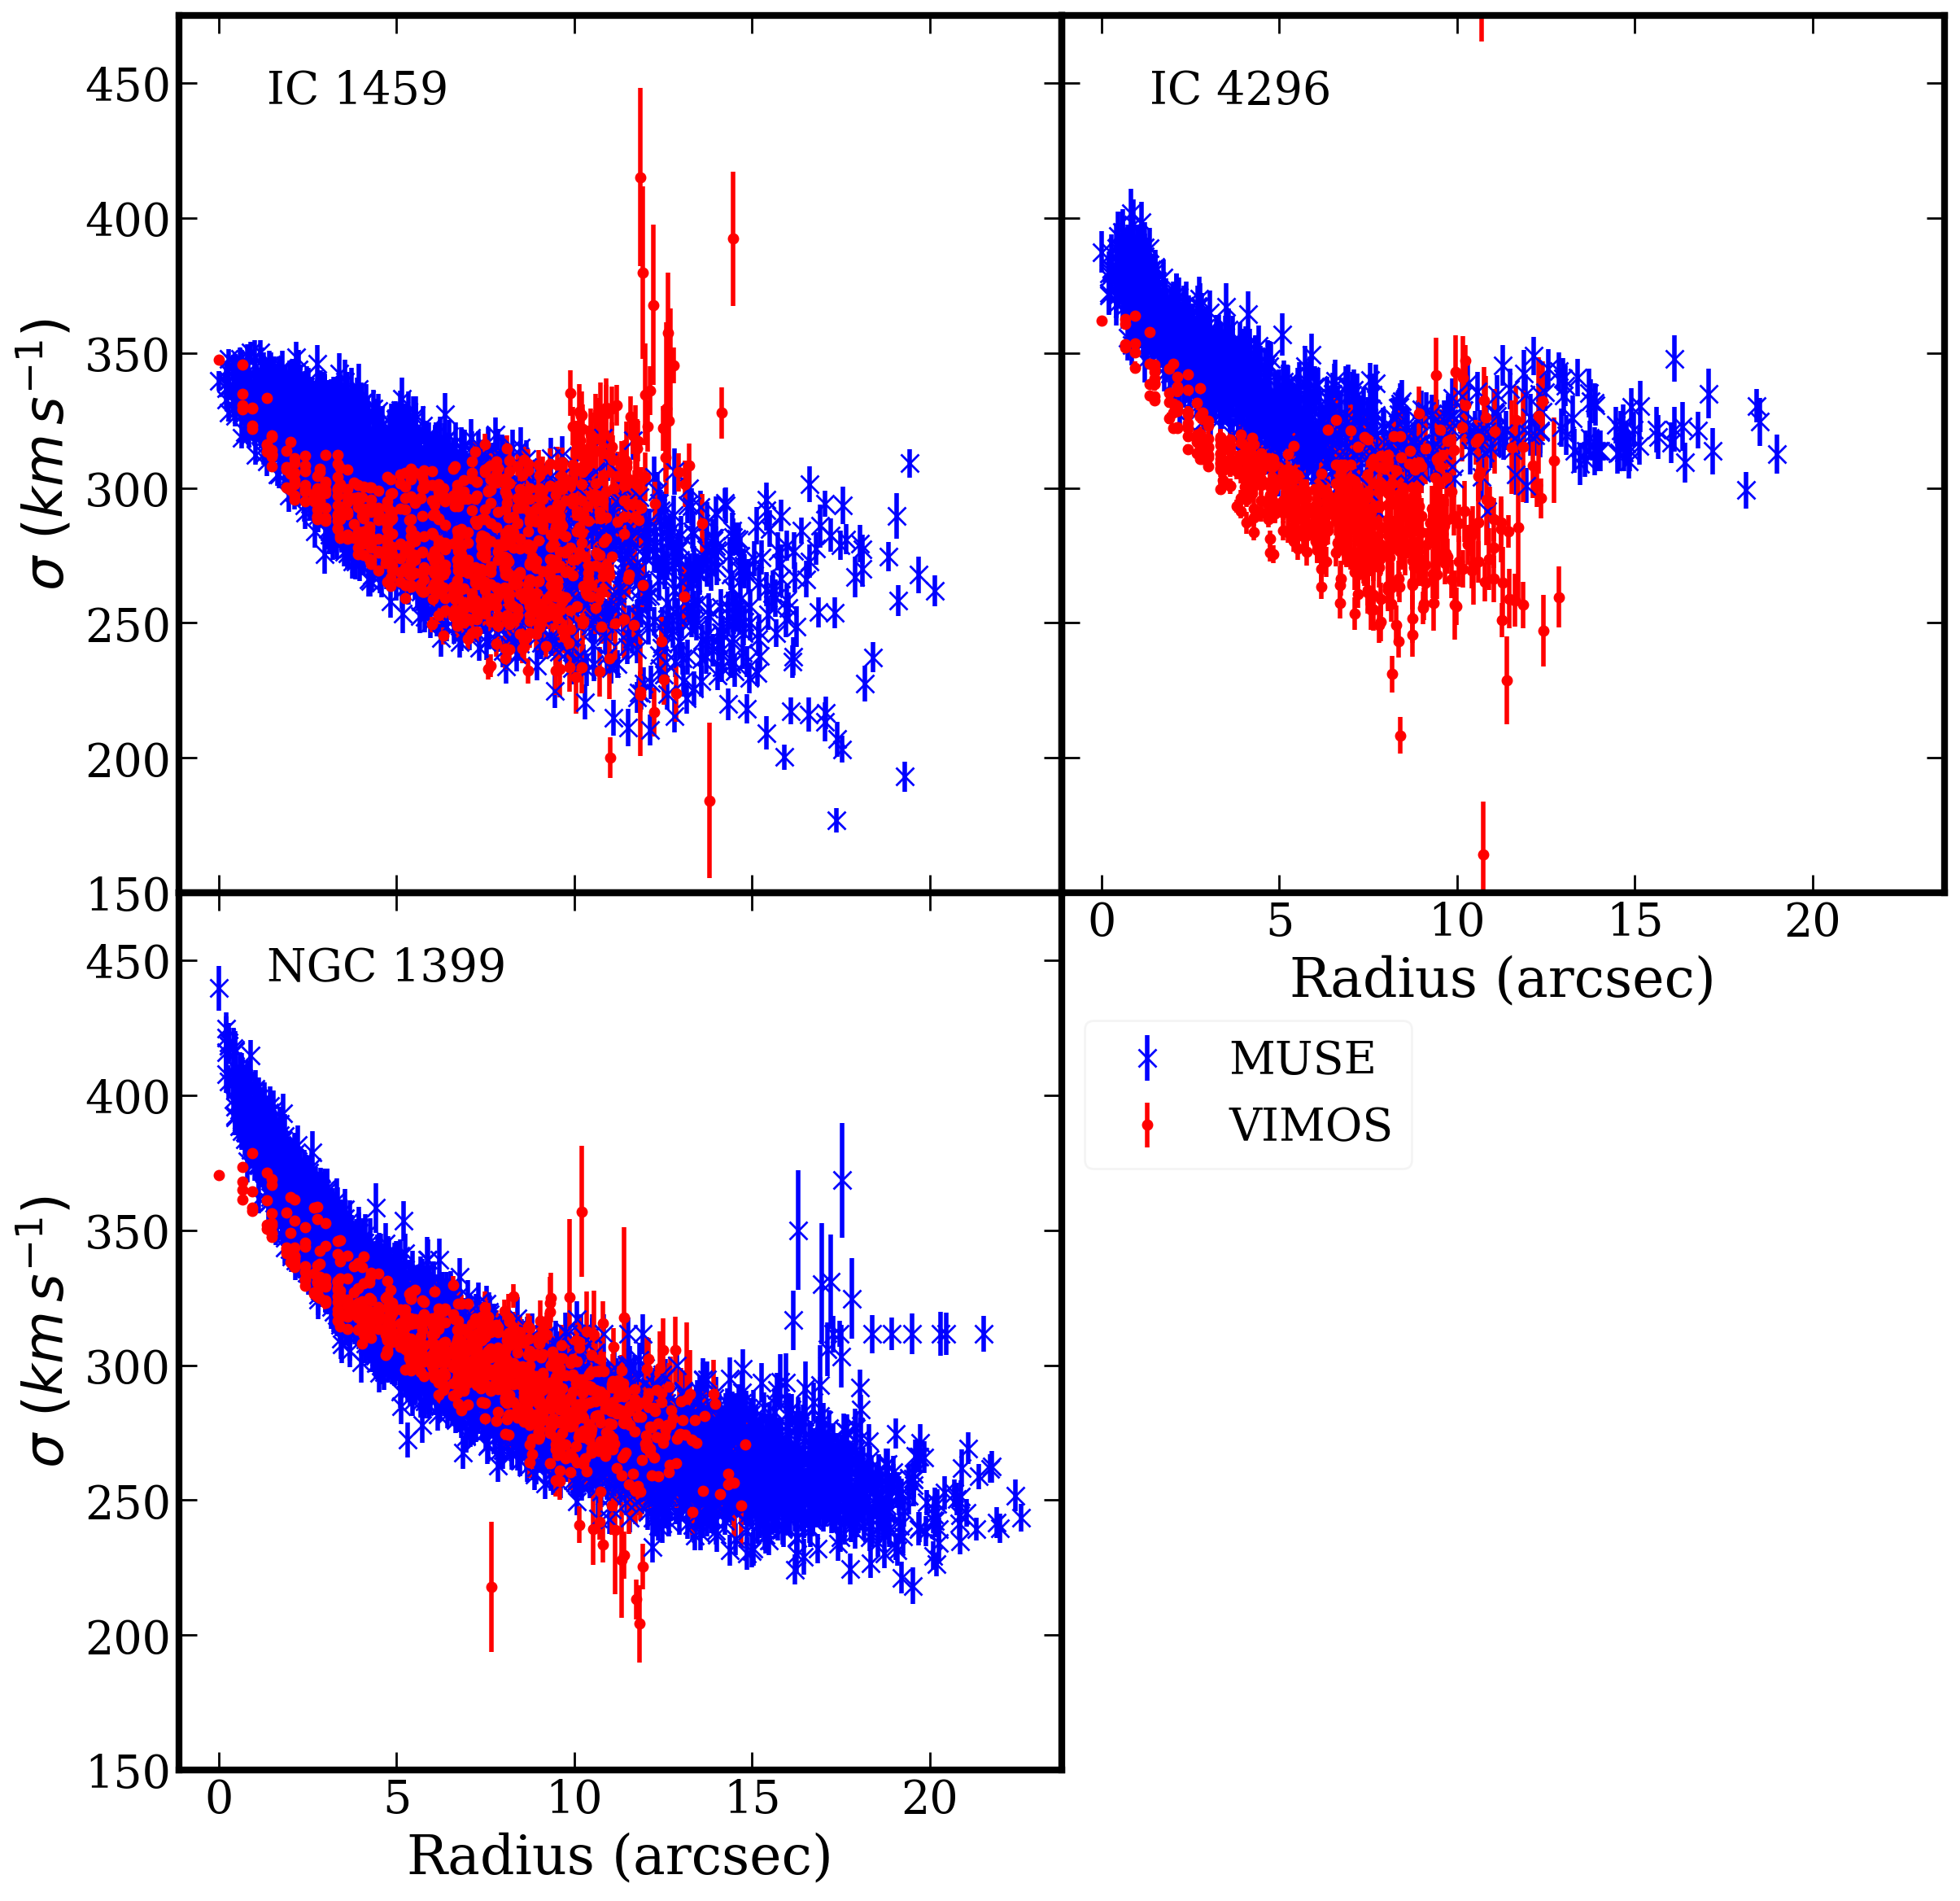
\includegraphics[width=.9\textwidth]{chapter4/compare_sigma.png}
				\caption[Comparison between stellar velocity dispersion radial profiles from VIMOS and MUSE datacubes]{A comparison of the stellar velocity dispersion ($\sigma$) for the VIMOS (red) and MUSE (blue) datasets.}
				\label{fig:compare_sigprofile}
			\end{figure}

			All of the above comparisons show that in the case of IC 1459, which we take as representative of all the well reduced VIMOS datacubes, the best-fitting parameters are consistent with the values of parameters derived from the MUSE datacubes. However IC 4296 and NGC 1399 have (from simple inspection) the strongest artifacts from VIMOS and hence have the worst reduction and least reliability. In fact, as can be clearly seen from some of the Fig.\,\ref{fig:compare_velfield}, the artifacts dominate the spatially resolved maps completely obscuring any structure, however the VIMOS derived parameters still well represent the radial stellar velocity dispersion profile (see Fig.\,\ref{fig:compare_sigprofile}). Similar analysis, with similar conclusions, but for measured absorption line strengths and best-fitting emission lines, is shown in Sections \ref{subsec:RobustAbs} and \ref{subsec:RobustEmi}, respectively.


	\subsection{Ellipticity}
		\label{subsec:Ellipticity}

		\begin{figure}
			\centering
			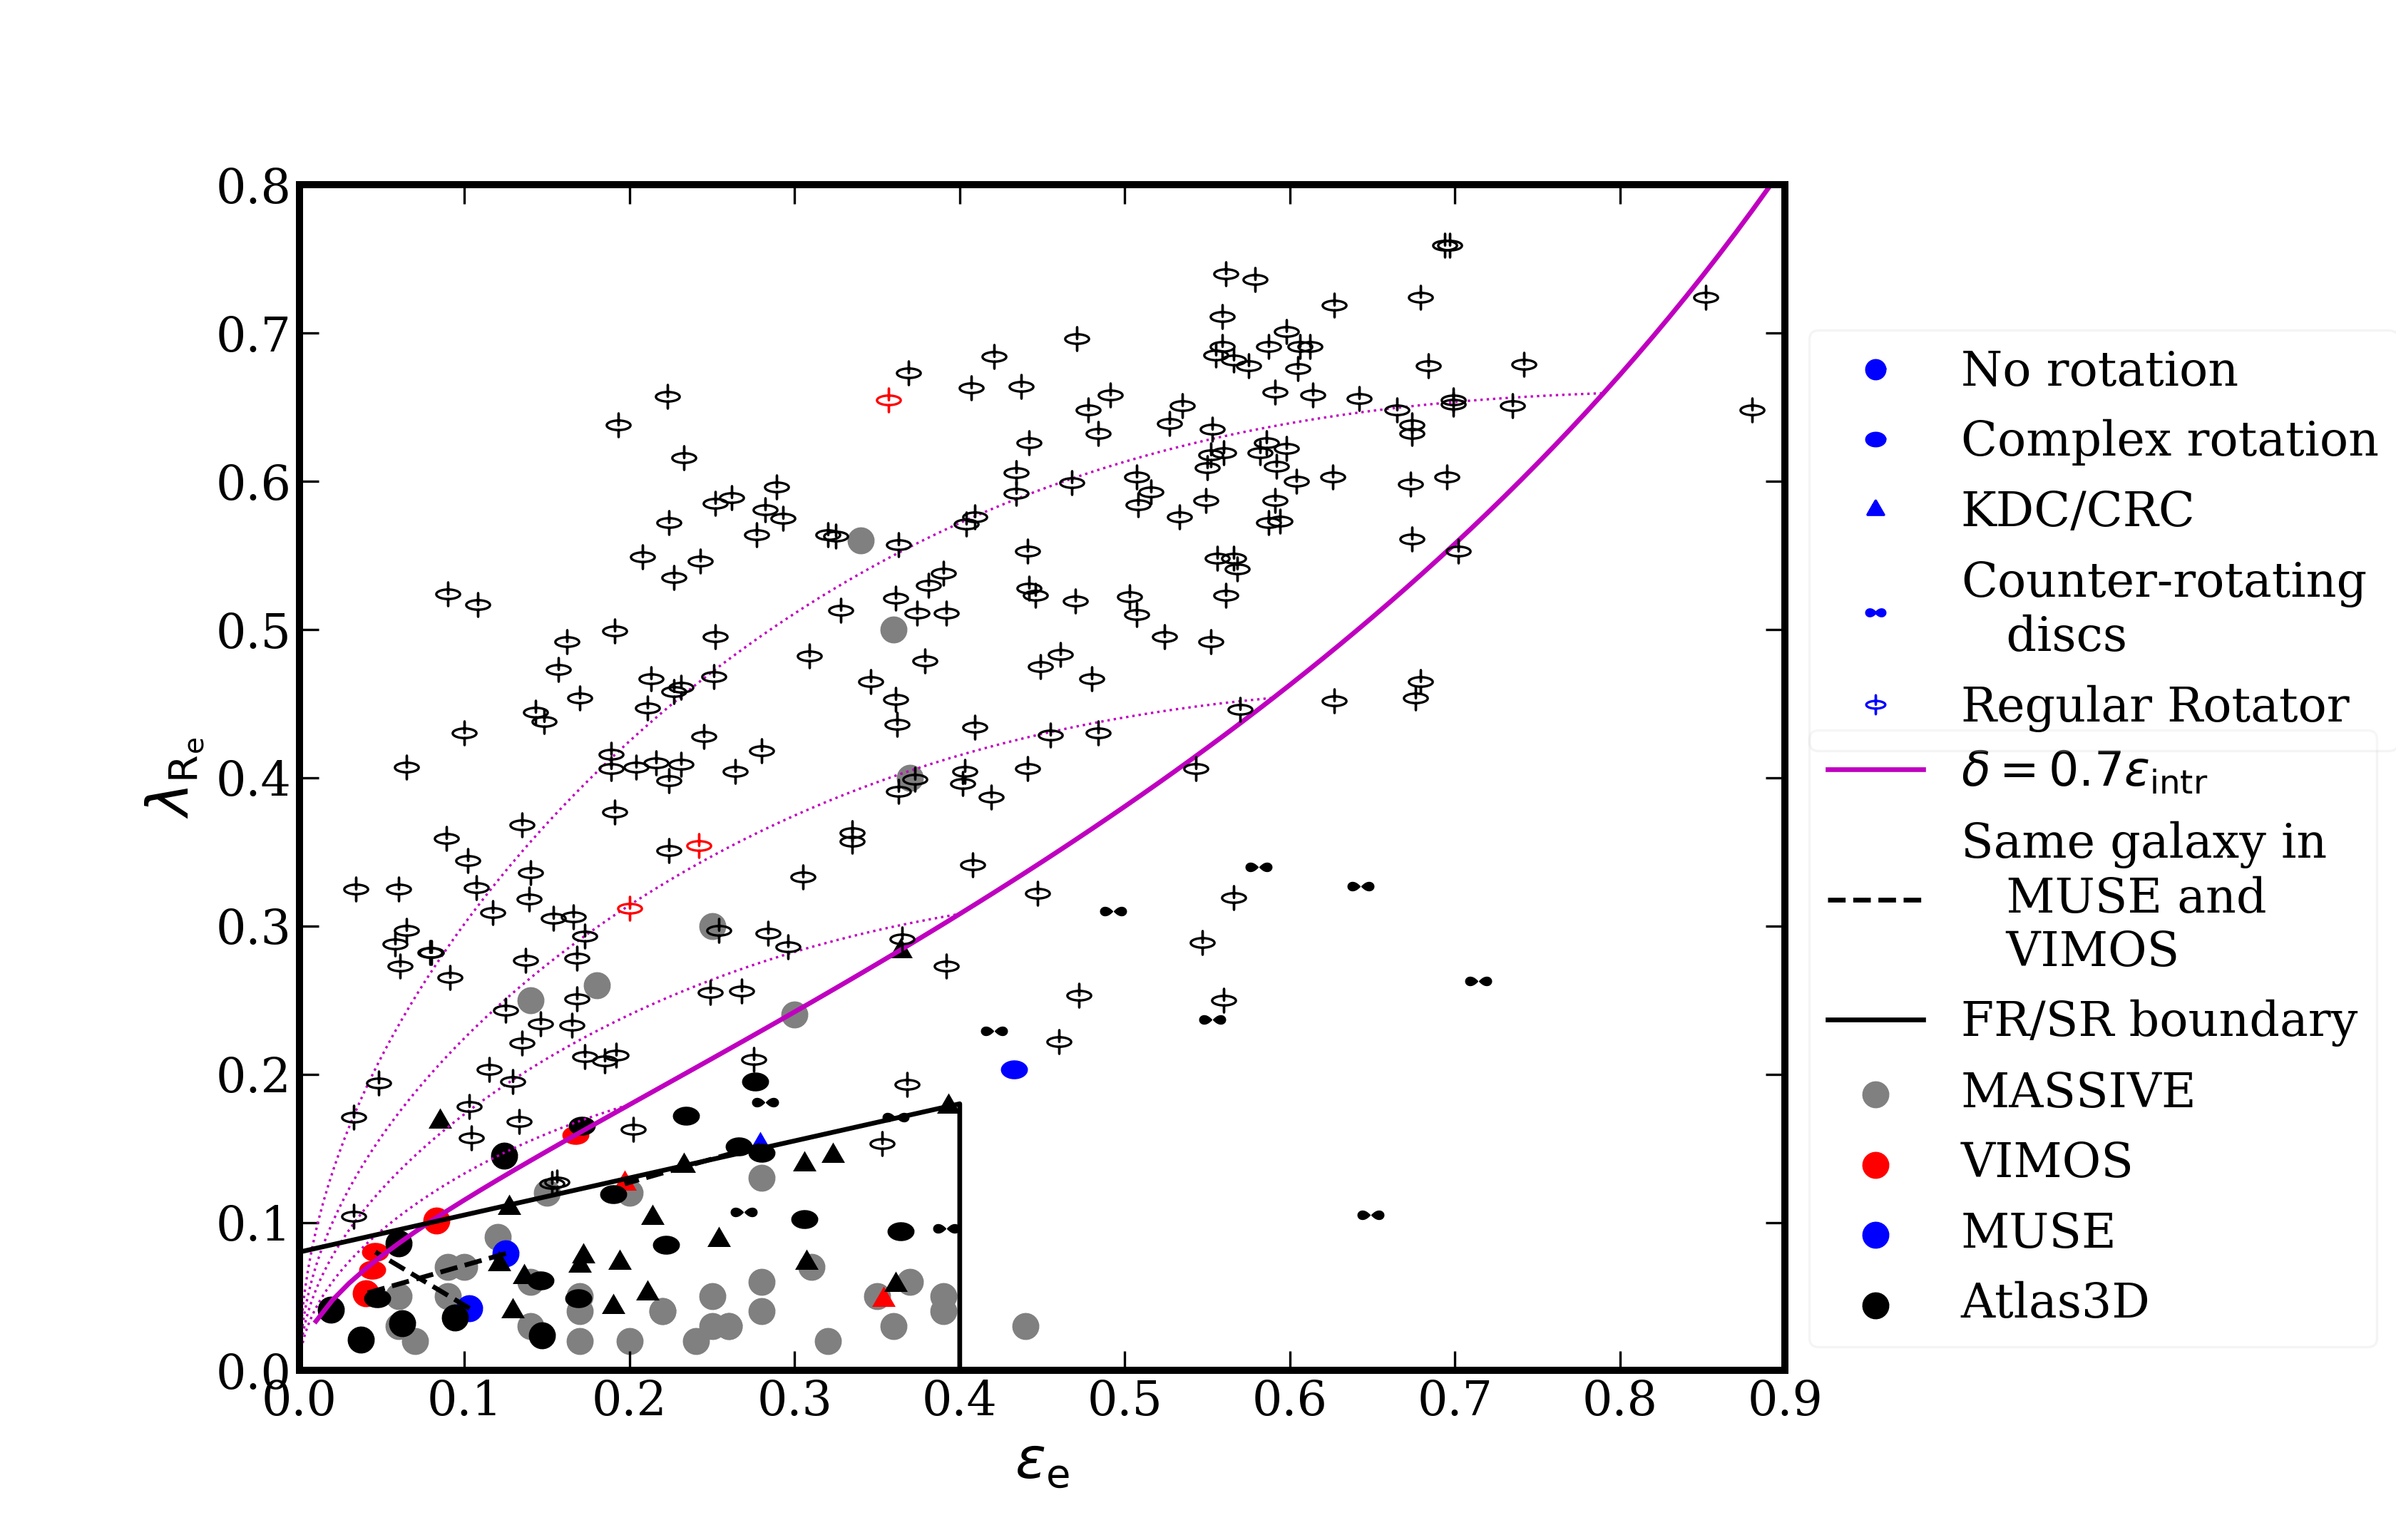
\includegraphics[width=.9\textwidth]{chapter4/lambda_R_ellipticity.png}
			\caption[$\lambda_\mathrm{R_e}$\,--\,ellipticity diagram]{$\lambda_\mathrm{R_e}$\,--\,ellipticity diagram. VIMOS and MUSE measurements are shown in red and blue, respectively. For comparison, Atlas$^\text{3D}$ galaxies \citep{Emsellem2011} are shown in black and MASSIVE galaxies \citep{Veale2017} in grey. The theoretical limit (edge-on systems) of disc-dominated galaxies is shown in solid magenta, with lines of constant intrinsic angular momentum but varying inclination in dotted magenta. The black solid lines show the limits of the fast-/slow-rotator classes. The MASSIVE survey does not report substructure, so the MASSIVE sample galaxies are shown with filled circles.}
			\label{fig:lambdaR_ellip}
		\end{figure}

		Ellipticity is measured as the ellipticity of the best-fitting ellipse to the surface-brightness map with an mean radius $R_\mathrm{m}$, of 1 effective radius $R_\mathrm{e}$. Firstly the centre of the galaxy is found as the luminosity weighted centre using the \textsc{python} routine \textsc{find\_galaxy}, which is part of the \textsc{mge} package\footnote{\url{http://www-astro.physics.ox.ac.uk/\~mxc/software/}} by \citet{Cappellari2002}. This is then used as an input for the \textsc{idl} routine \textsc{kinemetry}\footnote{\url{http://davor.krajnovic.org/idl/}} by \citet{Krajnovic2006} which finds the best-fitting ellipses at a range of evenly spaced semi-major axes. This is achieved by performing harmonic expansion of maps along ellipses with a given semi-major axis and, when used for even moments (e.g.\ surface brightness, velocity dispersion, h$_4$ etc.), minimizing the amplitude of the first and second harmonics. The results include the ellipticity, $\epsilon$ and position angle $PA_\text{phot}$ of the best-fitting ellipse for each semi-major axis. The fit is repeated for increasing semi-major axis until $<$75\% of the ellipse is not contained within the field of view.

		In reality, the field of view does not always contain 1 $R_\mathrm{e}$. Where this is the case, we follow the method by \citet{Emsellem2007}, where $R_\mathrm{m}$ is redefined as $R_\mathrm{m} \equiv \sqrt{A_\mathrm{s}/\pi}$, where $A_\mathrm{s}$ is the area of the ellipse contained within the field of view. For a given galaxy, we fit ellipses as described above, up to $R_\mathrm{m} = R_\mathrm{max}$, where $A_\mathrm{s}$ reaches a maximum difference of 15\% to the area of the fitted ellipse, $A_\text{ellipse}$. The value $\epsilon_\mathrm{e}$, the ellipticity at 1 $R_\mathrm{e}$ or $R_\text{max}$, whichever is smallest, is given in Table \ref{tab:classify}. 

	\subsection{Fast-/Slow-Rotator Classification}
		\label{subsec:FSRot}

		The specific angular momentum parameter $\lambda_R$ (see Section \ref{sec:ETG} for for definitions of $\lambda_R$) is evaluated at 1 $R_\mathrm{e}$ or $R_\text{max}$, whichever is smaller (as described for ellipticity in Section \ref{subsec:Ellipticity}), and is given in Table \ref{tab:classify}. This is plotted against the ellipticity, $\epsilon_\mathrm{e}$ (see Section \ref{subsec:Ellipticity}) in Fig.\,\ref{fig:lambdaR_ellip}. This plot shows the classification scheme of \citet{Cappellari2016} for the fast-/slow-rotator (FR/SR) categories (originally defined by \citealt{Emsellem2011}, but later refined by \citealt{Cappellari2016}; see Section \ref{sec:ETG}). This classification is given in Col.\,5 of Table \ref{tab:classify}.

		We find that 5 out of 11 galaxies, or $(45\pm13)$\%, are slow rotators. This is between that of the Atlas$^\text{3D}$ and MASSIVE projects, who find 13.1\% and 77.5\% of their respective sample galaxies to be slow rotators. However, slow rotators are more likely to be found in higher mass galaxies and the three samples (Atlas$^\text{3D}$, MASSIVE and our Southern sample) have very different mass distributions (see upper panel of Fig.\,\ref{fig:SRmassFraction}).

		In order to account for the difference in mass distribution, we find the expected fraction of slow rotators in the Southern sample, $f'$, corrected to the mass distribution of the combined Atlas$^\text{3D}$ and MASSIVE samples (hereafter the A+M sample), as
		\begin{equation}
			f' = \sum_{i=0}^N N^\mathrm{SS}_i f^\mathrm{AM}_i \, , 
		\end{equation}
		where $N^\mathrm{SS}_i$ is the number of Southern sample galaxies in the $i^\mathrm{th}$ mass bin, $N^\mathrm{AM}_i$ is the fraction of slow rotators in the $i^\mathrm{th}$ mass bin in the A+M sample and $N$ is the total number of mass bins. In our case we use the $K$-band absolute magnitude ($M_K$) as a proxy for stellar mass, with bins of 0.5 mag. This gives an expected fraction of $f' = 0.64 \pm 0.06$, just consistent with our finding of $(45\pm13)$\% of the Southern sample galaxies being slow rotators. Again the large uncertainty reflects the low number statistics of the Southern sample. There is, therefore, no discernible difference in the fraction of galaxies that are slow-rotators between our radio-selected Southern sample and the optically-selected A+M sample, once differences in the mass distributions are taken into account. 

		\begin{figure}
			\centering
			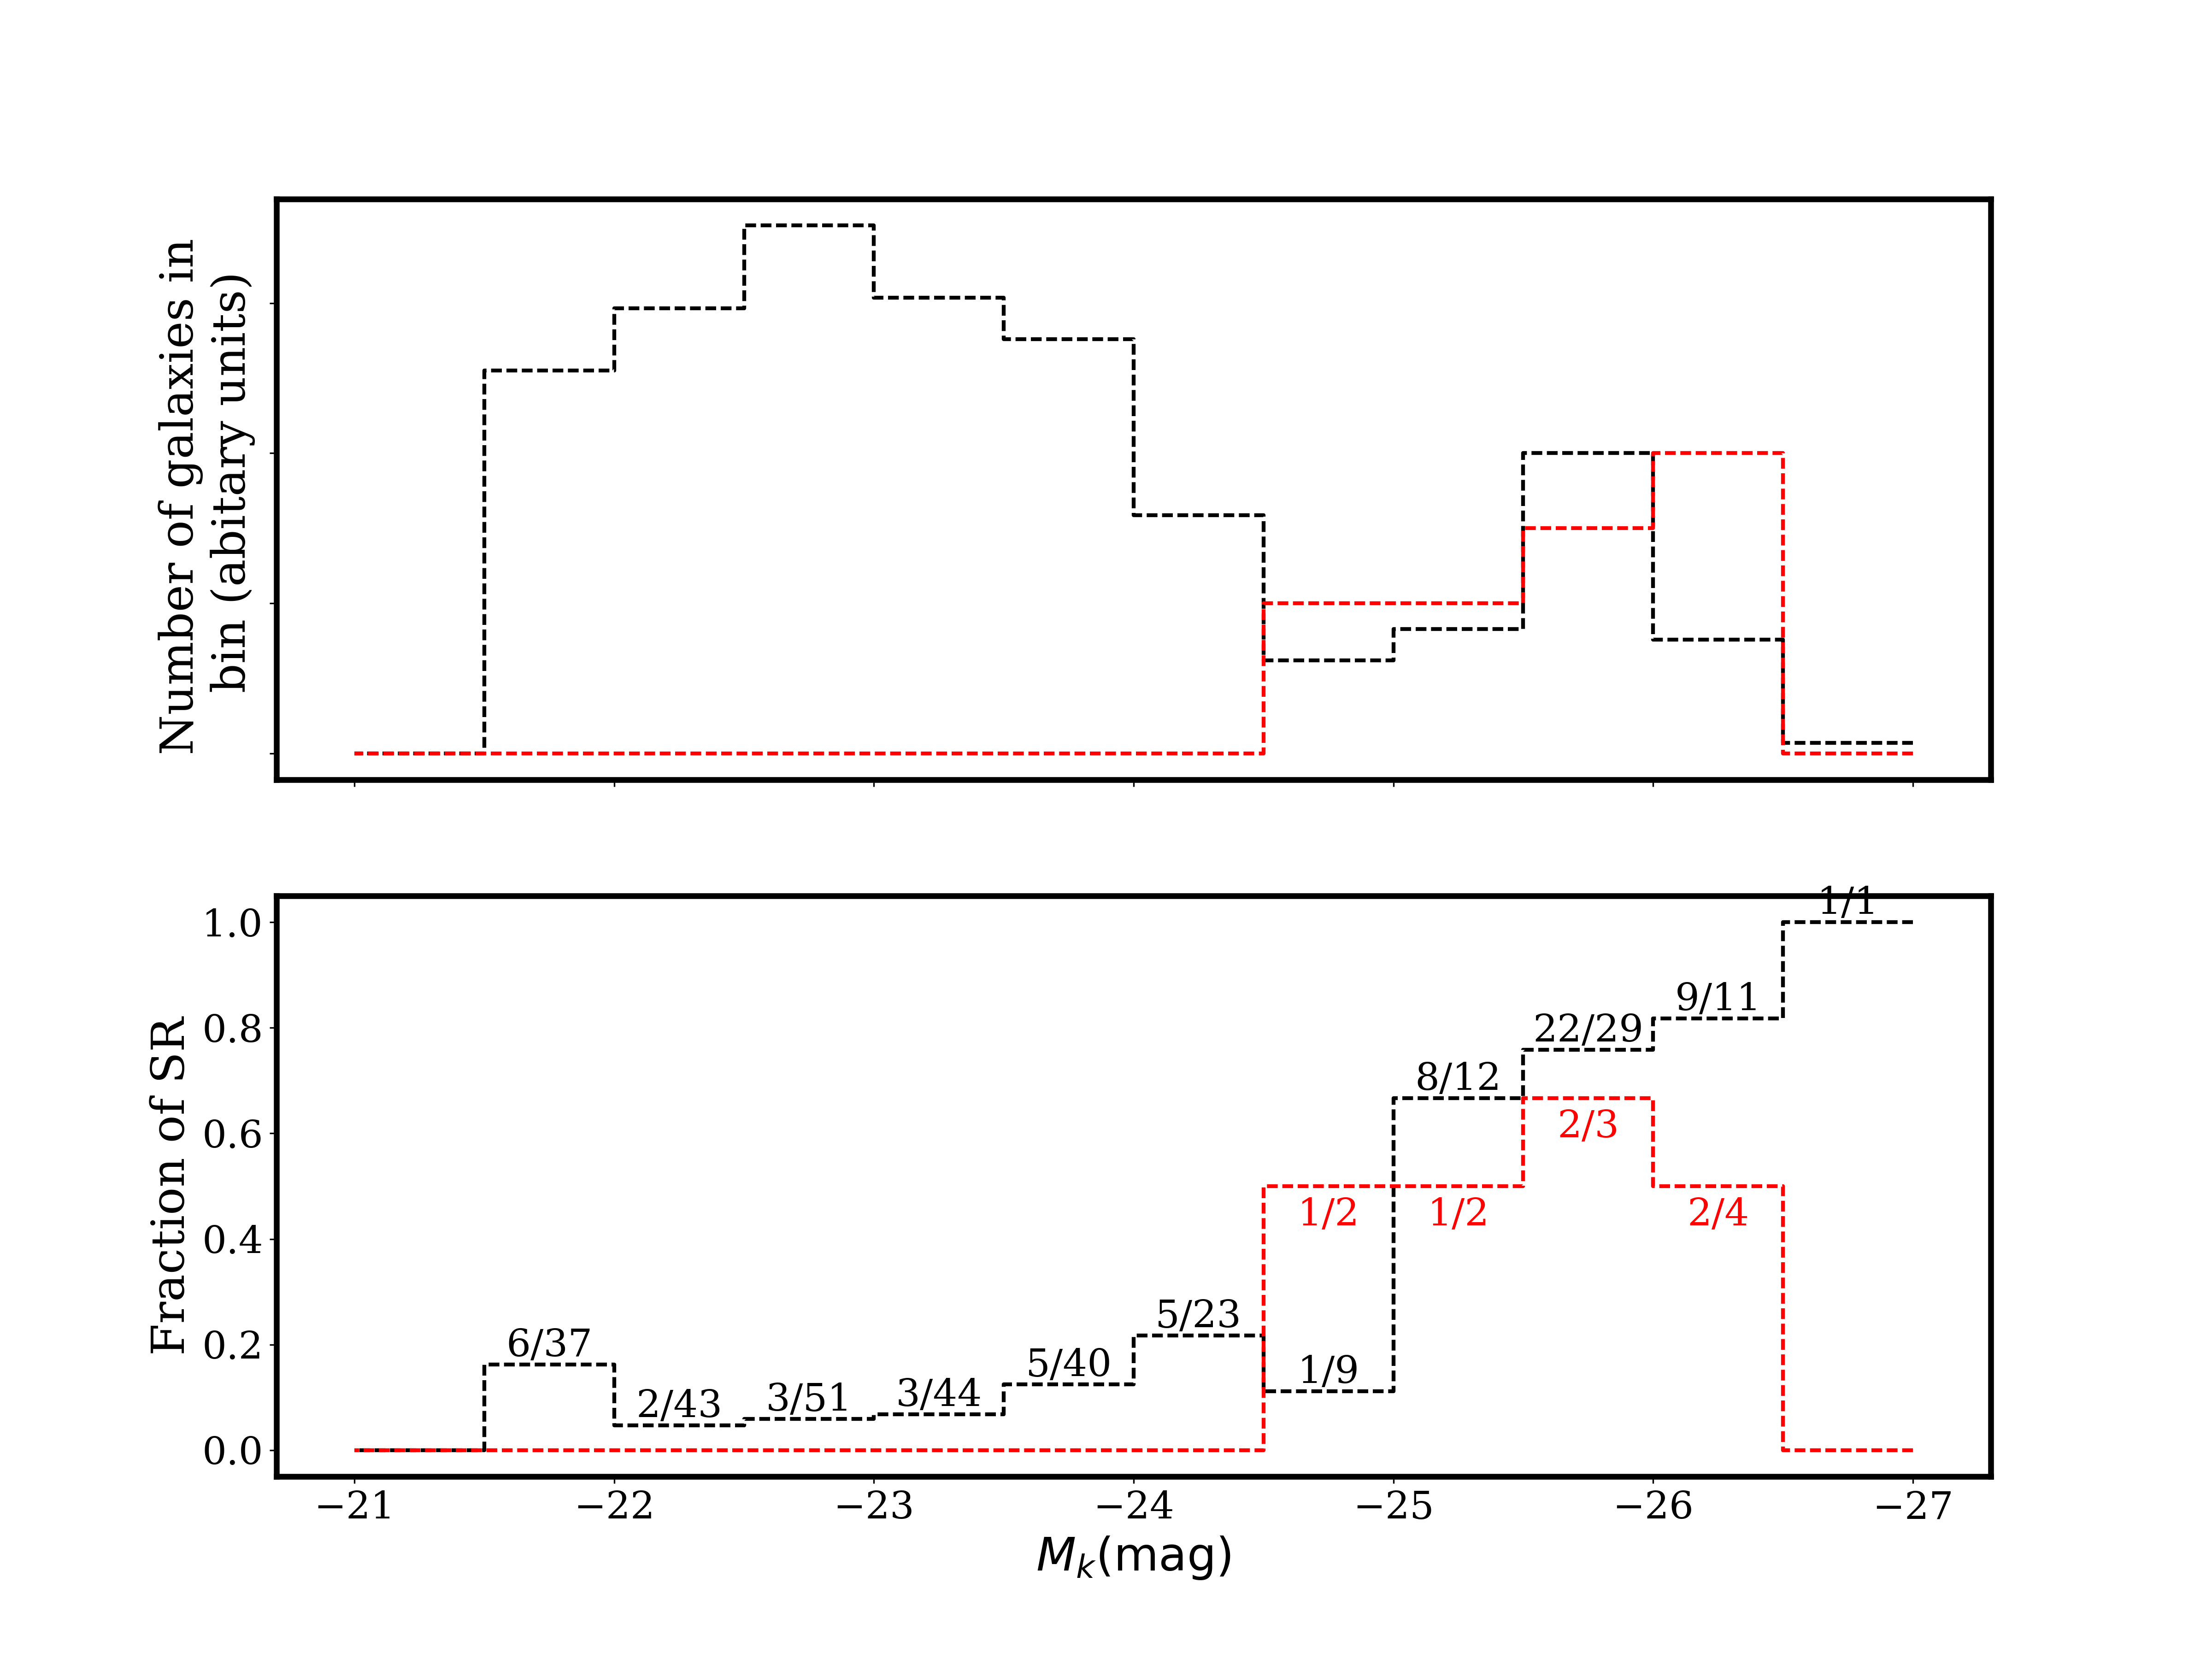
\includegraphics[width=0.8\textwidth]{chapter4/M_k_binned.png}
			\caption[Mass matching global kinematics]{Upper panel: mass distribution of the A+M sample (black) and of our Southern sample (red). Lower panel: fraction of slow rotators within each mass bin. The labels list the number of slow rotators and total number of galaxies in each bin.}
			\label{fig:SRmassFraction}
		\end{figure}

	\subsection{Radial Angular Momentum Profile}
		\label{subsec:ResolvedLambda_R}
		The radial $\lambda_R$ profiles (i.e.\ $\lambda_R$ as a function of aperture radius) are shown in Fig.\,\ref{fig:lambdaR_profile}. We see, with the exception of IC 1531, a disc with very low inclination, fast and slow rotators are separated by $\approx 0.3\,\mathrm{R_\odot}$. We also see that most of the fast rotators of our Southern sample have a rapidly rising $\lambda_R$ profile, which flatten out by $\approx 0.5\,\mathrm{R_\odot}$. This is consistent with the SAURON surveys findings \citep[e.g.][Fig.\,2]{Emsellem2007}. 

		\begin{figure}
			\centering
			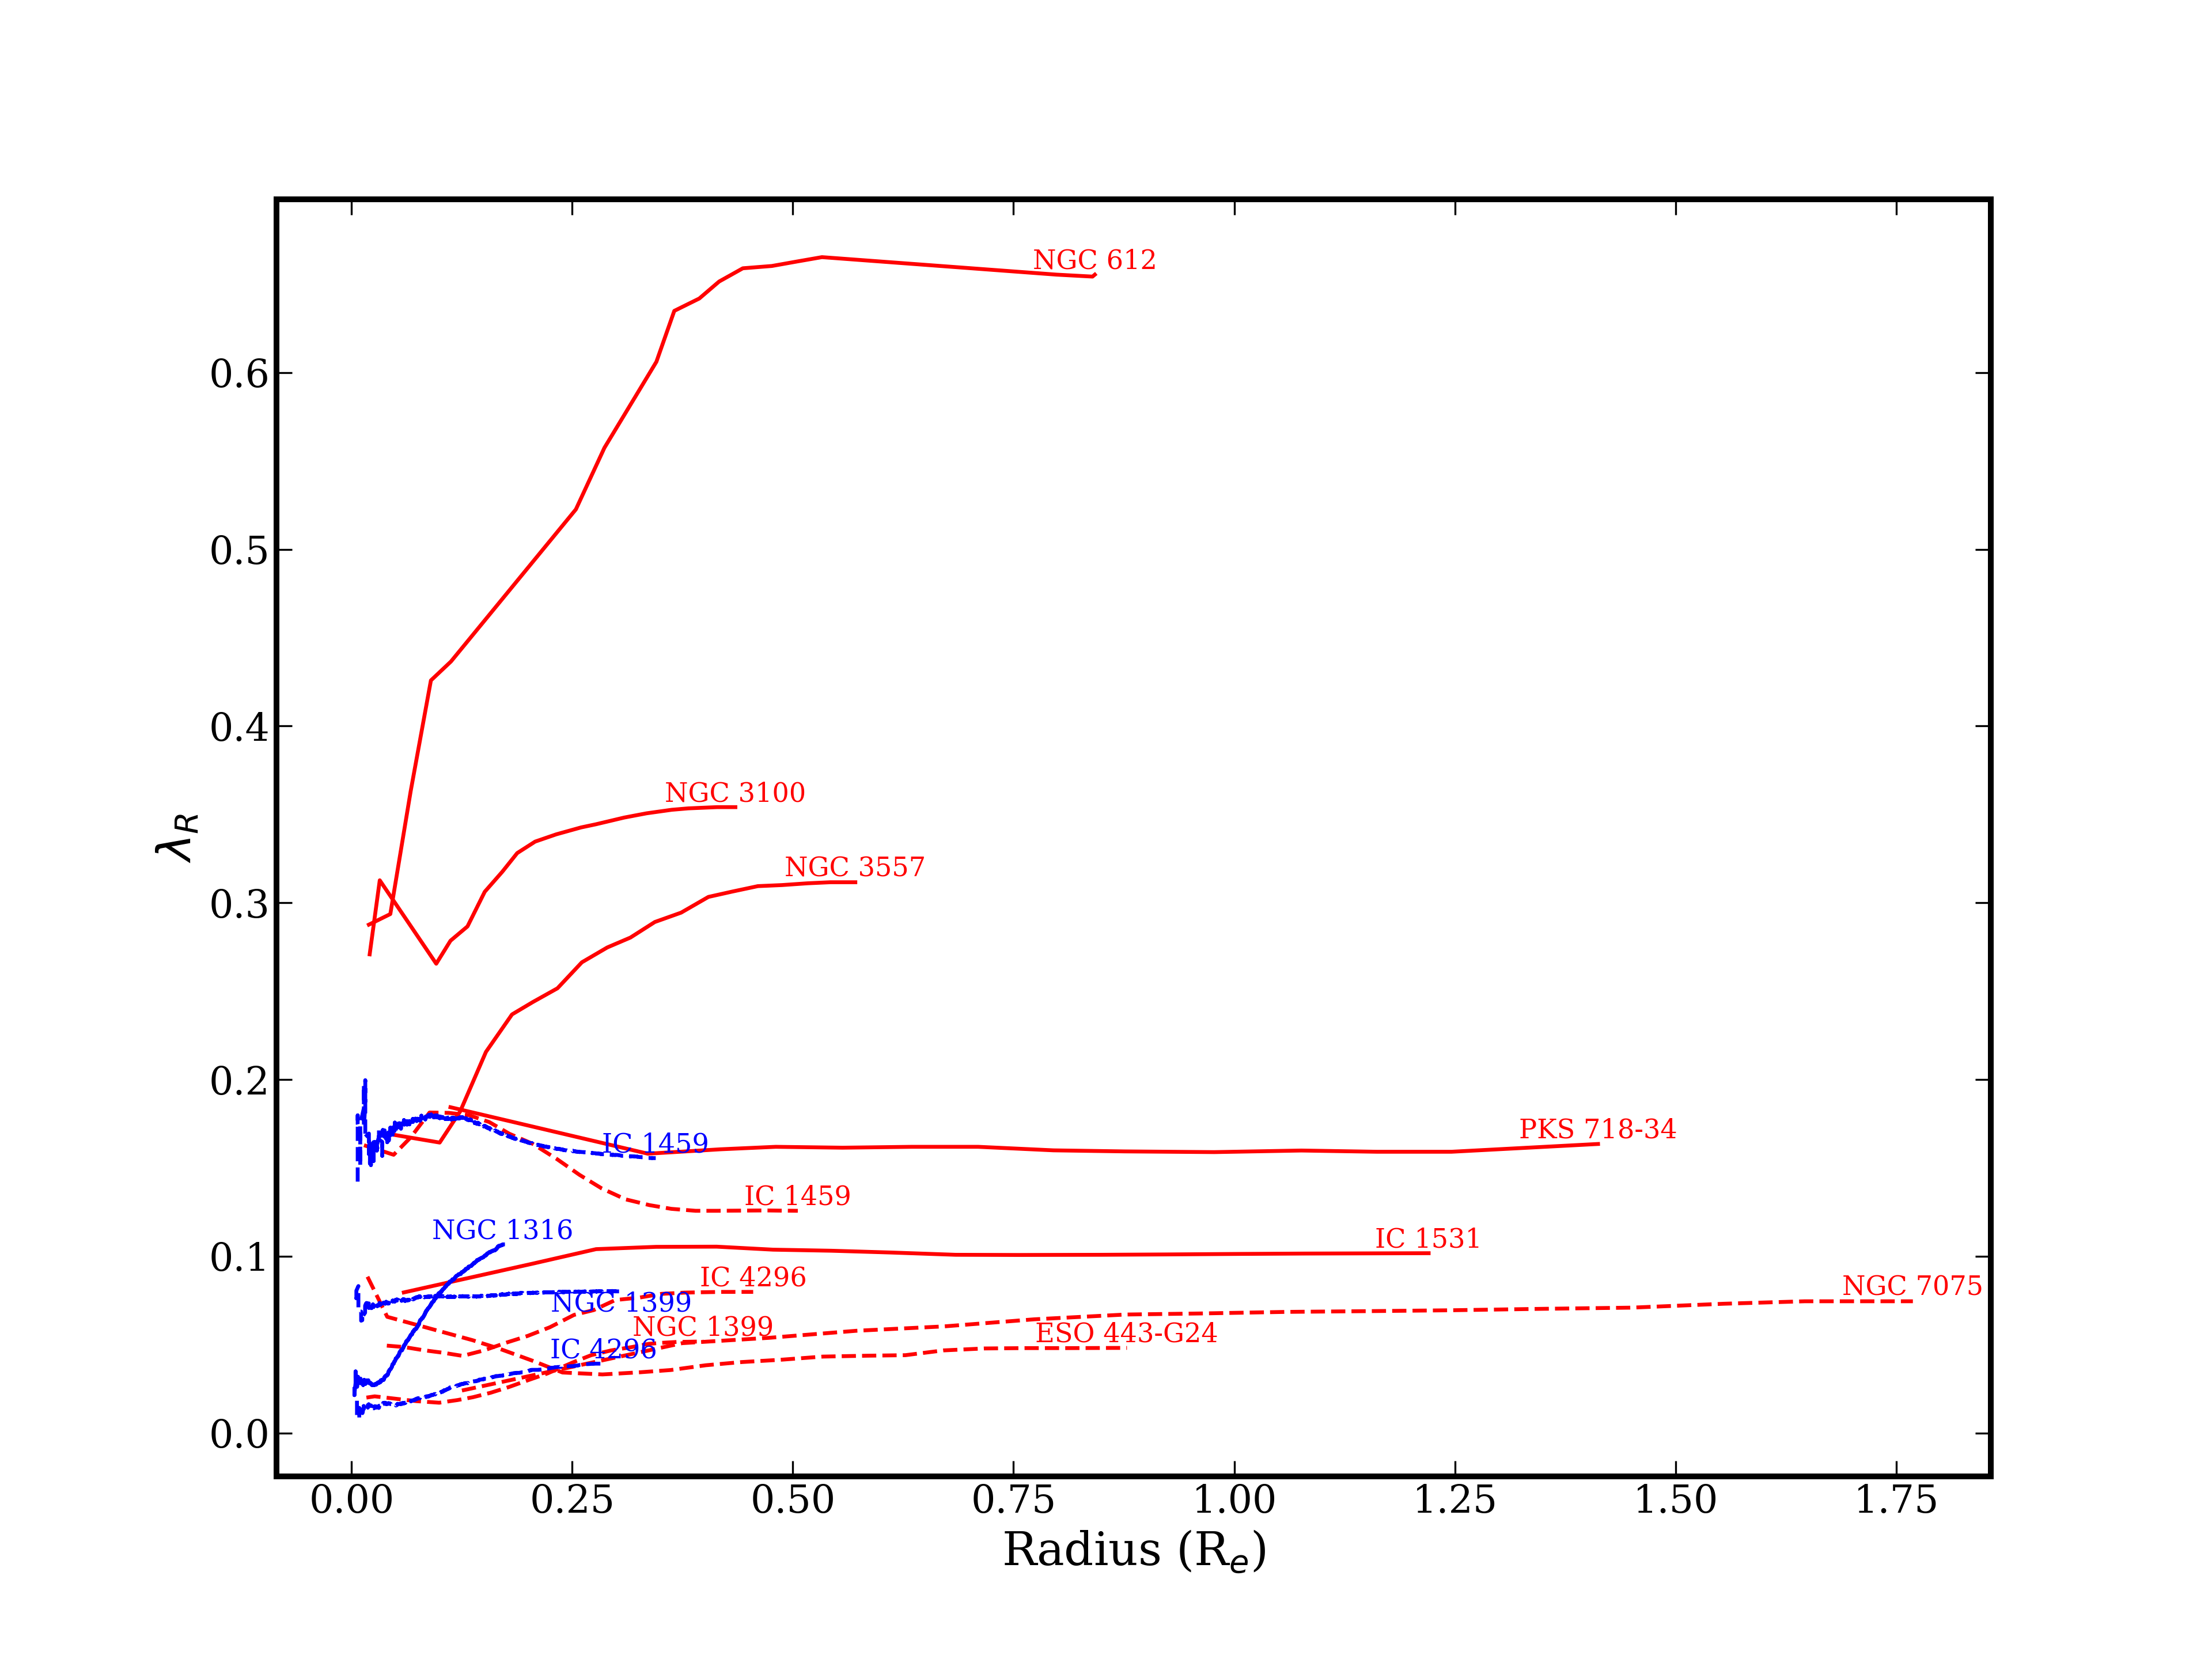
\includegraphics[width=.7\textwidth]{chapter4/lambda_R.png}
			\caption[$\lambda_{R}$ radial profiles]{Radial $\lambda_{R}$ profiles. Profiles derived from VIMOS data are in blue, while those derived from MUSE data are in red. Solid lines represent fast rotators; dashed lines, slow rotators.}
			\label{fig:lambdaR_profile}
		\end{figure}

		
		\subsection{Intrinsic Shape}
			\label{subsec:Misalignment}

			The photometric position angle, $PA_\text{phot}$, is defined as the angle westwards from North of semi-major axis of the largest best-fitting ellipse as found in Section \ref{subsec:Ellipticity}. The kinematic position angle, $PA_\text{kin}$, is defined as the angle of the axis perpendicular to the apparent angular momentum vector westwards from North. A global value of $PA_\text{kin}$ is found using the \textsc{python} routine \textsc{fit\_kinematic\_pa}\footnote{\url{http://www-astro.physics.ox.ac.uk/\~mxc/software/\#pa\_kin}} as described in appendix C of \citet{Krajnovic2006}. This routine finds a symmetric (about $PA_\text{kin}$) velocity field, by replacing the mean velocity, $V$, in each bin with
			\begin{equation}
				V'(x, y) = \frac{V(x,y) + V(x, -y) - V(-x,y) - V(-x,-y))}{4} \,,
			\end{equation}
			where $x$ and $y$ are the centroid coordinates of a given bin, with the origin at the centre of the galaxy and the x axis aligned along $PA_\text{kin}$. Linear interpolation is used where necessary.

			Column 4 in Table \ref{tab:classify} lists the misalignments between the photometric and kinematic position angles, $\Gamma_\text{kin} \equiv \arcsin(\sin[PA_\text{phot} - PA_\text{kin}])$. Misaligned systems may appear aligned in certain projections (though aligned systems will be aligned in all projections) and as such $\Gamma_\text{kin}$ cannot be used to describe the intrinsic shape of an individual galaxy, but, as described in Section \ref{sec:ETG}, it can be used in a statistical manner as in \citet{Cappellari2007}. We find all the regular rotators in our Southern sample, are consistent with having aligned photometry and kinematic position angles to within 11\degree, while non-regular rotators have a large range of values of $\Gamma_\text{kin}$. IC 1531, NGC7075 and PKS 718-34 all have very large uncertainties in the value of $PA_\text{phot}$ due to the VIMOS quadrant artefacts causing the fitting routine of \textsc{kinemetry} to become unreliable. 

			The lack of misalignments in regular rotators is consistent with \citet{Cappellari2007}, \citet{Krajnovic2011} and \citet{Fogarty2015}, who all showed that regular rotators almost always have aligned photometric and kinematic axes with very little scatter and that regular rotators with a significant misalignment are either interacting or strongly barred. The lack of misalignments suggests that the regular rotators (including those within our Southern sample) are consistent with being axisymmetric \citep{Cappellari2016}.

			Misalignments between the photometric and kinematic position angles are routinely observed for non-regular rotators. This generally implies a more triaxial intrinsic shape, although large misalignments are extremely rarely observed in galaxies with $\epsilon > 0.4$, suggesting that non-regular rotators are more spherical in shape \citep{Cappellari2016}. The non-regular rotators in our Southern sample indeed all have $\epsilon < 0.4$ and a broad range of misalignment angles and are thus consistent with a fairly spherical, triaxial intrinsic shape.


\section{Stellar Population}
	\label{sec:pop}
	As described in Section \ref{subsec:PopFit}, in order to find the best-fitting stellar populations for our Southern sample, we must first measure the absorption line strengths of the indices in Table \ref{tab:abIndex}. We first present maps of the strength of each index (Section \ref{subsec:absorption}), before examining the Mg\,--\,$\sigma$ relation (Section \ref{subsubssec:Mgsigma}), comparing the measured line strengths to the literature (Section \ref{subsubsec:Lit}) and finally presenting maps of the stellar populations (Section \ref{subsec:ssp}).

	\subsection{Absorption Line Strengths}
		\label{subsec:absorption}

		Figs.\,\ref{fig:VIMOS_absorption} and \ref{fig:MUSE_absorption} show the spatially-resolved absorption line strengths of our Southern sample galaxies. For the VIMOS datacubes, we measure the G4300, Fe4383, Ca4455, Fe4531, H\,$\beta$, Fe5015 and Mg\,b indices, as defined in Table \ref{tab:abIndex}. For the most distant galaxies (NGC 612 and PKS 718-34), the red continuum band of the Mg\,b is redshifted beyond the spectral range of the VIMOS spectrograph. In these cases we have not attempted to adjust the definition of the Mg\,b index bandpass (as \citealt{Kuntschner2006} did with defining Fe5270s to use instead of Fe5270), but have simply not included Mg\,b in any future analysis of these galaxies. For the MUSE datacubes, we measure the H\,$\beta$, Fe5015, Mg\,b, Fe5270, Fe5335, Fe5406, Fe5709, Fe5782, NaD, TiO1 and TiO2 indices, also defined in Table \ref{tab:abIndex}.

		\begin{figure}
			\centering
			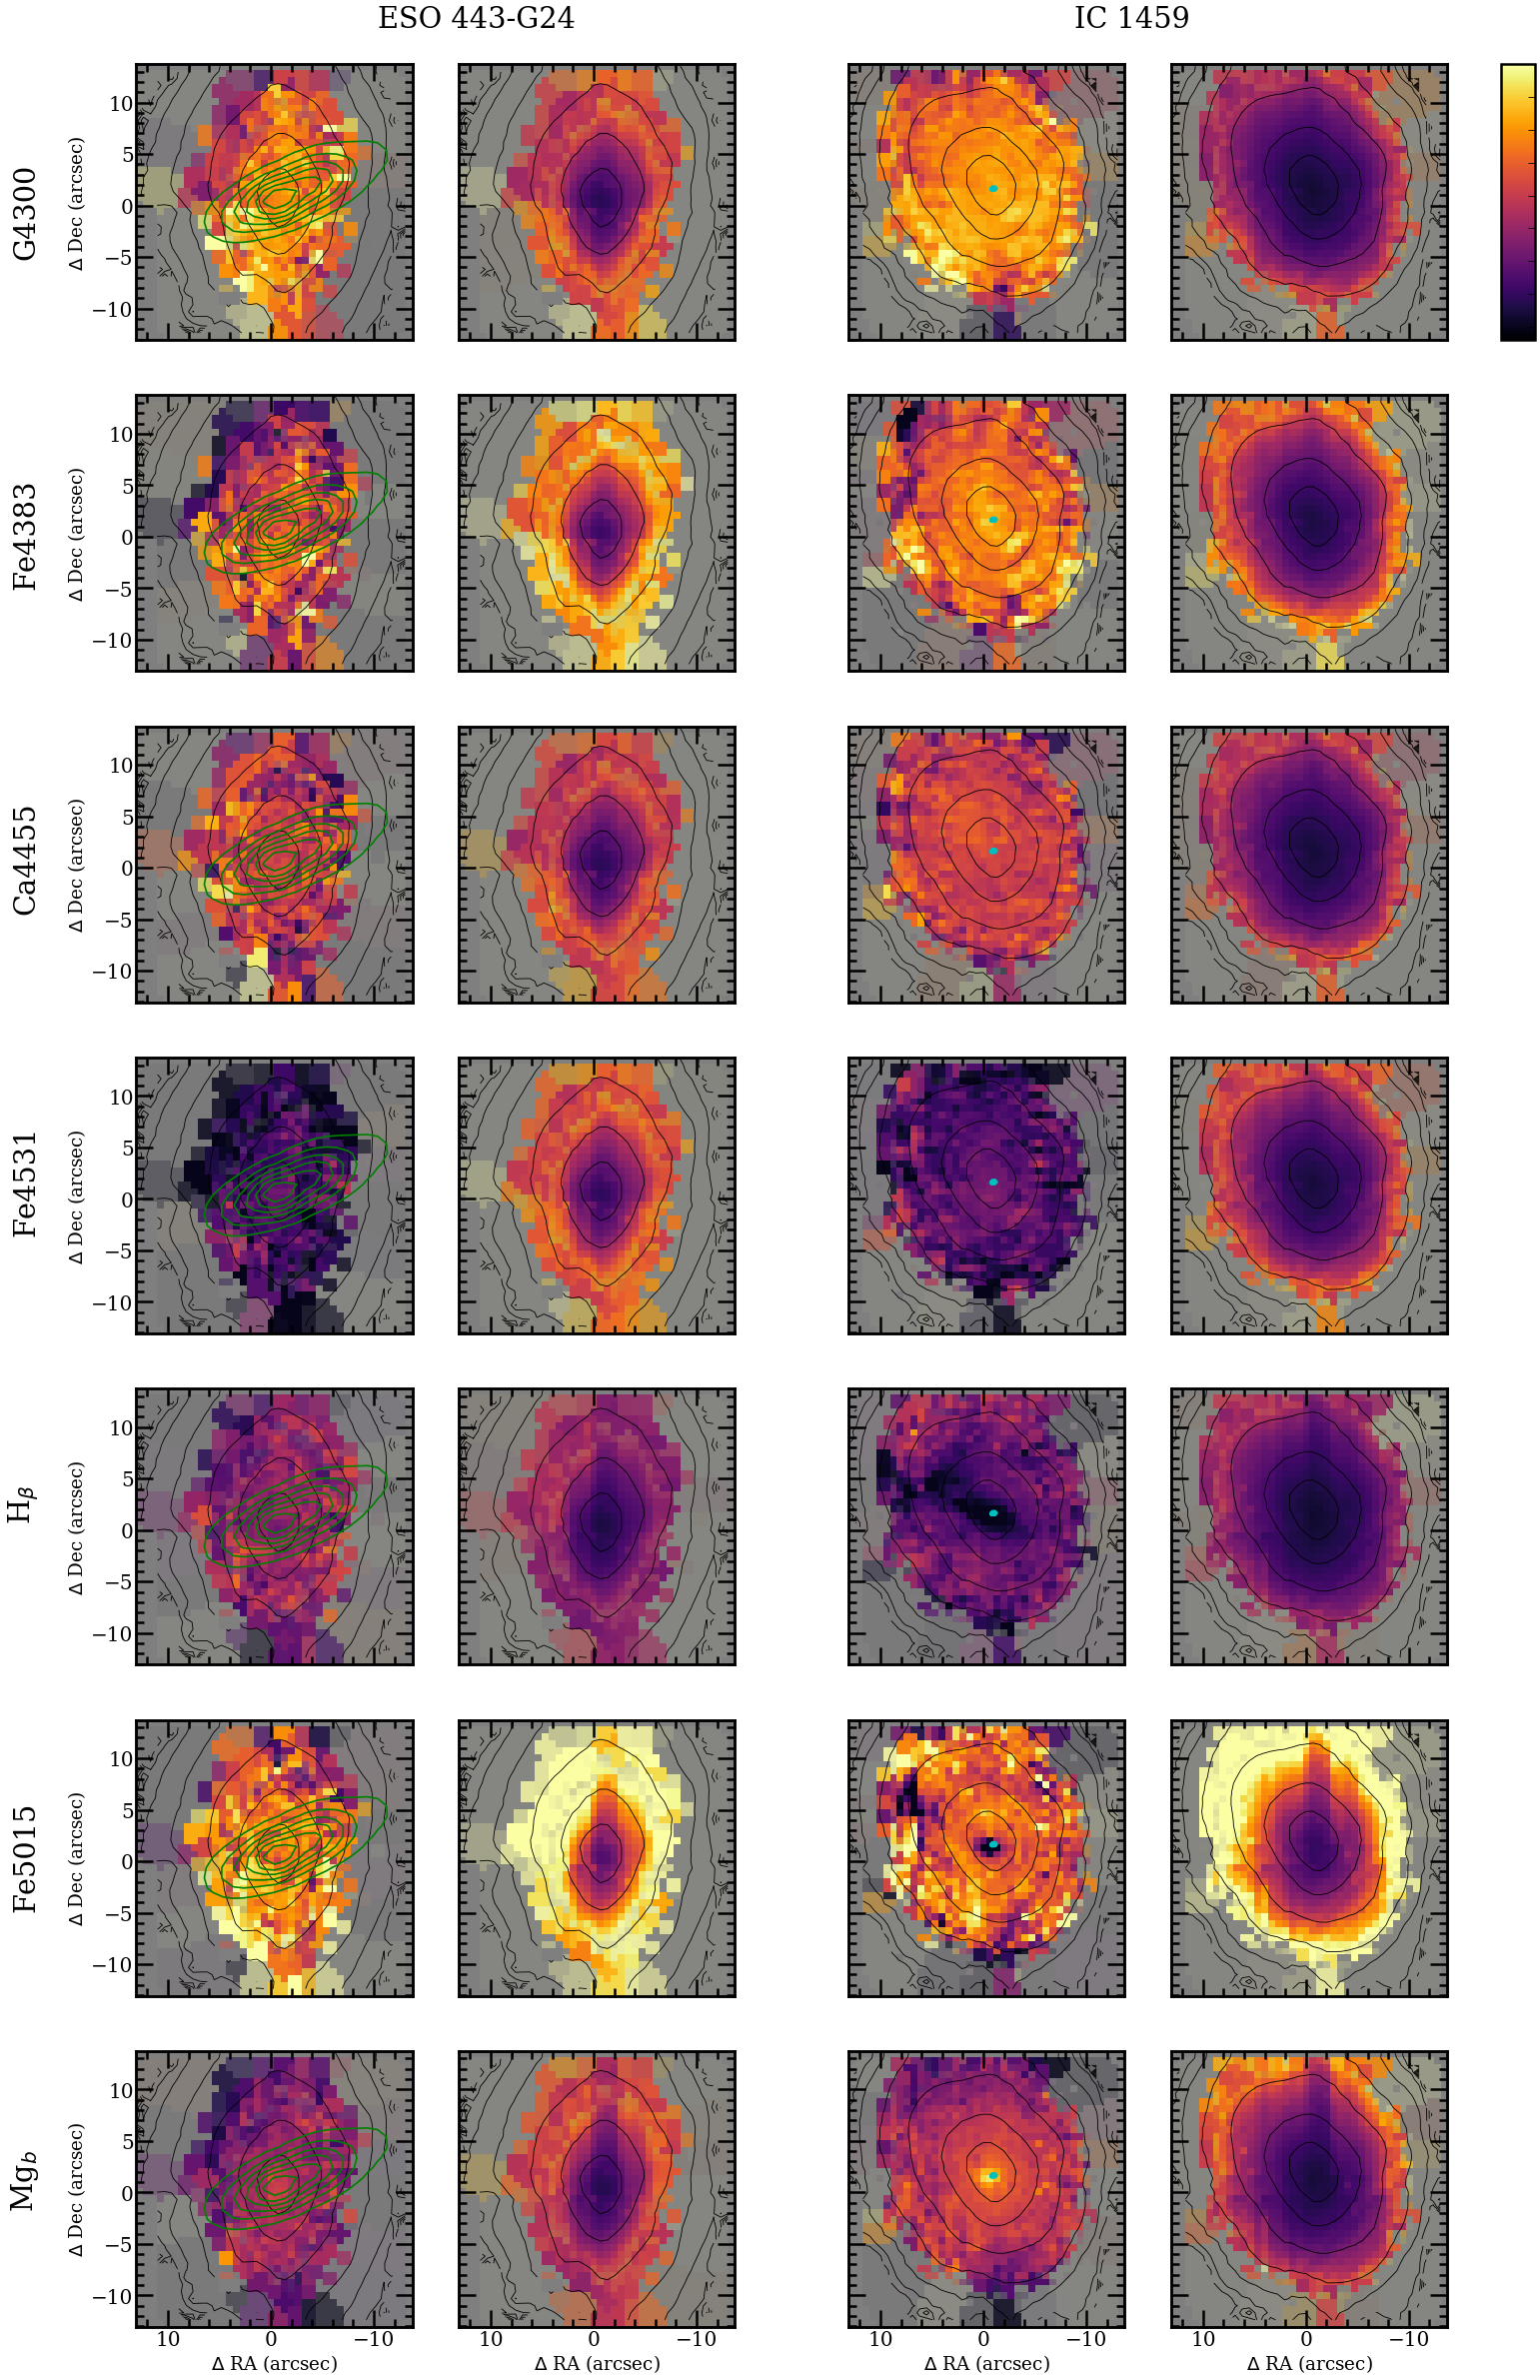
\includegraphics[height=0.89\textheight]{chapter4/vimos/abs1.png}
			\caption[VIMOS absorption line strength maps]{VIMOS absorption line strength maps. Left to right: ESO 443-G24 line index and associated uncertainties, IC 1459 line index and associated uncertainties. Top to bottom: G4300, Fe4383, Ca4455, Fe4531, H\,$\beta$, Fe5015 and Mg\,b index. contours are as in Fig.\,\ref{fig:VIMOS_stellar}. Limits on the colour scales are 0.5--3.5\,\AA\ for Ca4455 and H\,$\beta$ line strengths, 3--7\,\AA\ for all other line strengths and 0--0.5\,\AA\ for all uncertainty maps.}
			\label{fig:VIMOS_absorption}
		\end{figure}
		\begin{figure}
			\centering
			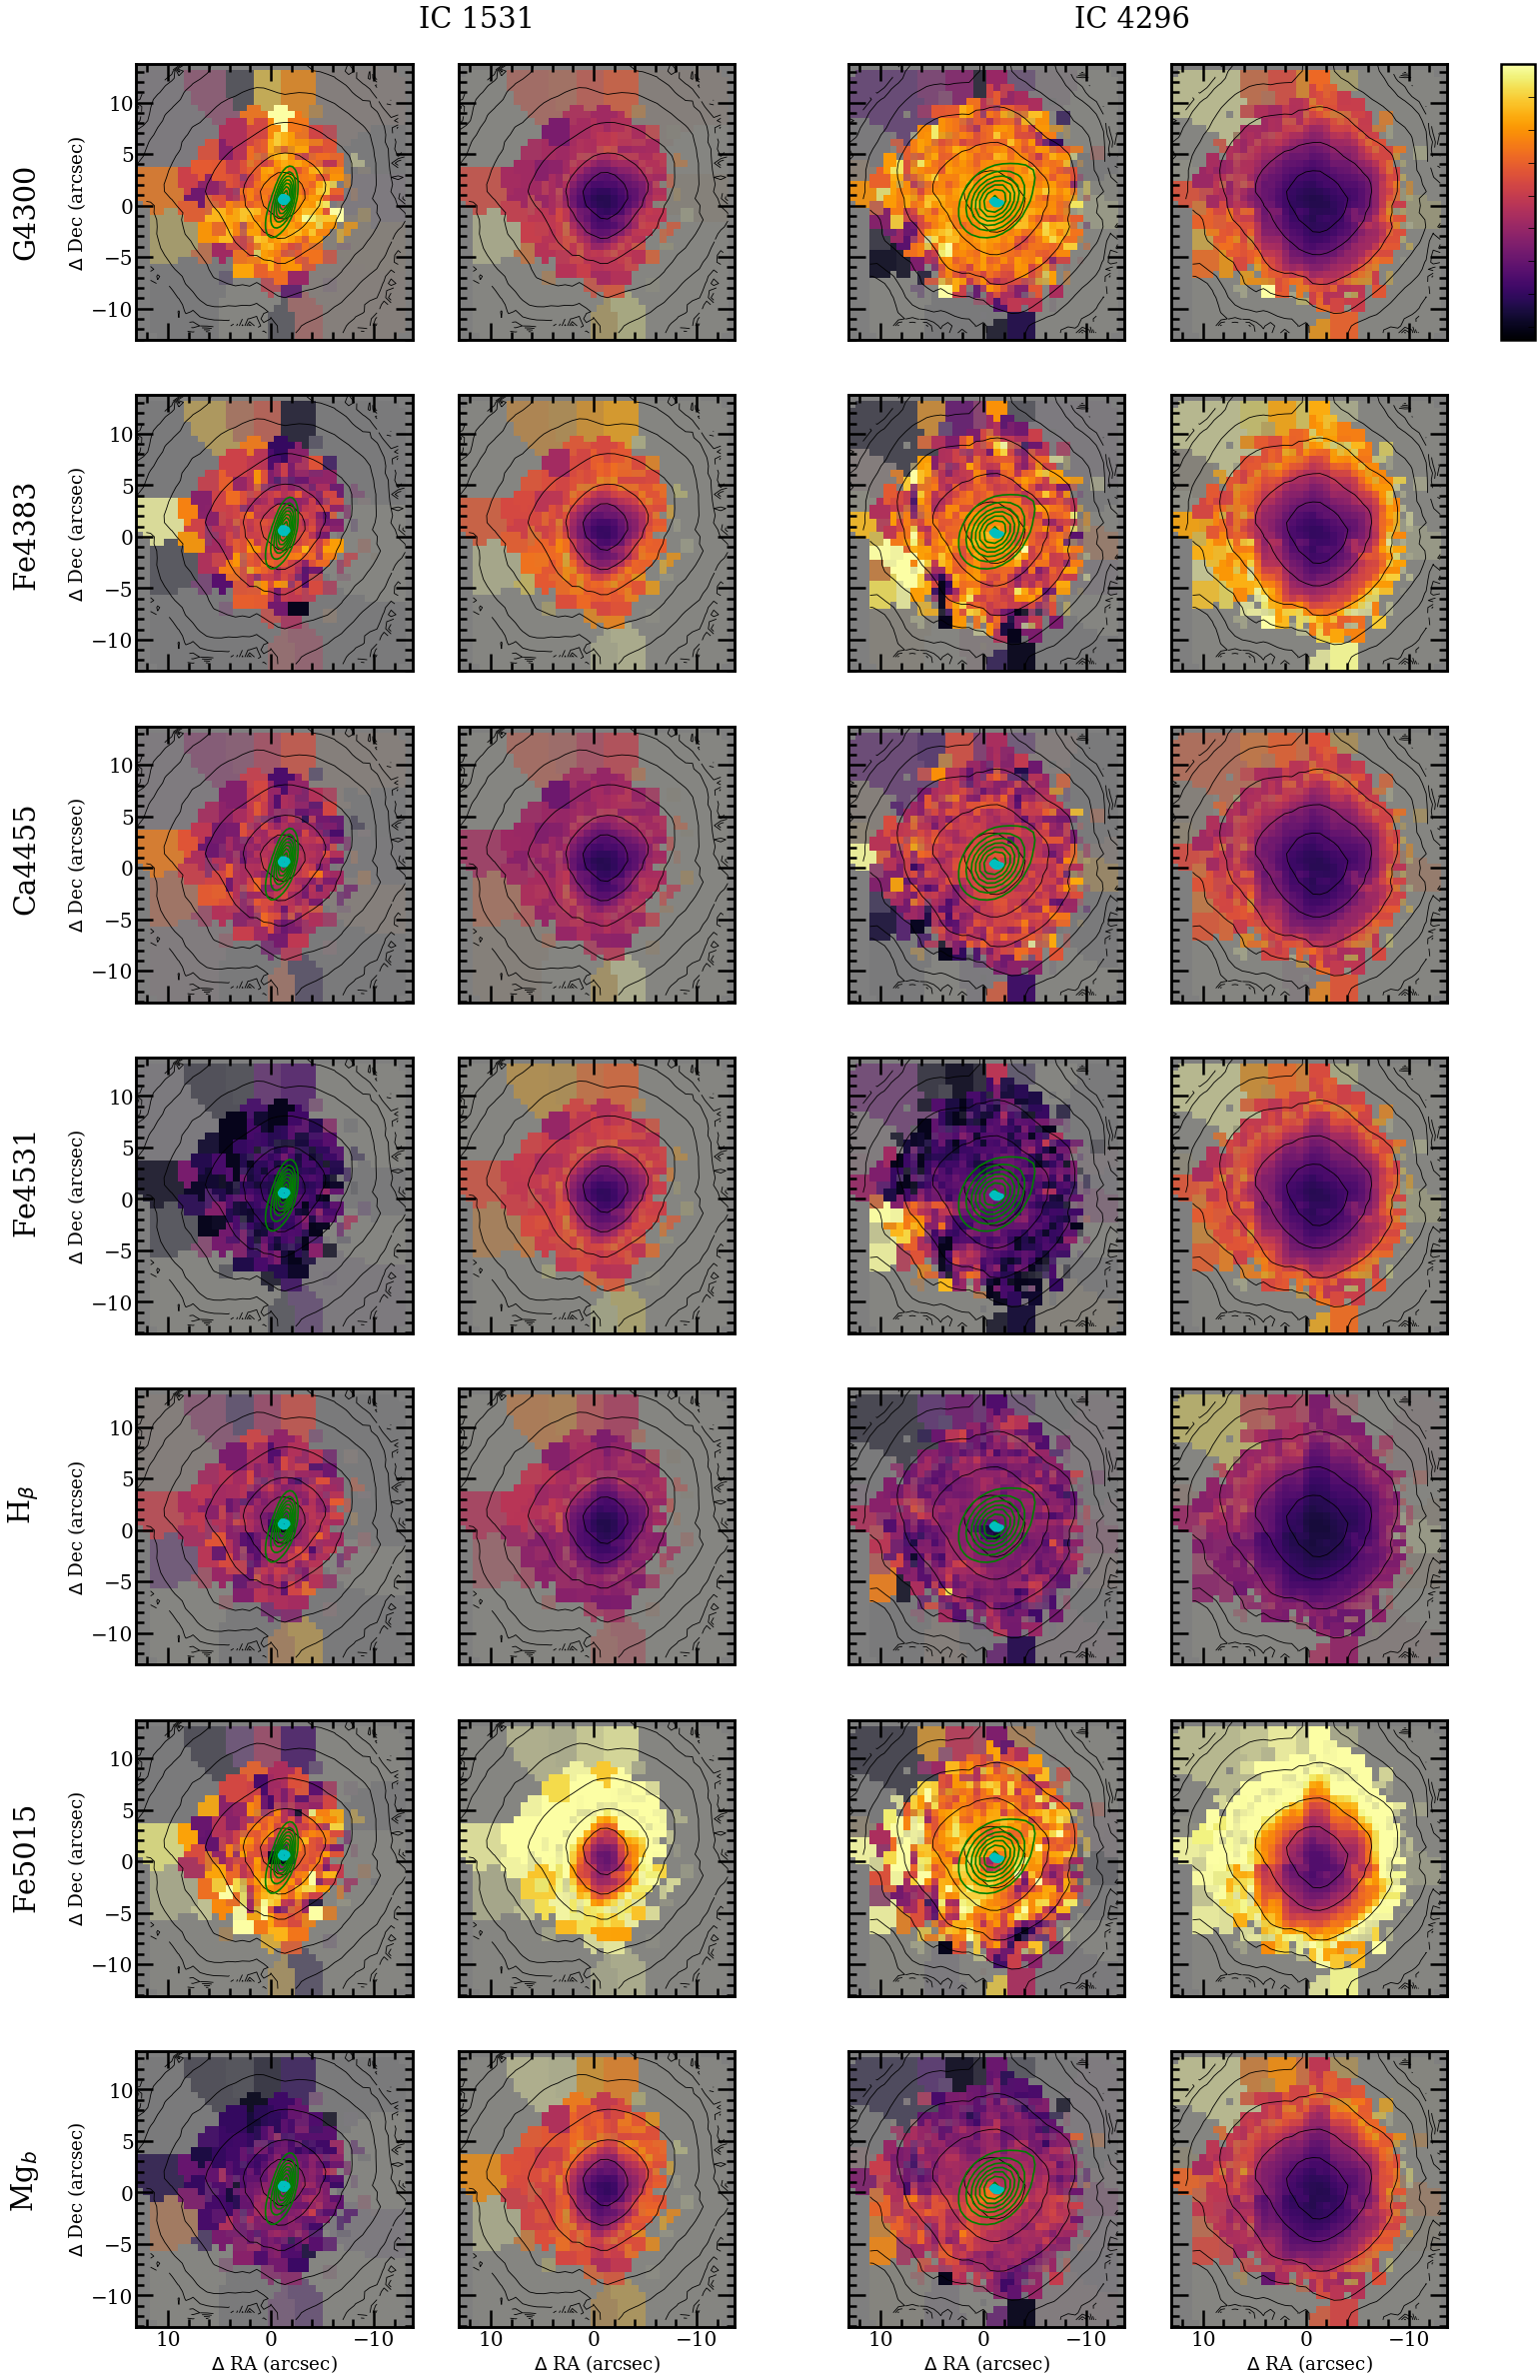
\includegraphics[height=0.94\textheight]{chapter4/vimos/abs2.png}
			\contcaption{\textit{Continued.}}% for IC 1531 and IC 4296.}
		\end{figure}
		\begin{figure}
			\centering
			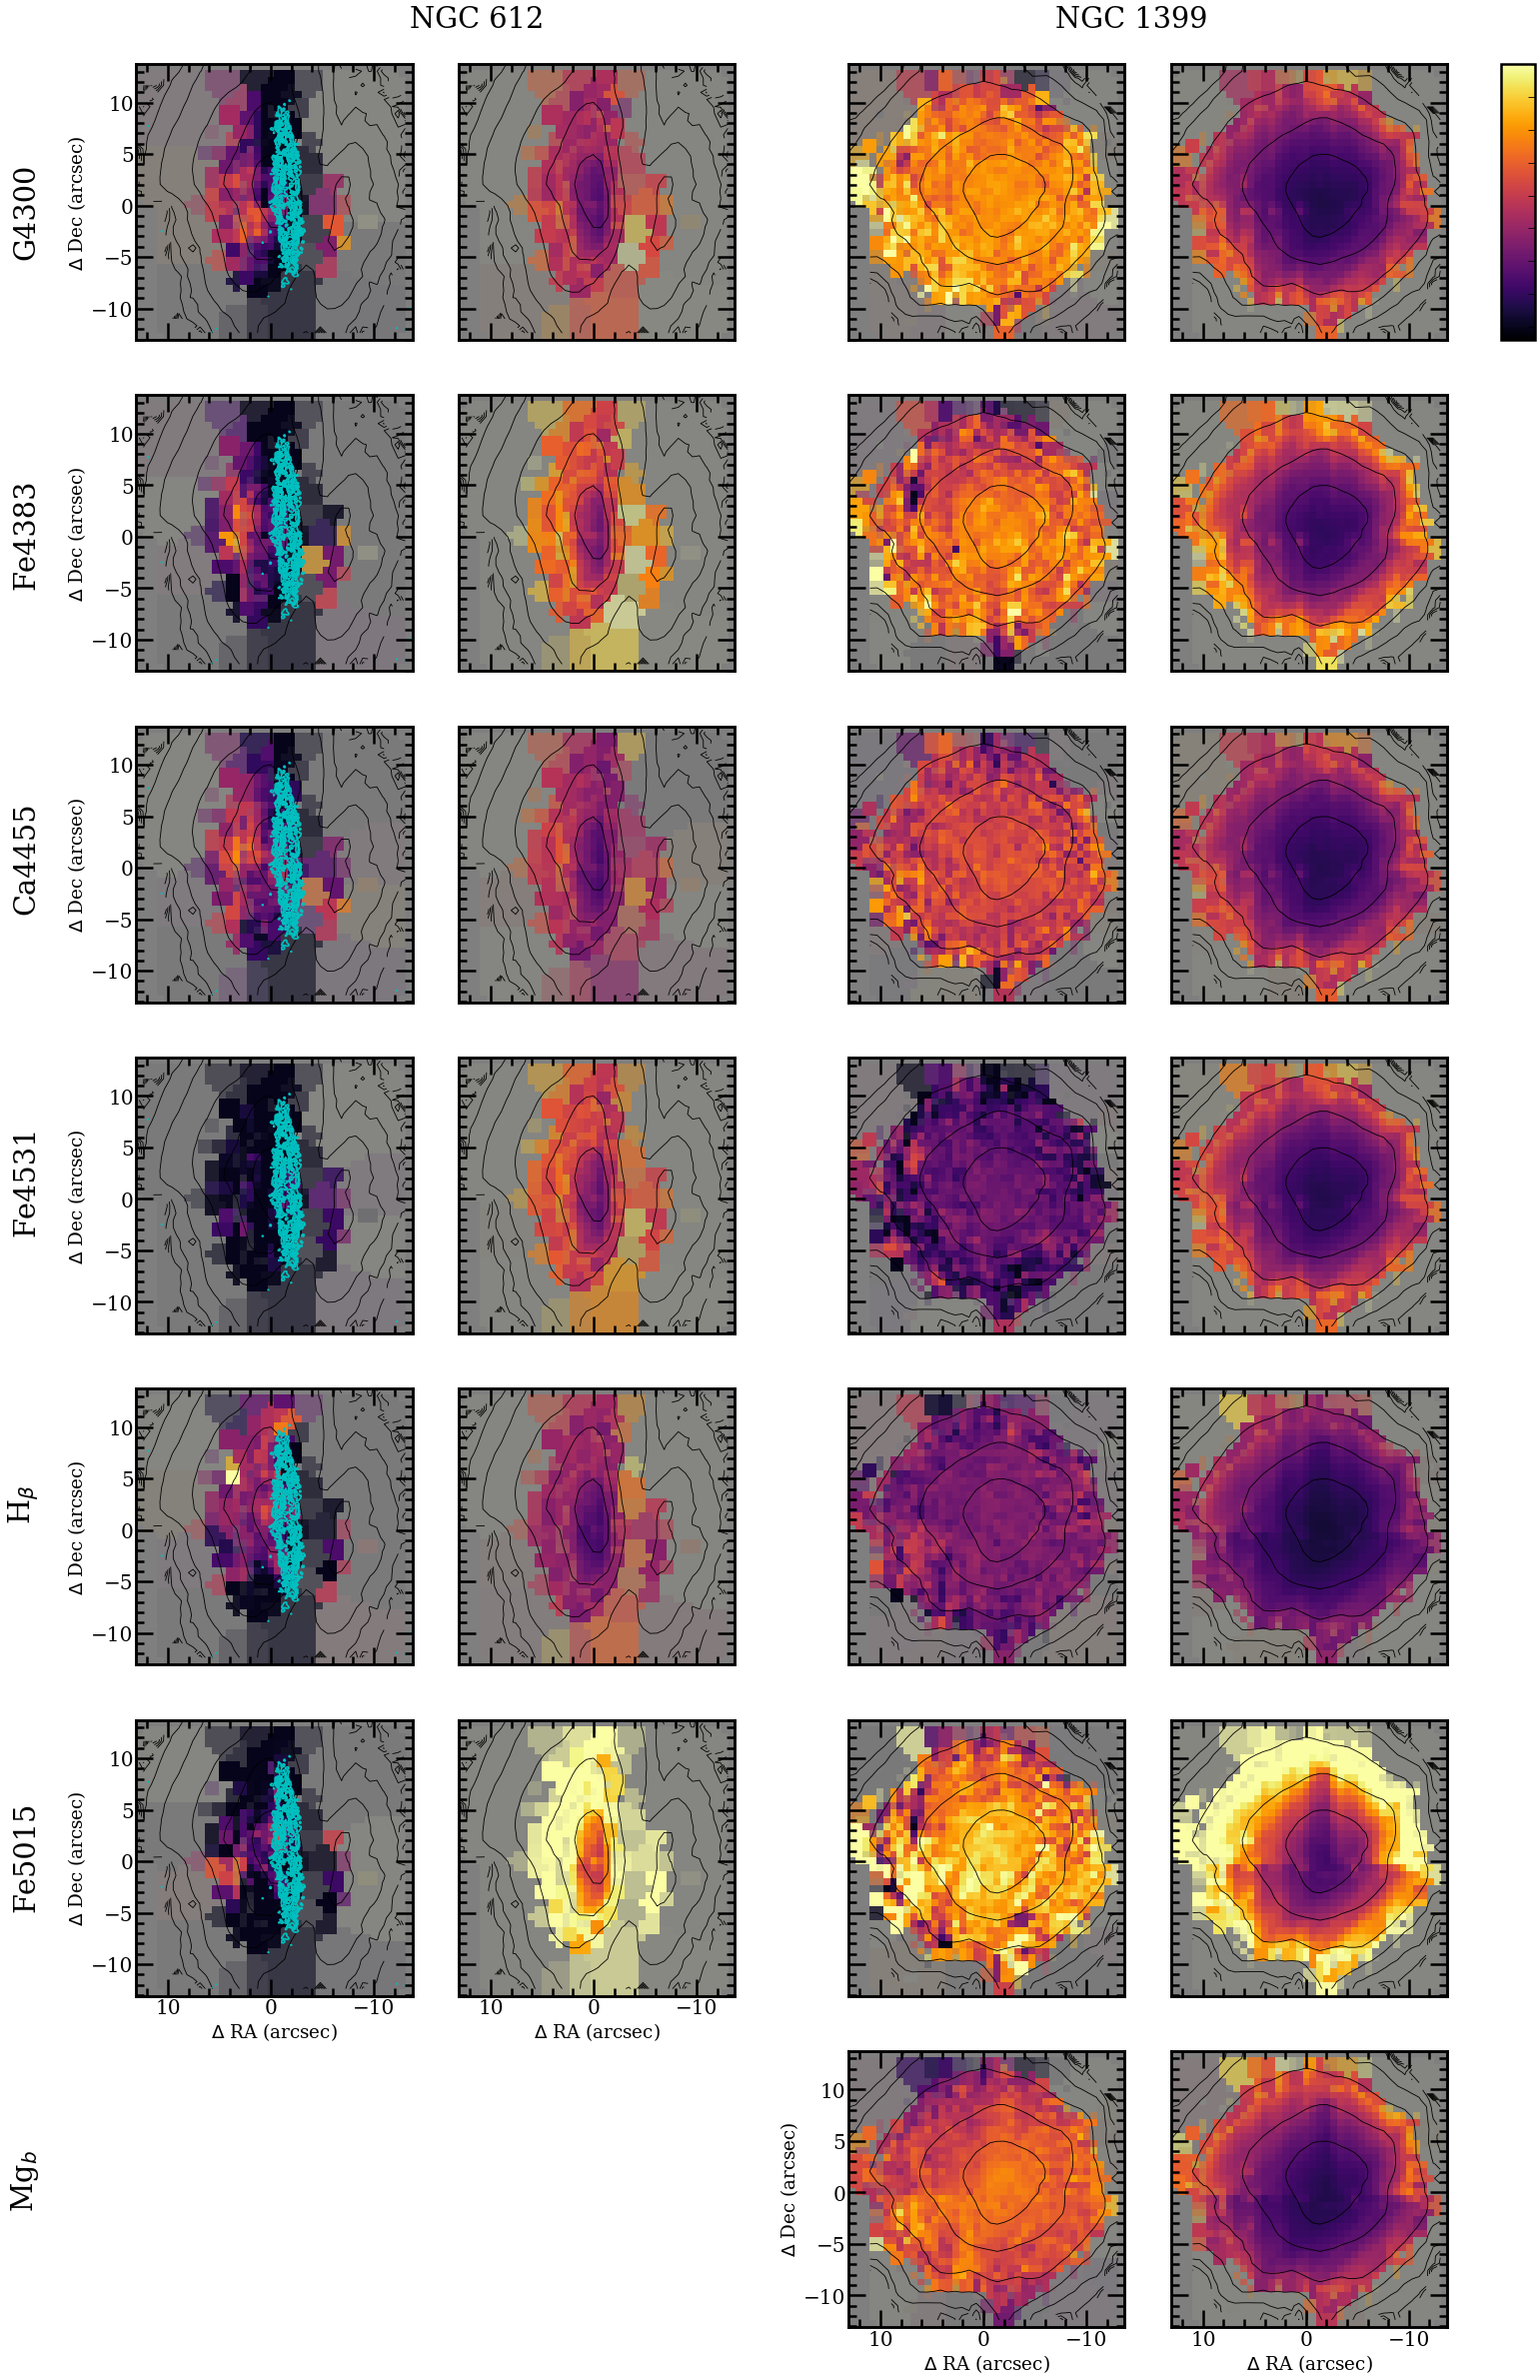
\includegraphics[height=0.94\textheight]{chapter4/vimos/abs3.png}
			\contcaption{\textit{Continued.}}% for NGC 612 and NGC 1399}
		\end{figure}
		\begin{figure}
			\centering
			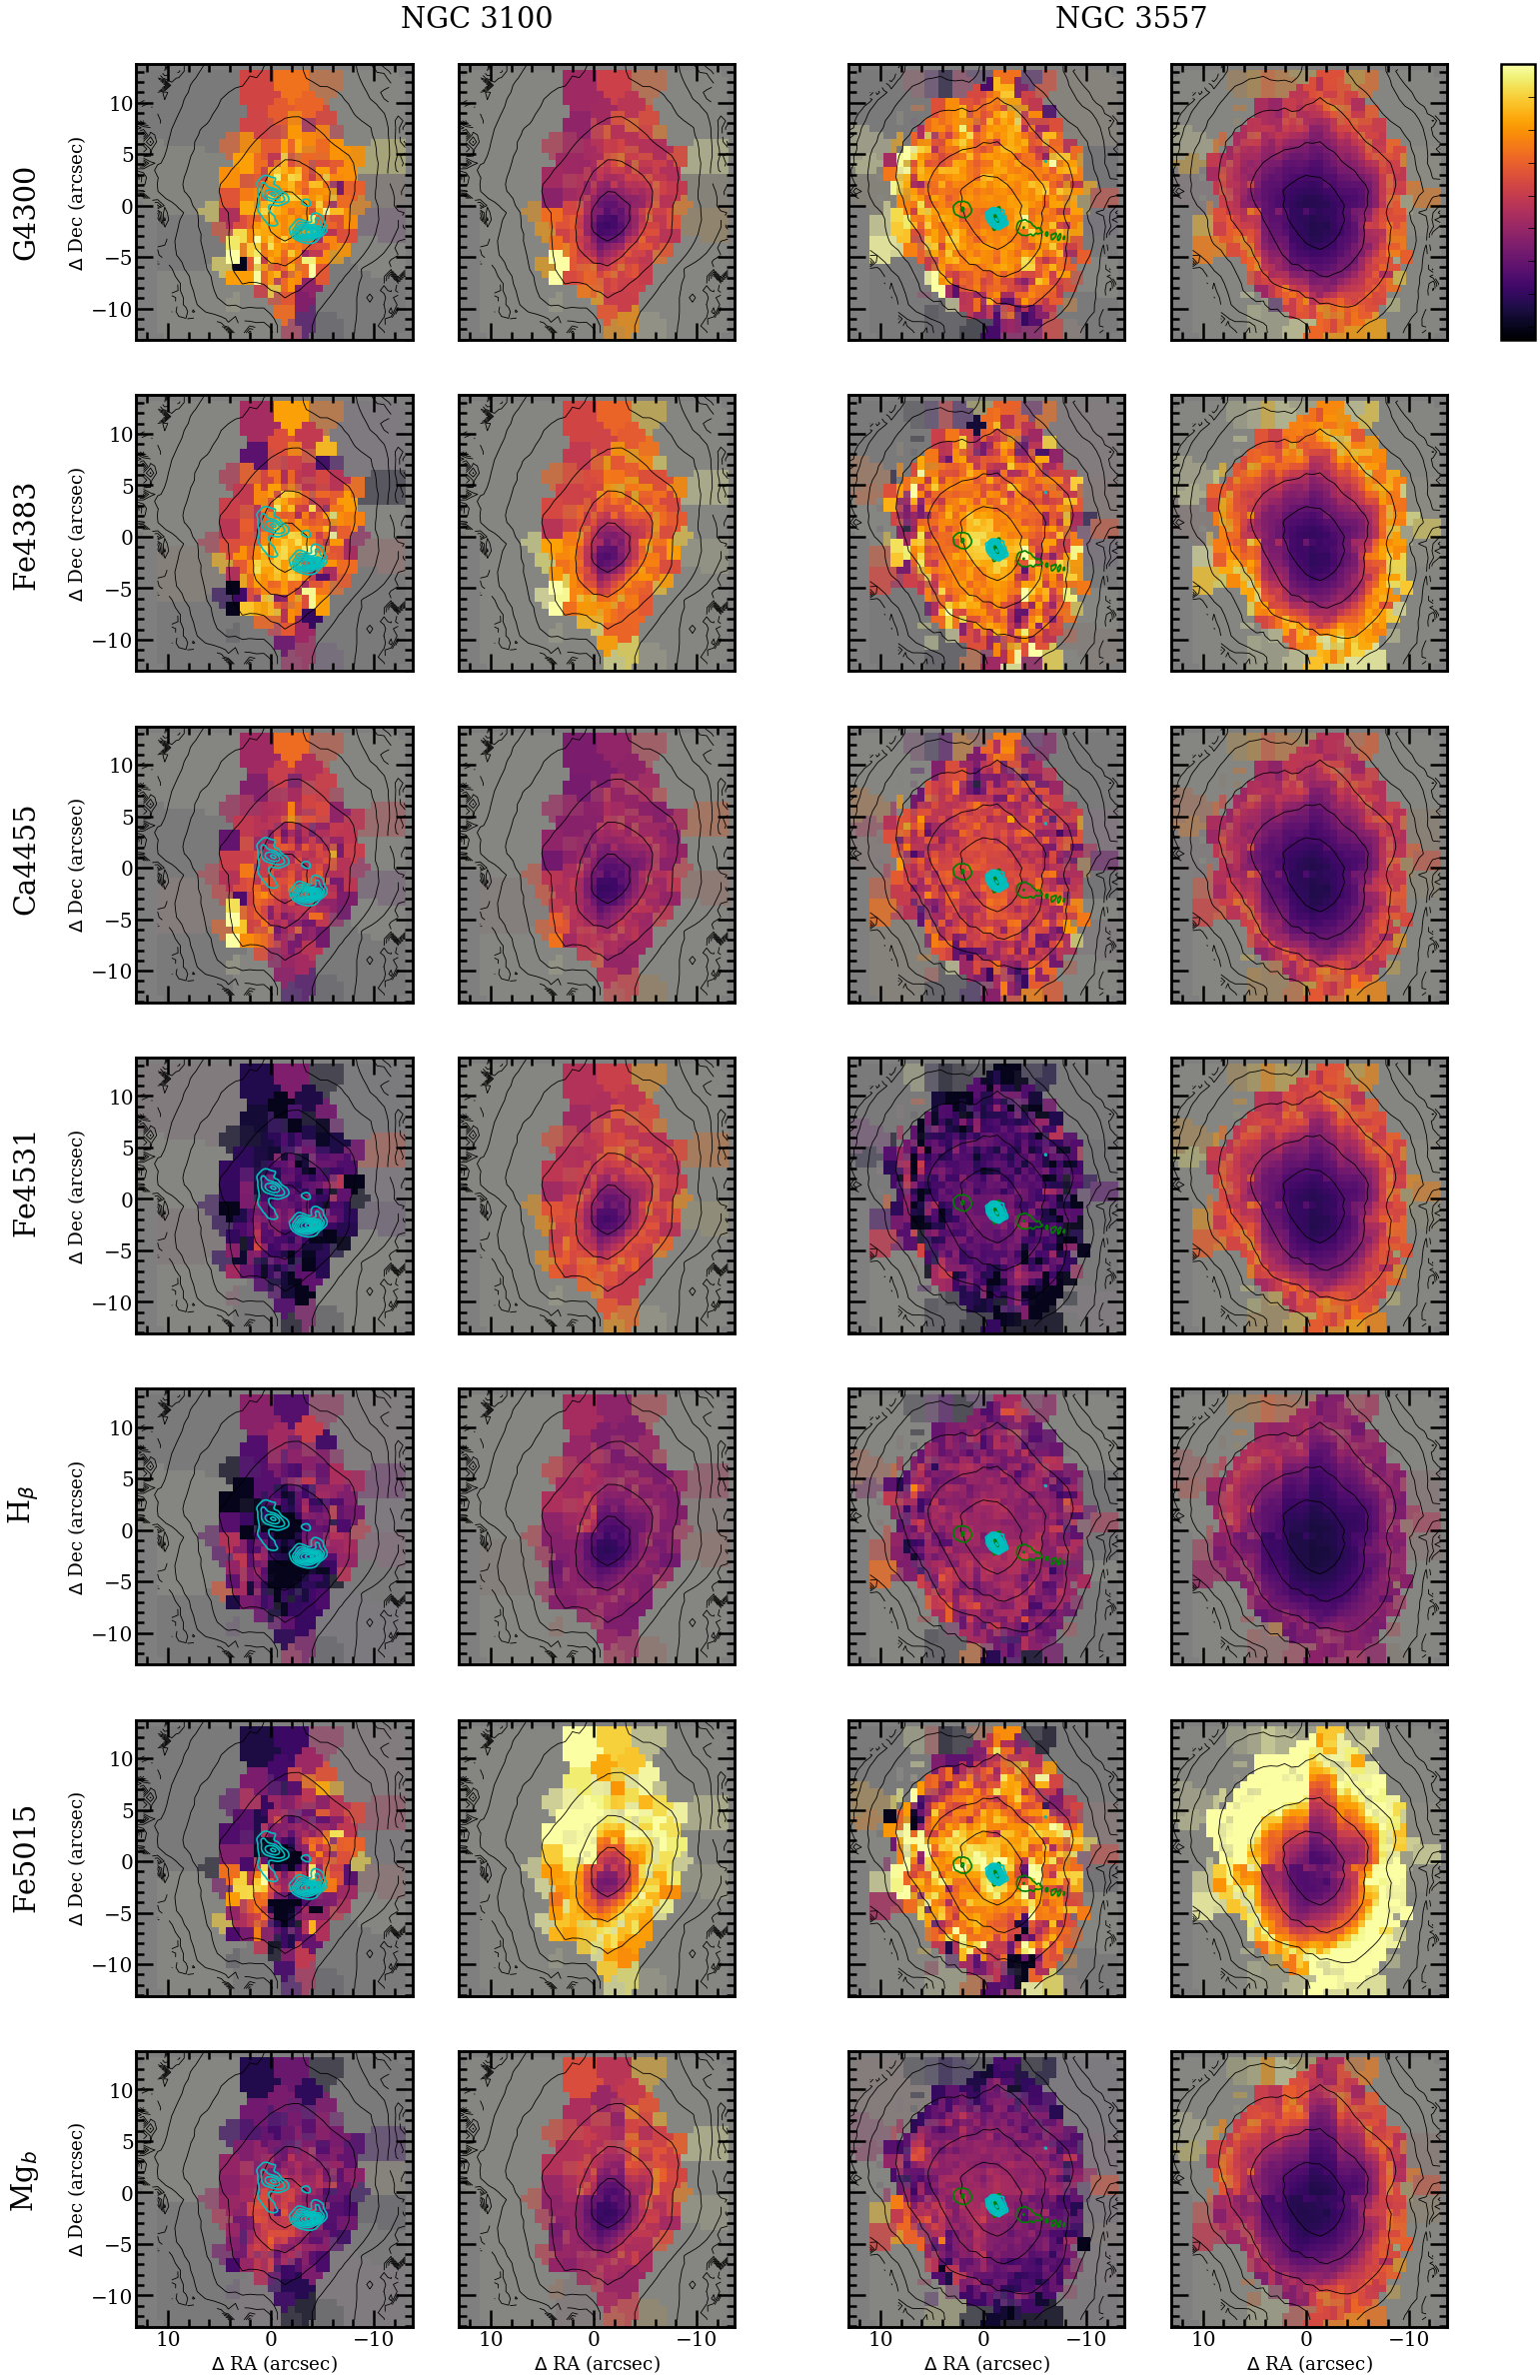
\includegraphics[height=0.94\textheight]{chapter4/vimos/abs4.png}
			\contcaption{\textit{Continued.}}% for NGC 3100 and NGC 3557}
		\end{figure}
		\begin{figure}
			\centering
			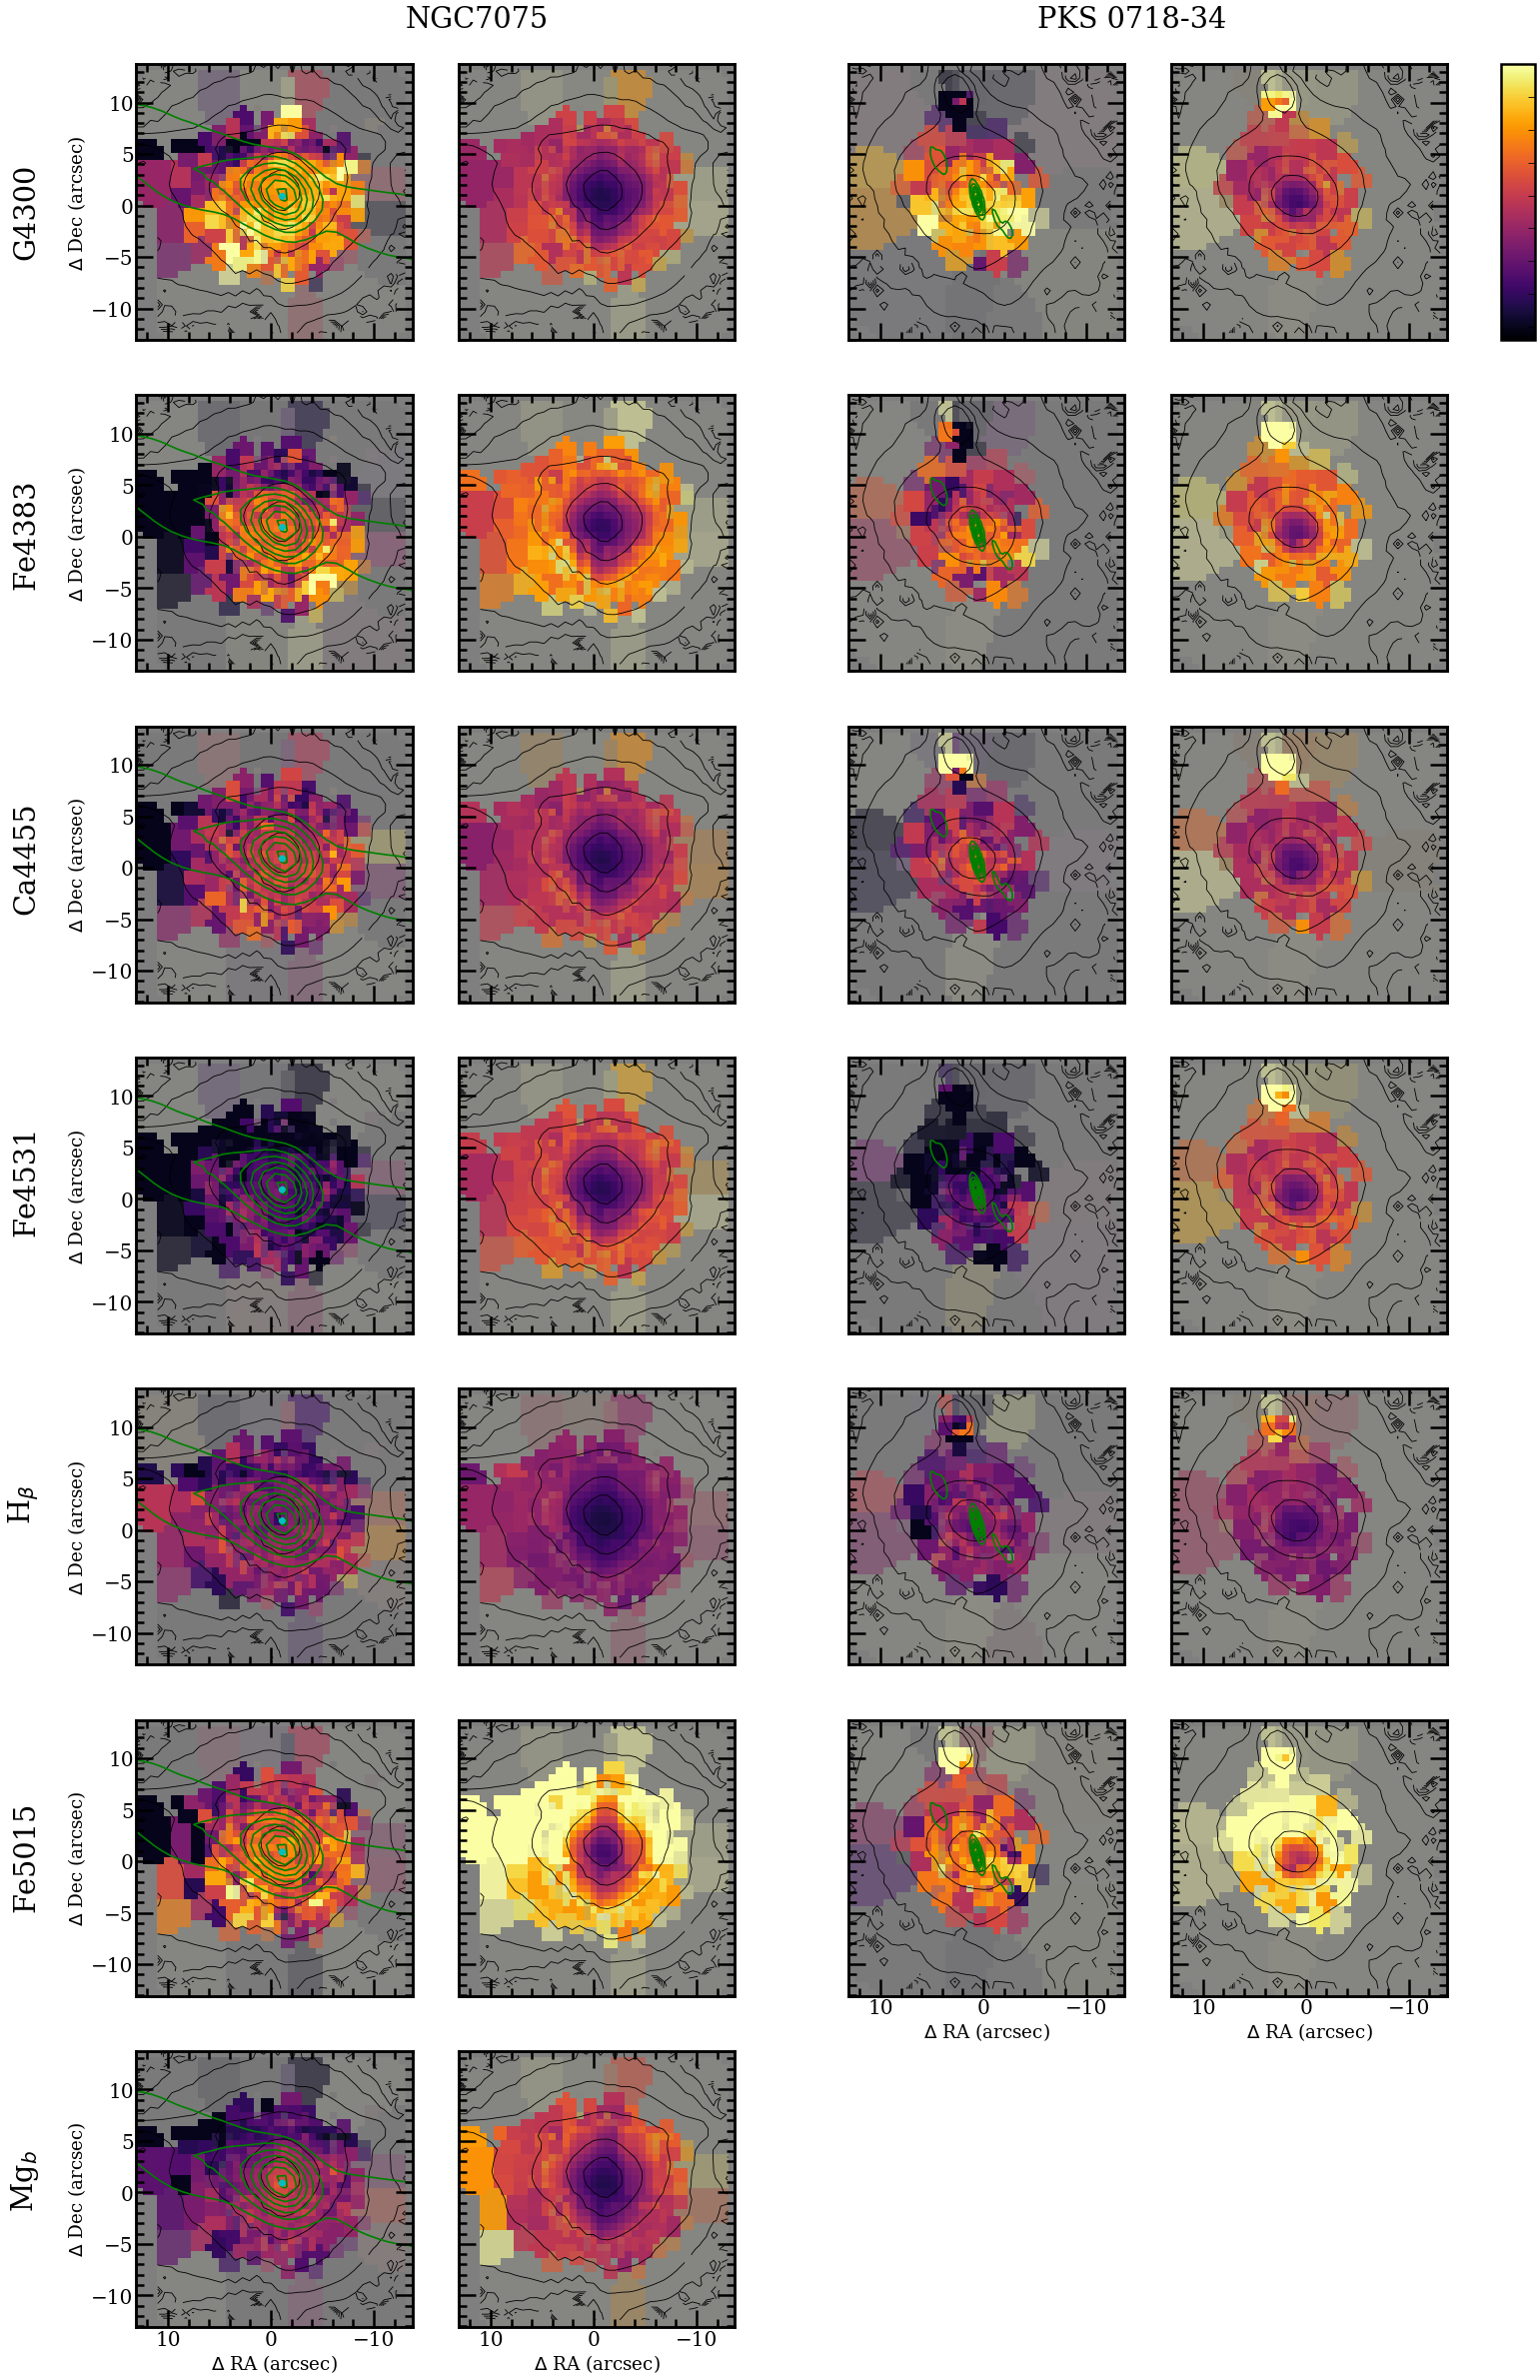
\includegraphics[height=0.94\textheight]{chapter4/vimos/abs5.png}
			\contcaption{\textit{Continued.}}% for NGC 7075 and PKS 718-34}
		\end{figure}

		\begin{figure}
			\centering
			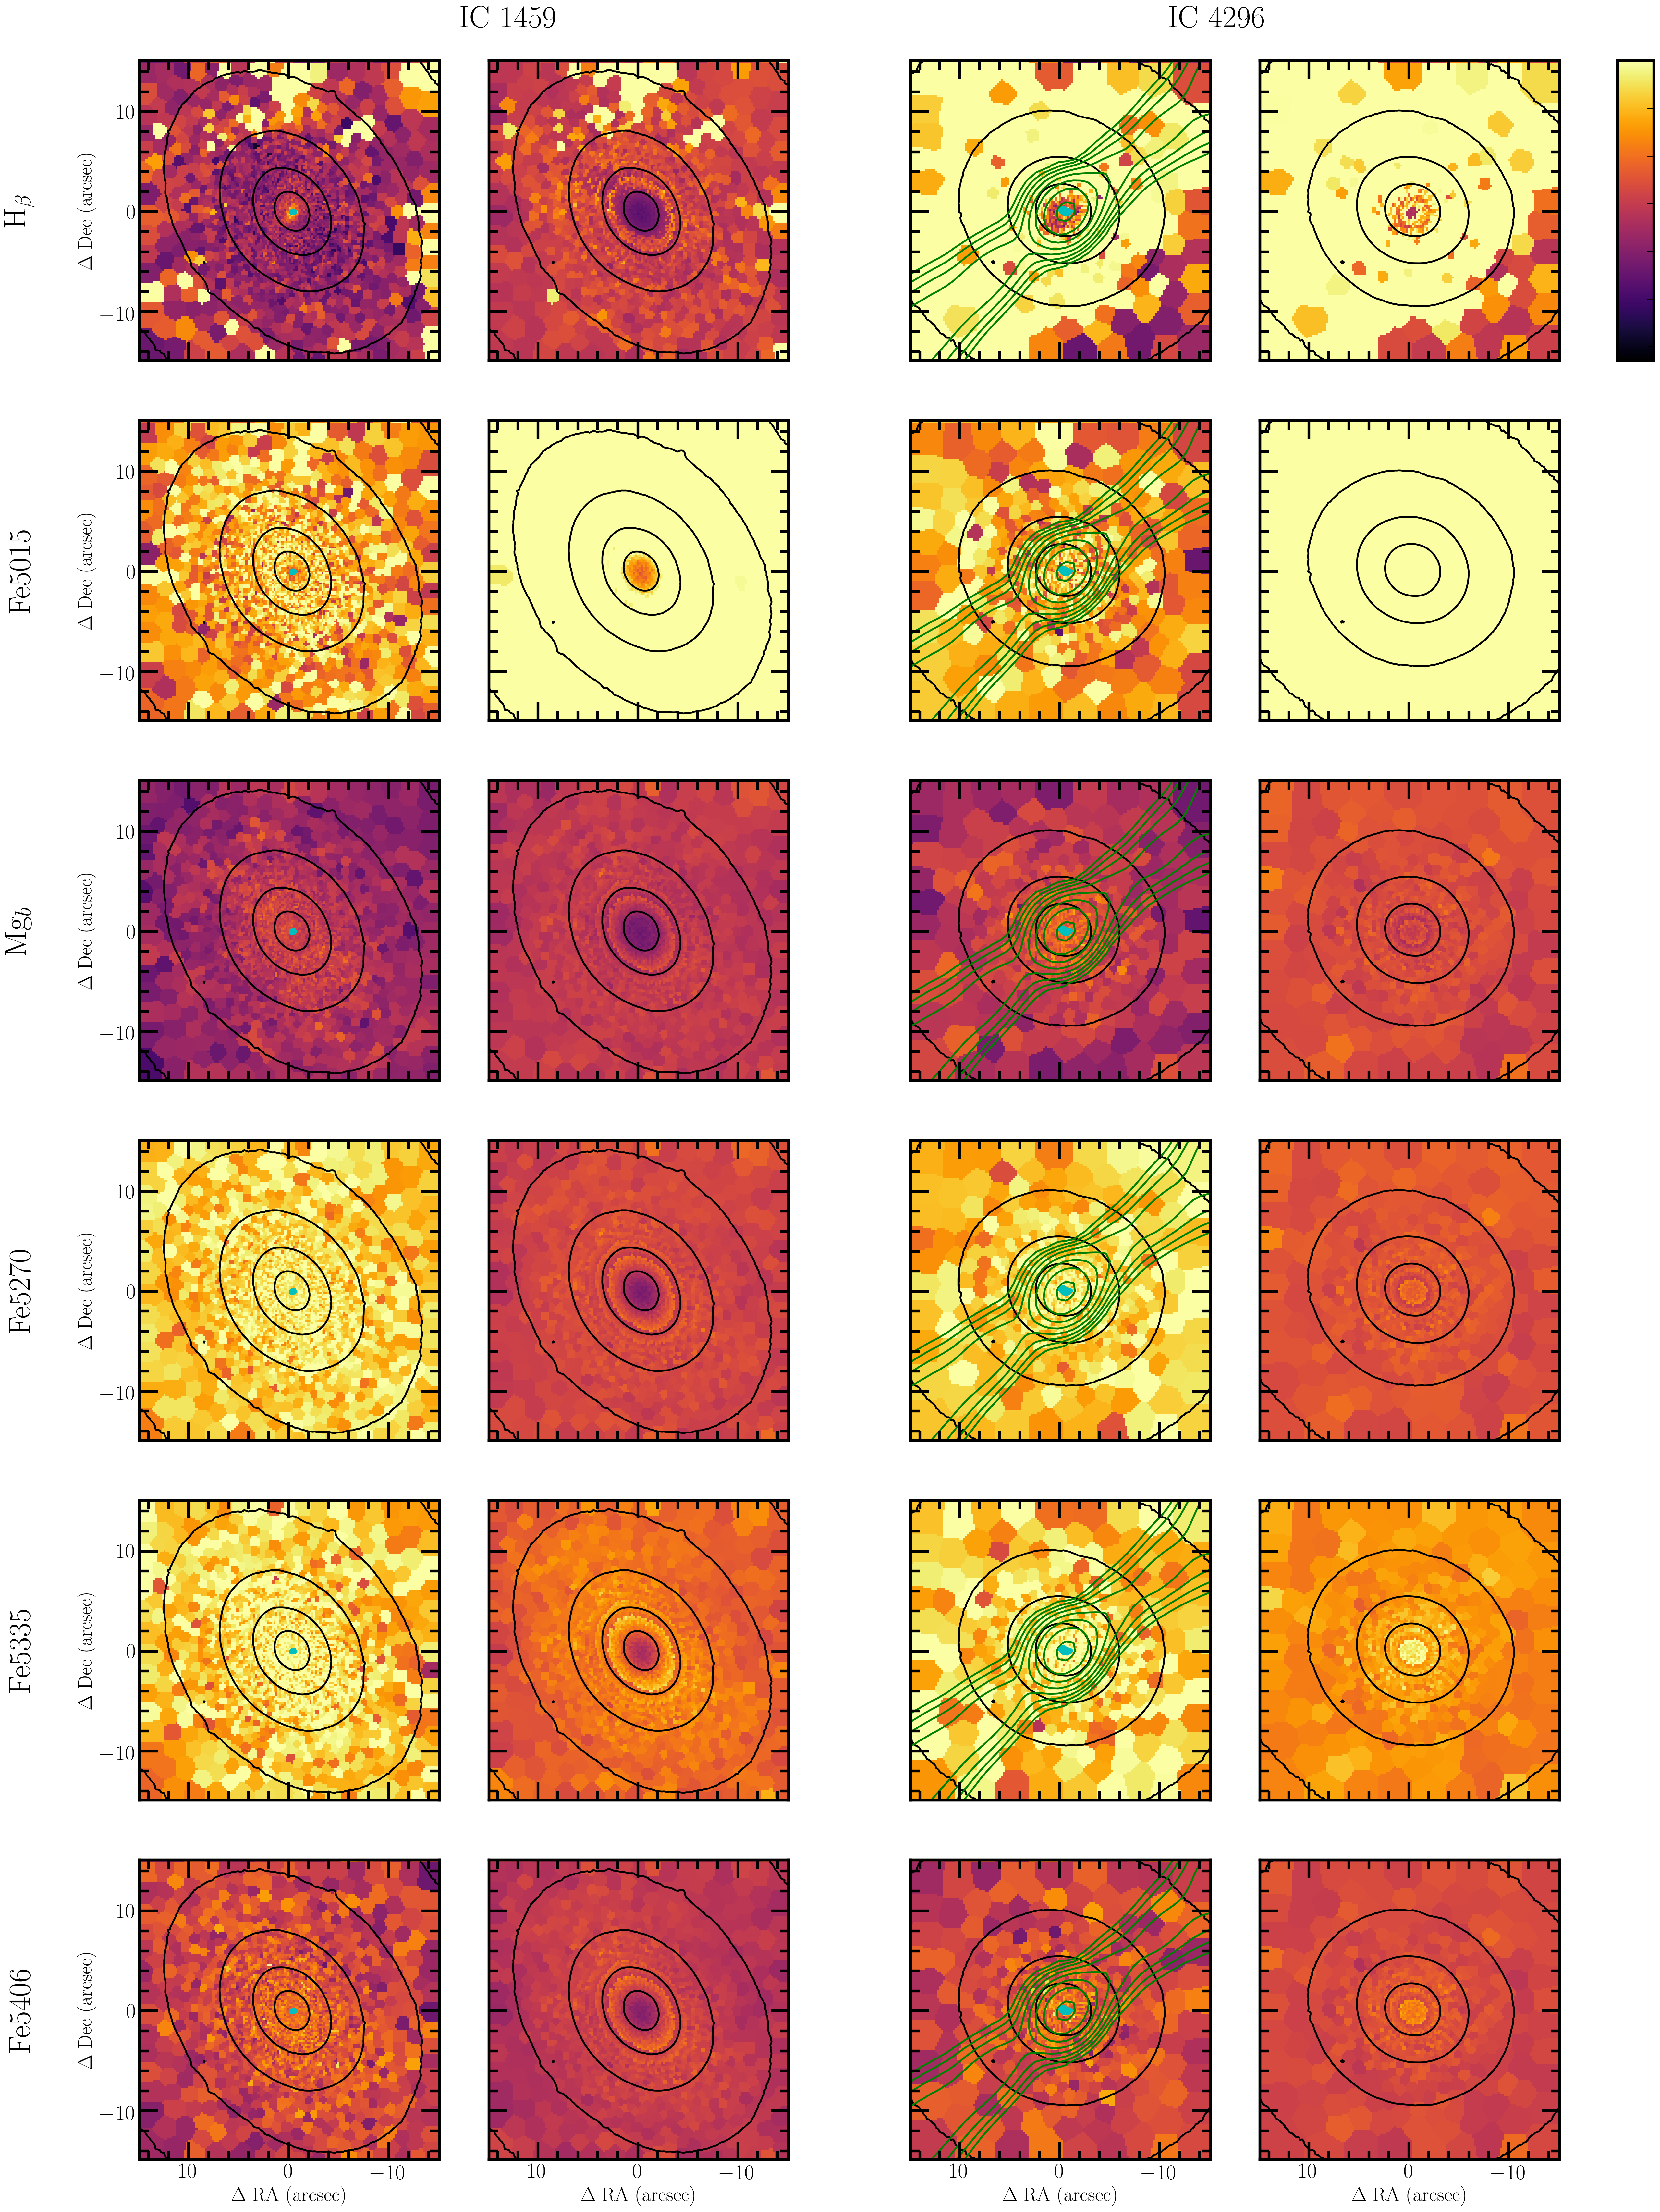
\includegraphics[height=0.81\textheight]{chapter4/muse/abs1.png}
			\caption[MUSE absorption line strength maps]{As Fig.\,\ref{fig:VIMOS_absorption} but for the MUSE absorption line strength maps. Limits on the colour scales are 0.5--3.5\,\AA\ for the H\,$\beta$, Fe5270, Fe 5335, Fe5406, Fe5709 and Fe5782 indices, 0--0.35\,mag for the TiO1 index, 0--0.1\,mag for the TiO2 index and 3--7\,\AA\ for all other indices. For the uncertainty maps the colour scale limits are 0--0.03\,mag for the TiO1 and TiO2 indices and 0--0.5\,\AA\ for all other indices.}
			\label{fig:MUSE_absorption}
		\end{figure}
		\begin{figure}
			\centering
			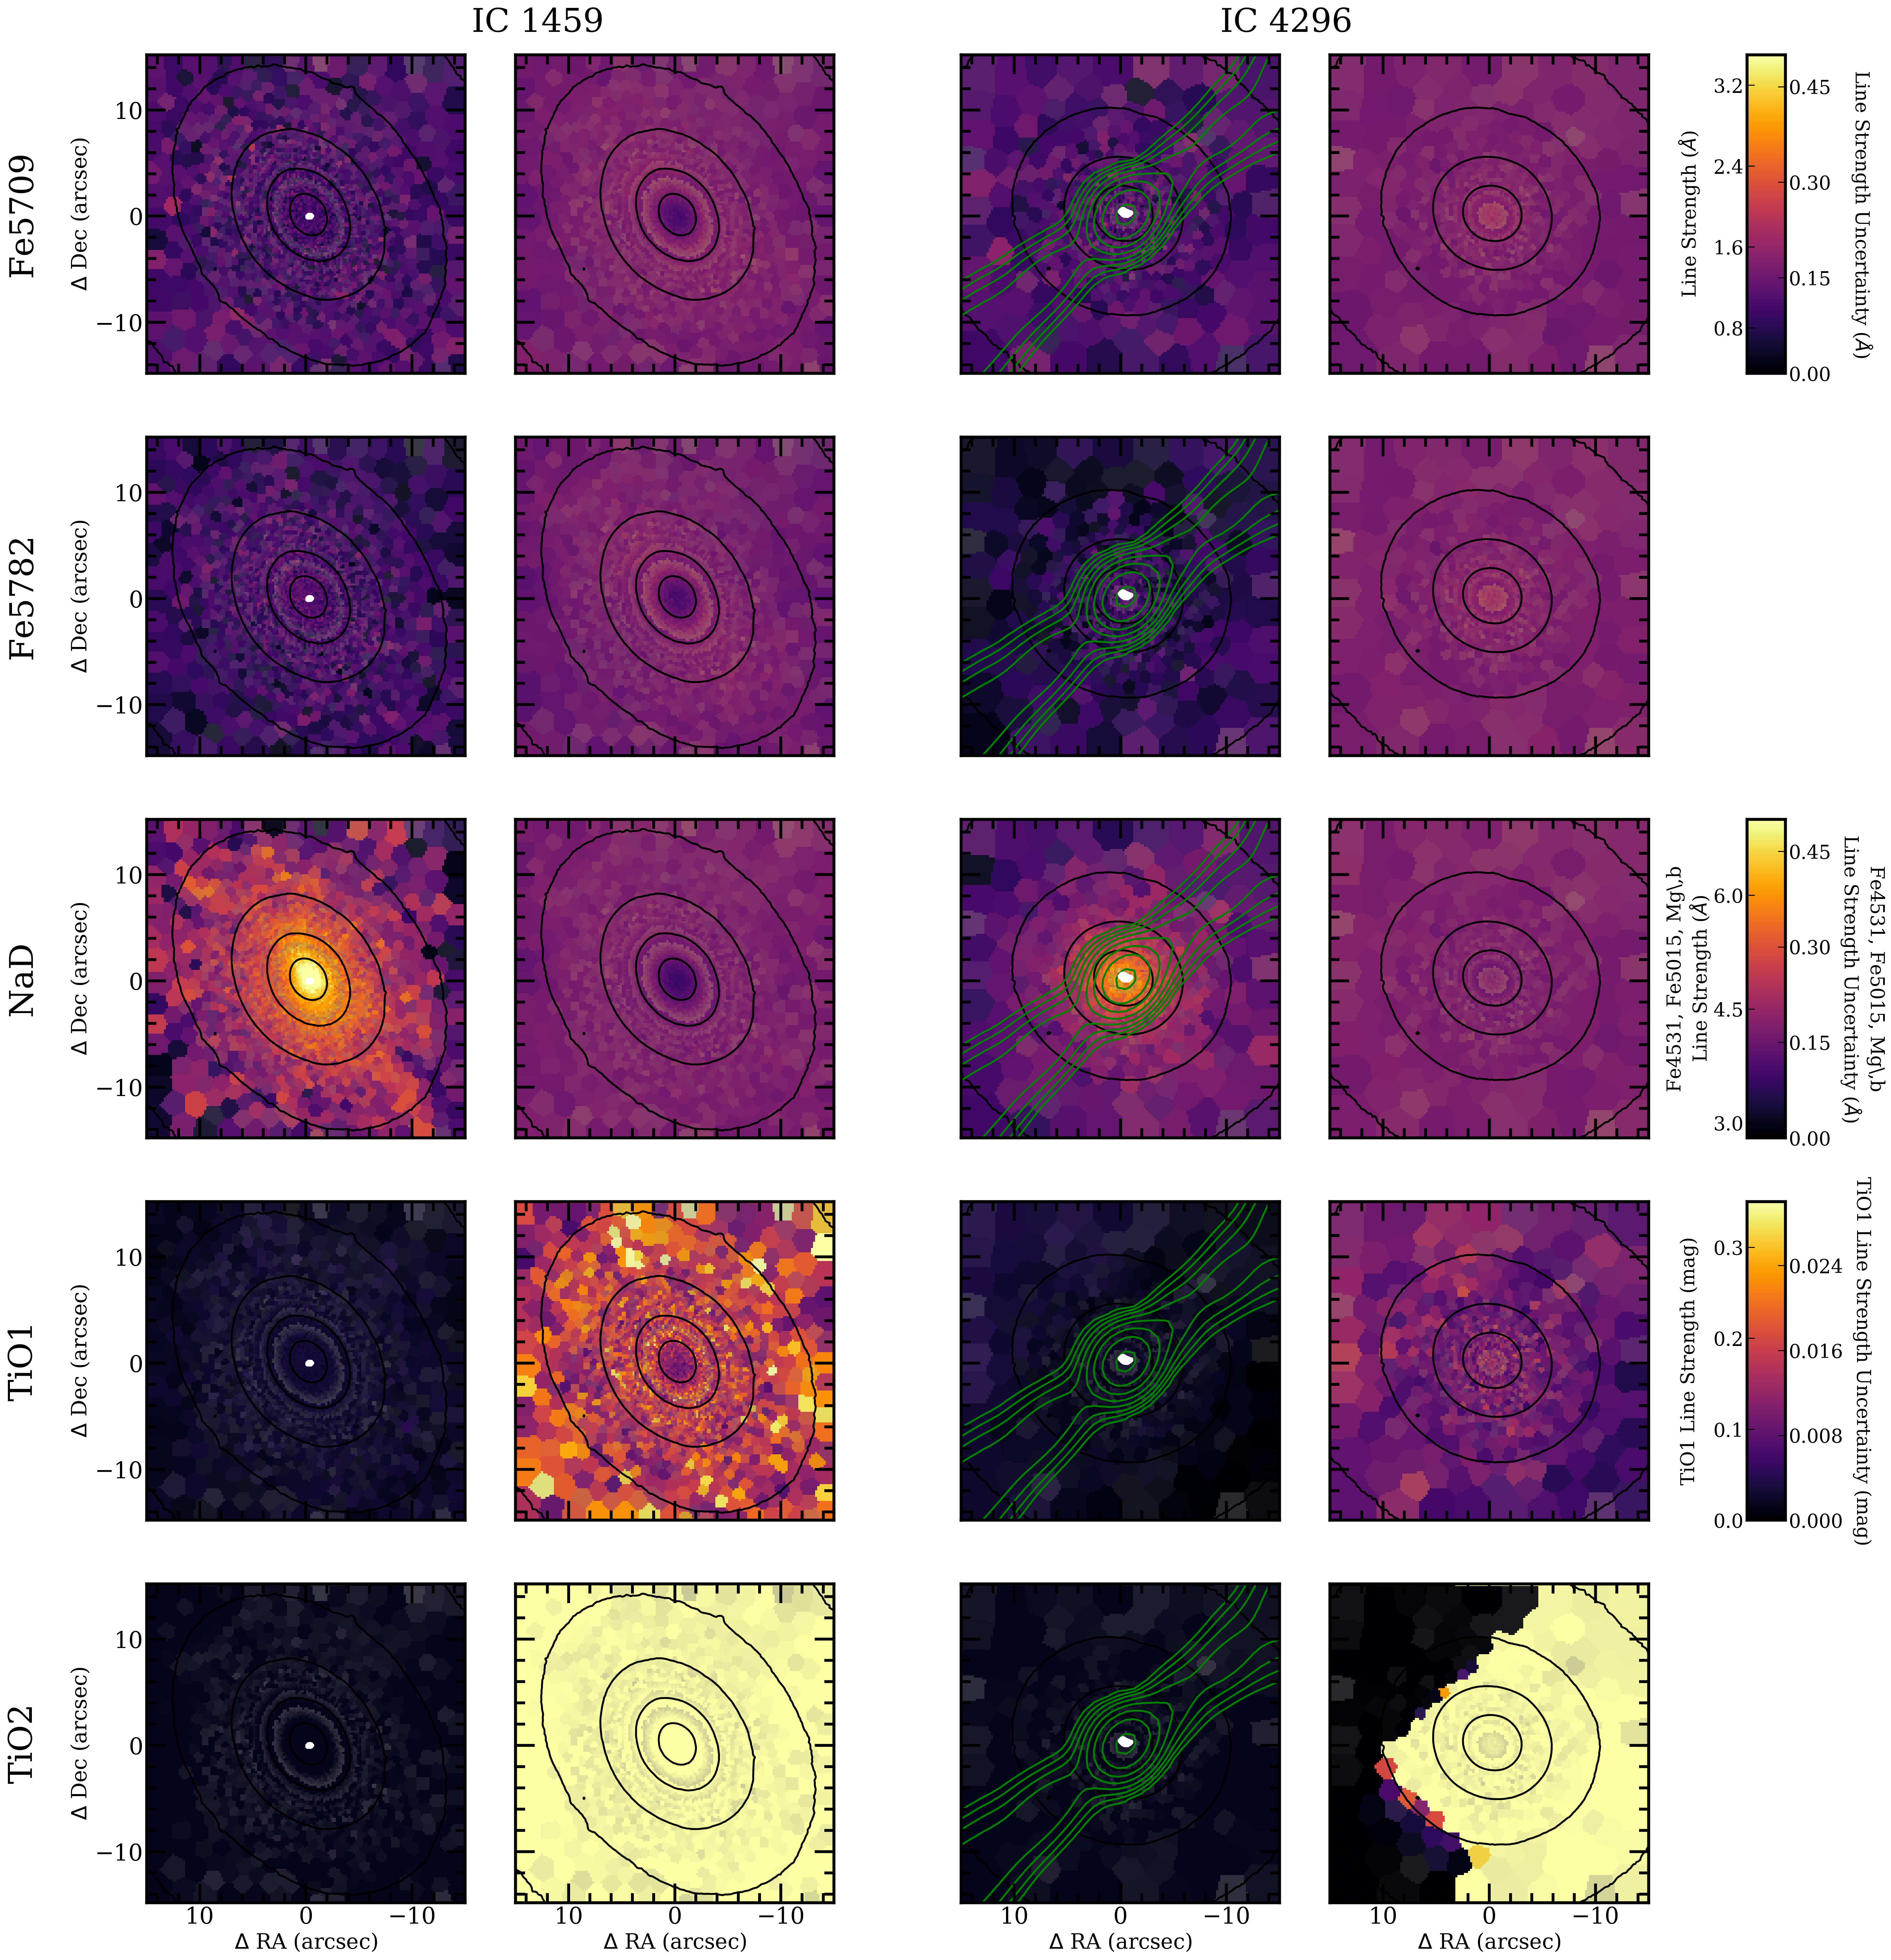
\includegraphics[height=0.67\textheight]{chapter4/muse/abs1b.png}
			\contcaption{\textit{Continued.}} %: From top to bottom: Fe5782, NaD, TiO1, TiO2. Plots are as in \ref{fig:VIMOS_stellar}. Limits on the colour scale are 0-9 \AA\ for the line strengths and 0-1 \AA\  for the uncertainties and 0-0.35 mag for TiO1 and TiO2 line strengths and 0-0.03 mag for the uncertainty in TiO1 and TiO2.}
		\end{figure}
		\begin{figure}
			\centering
			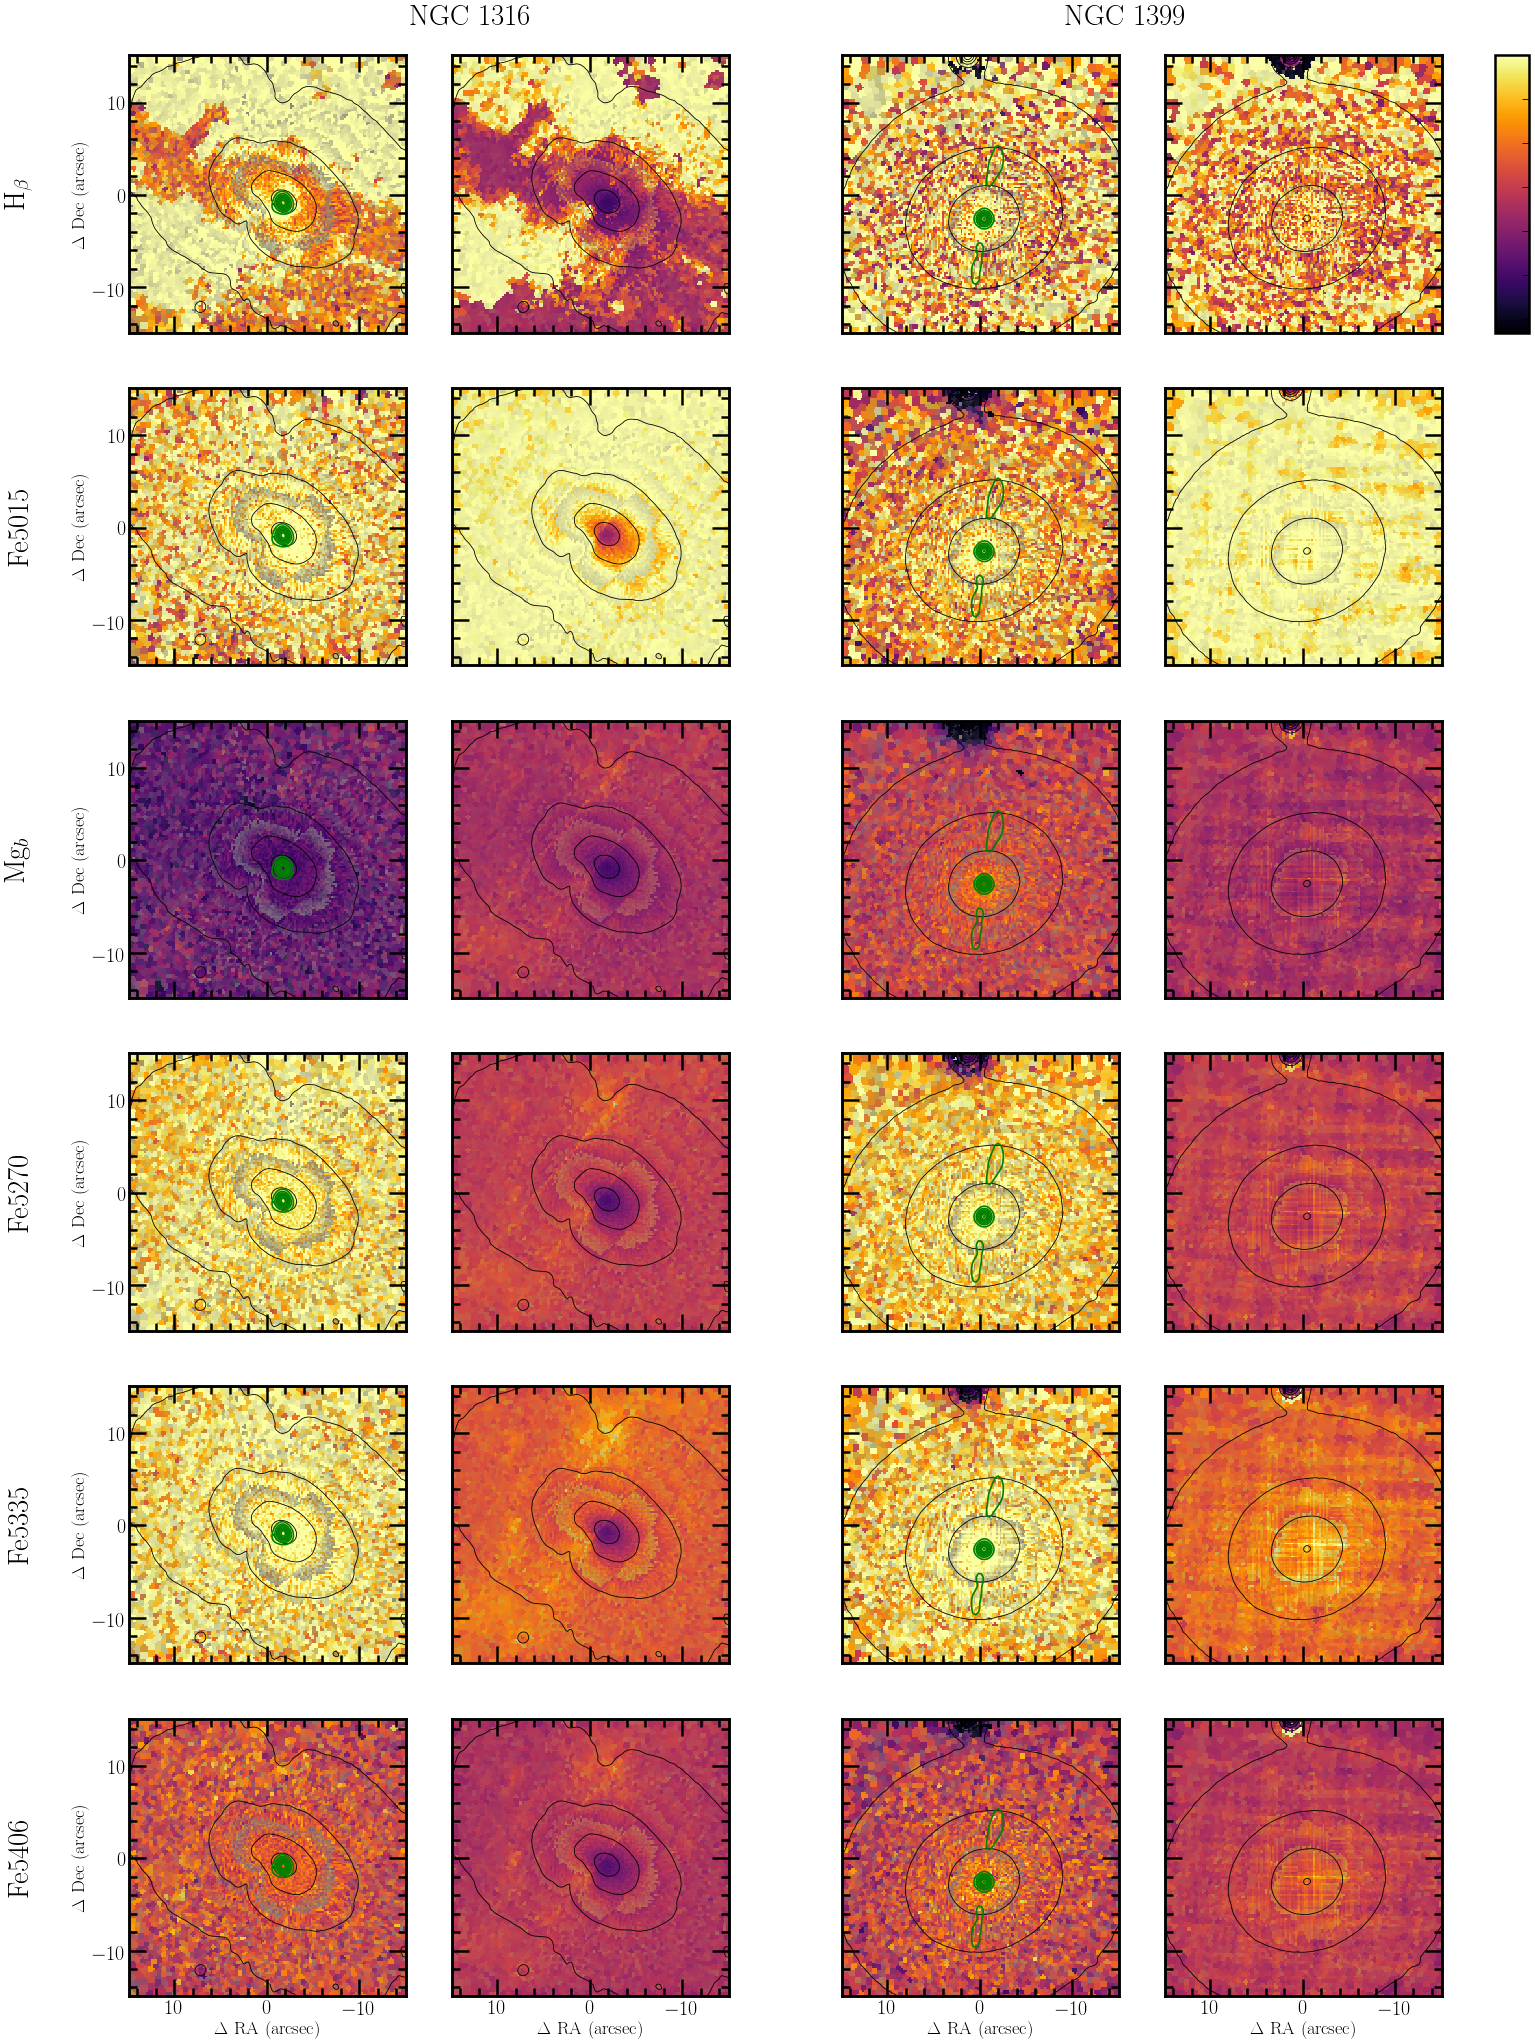
\includegraphics[height=0.81\textheight]{chapter4/muse/abs2.png}
			\contcaption{\textit{Continued.}}% for NGC1316 and NGC1399.}
		\end{figure}
		\begin{figure}
			\centering
			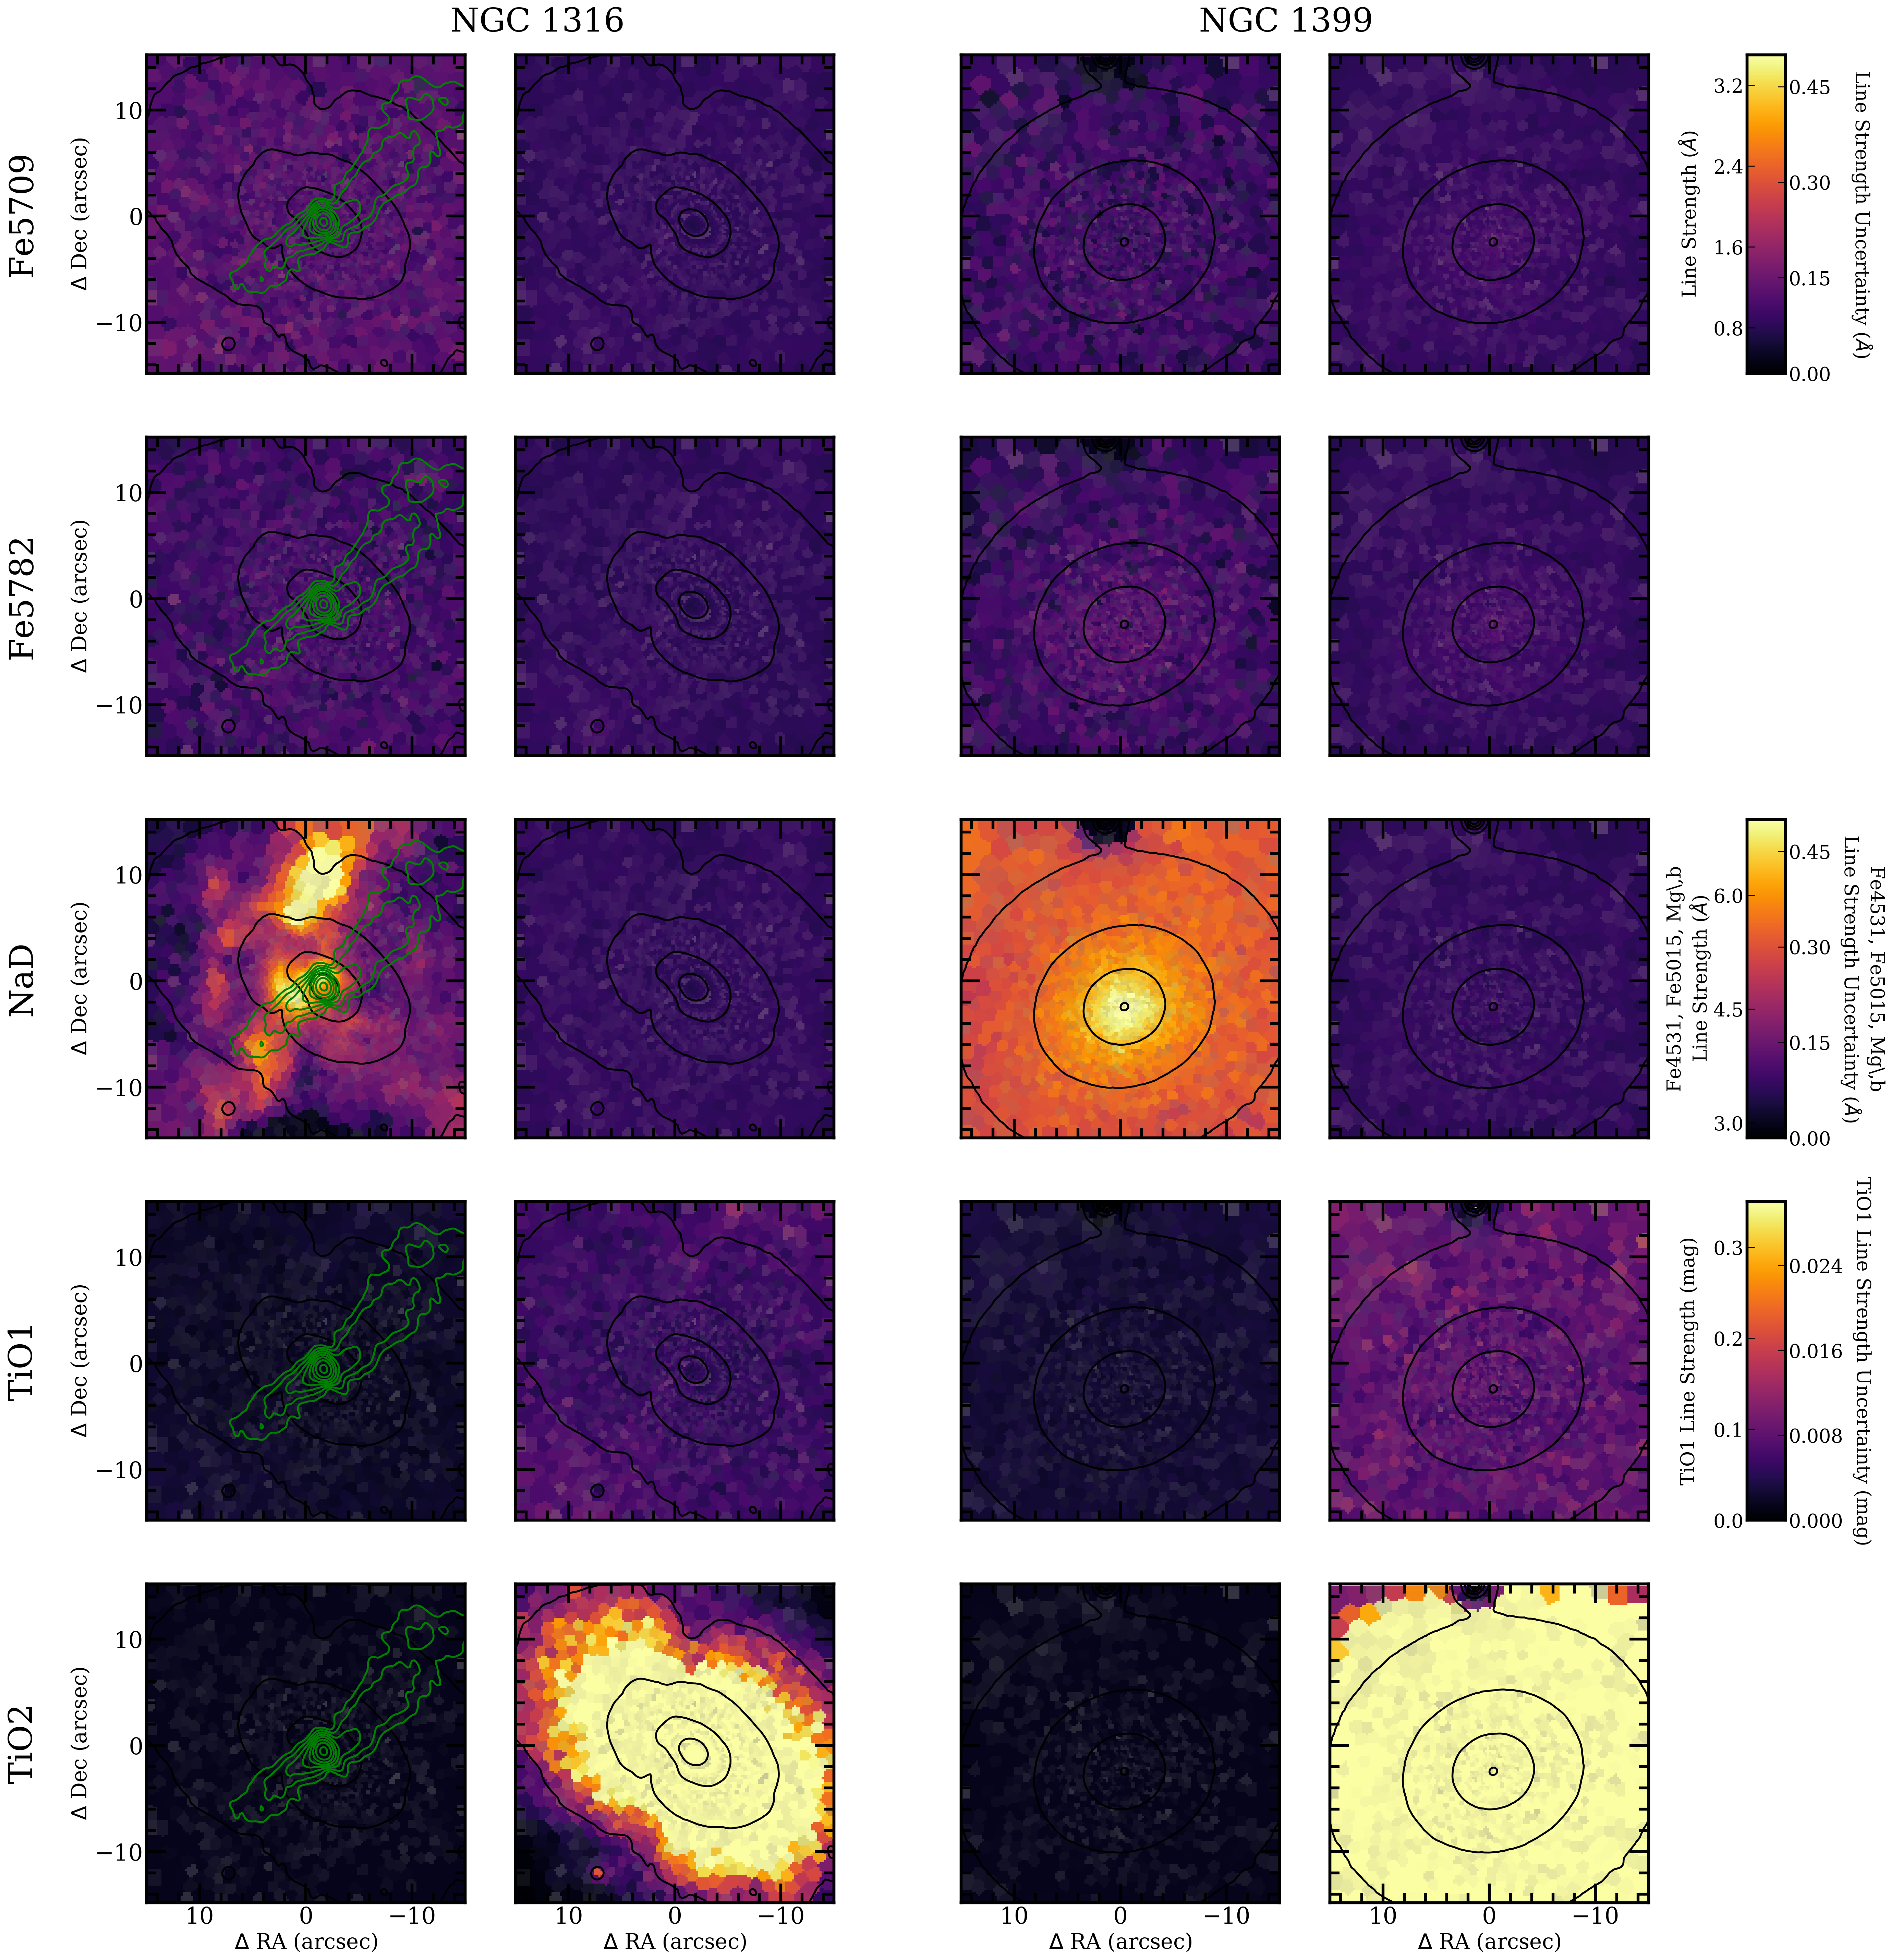
\includegraphics[height=0.67\textheight]{chapter4/muse/abs2b.png}
			\contcaption{\textit{Continued.}}% for NGC1316 and NGC1399.}
		\end{figure}

			We observe that most of our Southern sample show almost uniform, small H\,$\beta$ line strengths throughout a given galaxy, as well as slight central concentration in Fe, Ca4455 and Mg\,b index maps. NGC 612 is the exception to these trends, with large H\,$\beta$ line strengths, particularly along the dust lane and larger gradients in Fe and Ca4455 (see description in Appendix \ref{cha:Description}). The MUSE derived maps also show significant central concentration in the NaD index. The NaD feature is thought to be significantly deepened by absorption from the interstellar medium (ISM), if present \citep[e.g.][]{Phillips1993, Bergmann2009}, a concept consistent with the NaD line strength map of NGC 1316 where the strongest absorption is seen in the dust lane. Like NGC 612, NGC 1316 also has large H\,$\beta$ line strengths, again with the highest values along the dust lane. 

		\subsubsection{Mg\,--\,$\sigma$ relation}
			\label{subsubssec:Mgsigma}
			The definition of the Mg$_2$ absorption line index (blue continuum: 4895.125--4957.625\,\AA, index bandpass: 5154.125--5196.625\,\AA\ and red continuum: 5301.125--5366.125\,\AA) has overlapping bandpasses with the Mg\,b index, but includes the MgH molecular absorption line, and is hence considered a molecular index and is measured in units of magnitude. \citet{Bender1993} first noticed the unusually tight relationship between the global Mg$_2$ absorption line strength and logarithm of the central velocity dispersion, $\sigma_0$, in elliptical galaxies. They also noticed that residuals to the best-fitting line appeared to be intrinsic as they have a near Gaussian distribution about the median values, and do not seem to be correlated to any other galaxy property. 

			Since part of the red continuum band of the Mg$_2$ index is outside of the spectral range of VIMOS, but \citet{Ziegler1997} show there is a linear relationship between Mg\,b and Mg$_2$, with a gradient of 14.3--15.5\,mag\,\AA$^{-1}$\ depending on metallicity. We thus use Mg\,b as a proxy for Mg$_2$. 

			Using an aperture with a radius of 2\arcsec\ on each datacube, we measure $\sigma_0$ and Mg\,b at a spectral resolution of 8.4\,\AA\ full-width half-maximum (FWHM; see Table \ref{tab:globalMg} and points in Fig.\,\ref{fig:globalMg}). The best-fitting linear relationship (found using \textsc{lts\_linefit} by \citealt{Cappellari2013}) has a gradient of $2.3 \pm 0.5 \,\mathrm{\AA\,dex^{-1}}$ (solid black line in Fig.\,\ref{fig:globalMg}) with an intrinsic scatter of $0.13 \pm 0.10 \, \mathrm{\AA}$. Individual measurements for each galaxy are given in table \ref{tab:globalMg}.

			This is in very good agreement with the gradient found by \citet{Ziegler1997} for a sample of elliptical galaxies within Virgo and Coma using data from \citet{Dressler1987} of $2.5\,\mathrm{\AA\,dex^{-1}}$ (shown as the blue dotted line in Fig.\,\ref{fig:globalMg}), with an intrinsic scatter of 0.16\,\AA\ for galaxies with $\log \sigma_0 \geqslant 2.3$. 

			\begin{table}
				\centering
			\begin{threeparttable}
				\caption{The Mg\,b index and velocity dispersion within 2 arcsec from both MUSE and VIMOS datasets.}
				\label{tab:globalMg}
				\begin{tabular}{l c c c c}
					\hline
					\hline
					Galaxy 	& \multicolumn{2}{c}{Mg\,b} & \multicolumn{2}{c}{$\sigma_0$} \\
						& \multicolumn{2}{c}{\AA} & \multicolumn{2}{c}{km s$^{-1}$} \\
						& VIMOS & MUSE 	& VIMOS & MUSE \\
					\hline
					ESO 443-G024 & $4.42 \pm 0.03$ & -- & $220.8 \pm 0.8$ & -- \\
					IC 1459 	& $4.85\pm0.07$ & $4.66 \pm 0.012$ & $248.3\pm0.6$ & $311.5 \pm 1.6$ \\
					IC 1531 	& $4.01 \pm 0.04$ & -- & $149.6 \pm 1.1$ & -- \\
					IC 4296		& $4.66\pm0.03$ & $4.57 \pm 0.10$ &  $299.1\pm1.0$ & $338.5 \pm 2.1$ \\
					NGC 612 	& -- & -- & $228.0 \pm 3.0$ & -- \\
					NGC 1316 	& -- & $3.41 \pm 0.05$ & -- & $207.4 \pm 1.3$ \\
					NGC 1399 	& $5.39\pm0.11$ & $4.90 \pm 0.13$ & $282.2\pm0.6$ & $303.0 \pm 2.9$ \\
					NGC 3100 	& $4.37 \pm 0.04$ & -- & $134.6 \pm 0.9$ & -- \\
					NGC 3557 	& $4.26 \pm 0.04$ & -- & $232.9 \pm 0.4$ & -- \\
					NGC 7075 	& $4.43 \pm 0.06$ & -- & $194.5 \pm 1.4$ & -- \\
					PKS 718-34  & -- 		      & -- & $217.0 \pm 1.6$ & -- \\
					\hline
					\hline
				\end{tabular}
				\begin{tablenotes}
				\footnotesize
				\note Part of the red continuum bandpass of the Mg\,b index in NGC 612 and PKS 718-34 is redshifted outside of the wavelength range of VIMOS.
				\end{tablenotes}
			\end{threeparttable}
			\end{table}


			\begin{figure}
				\centering
				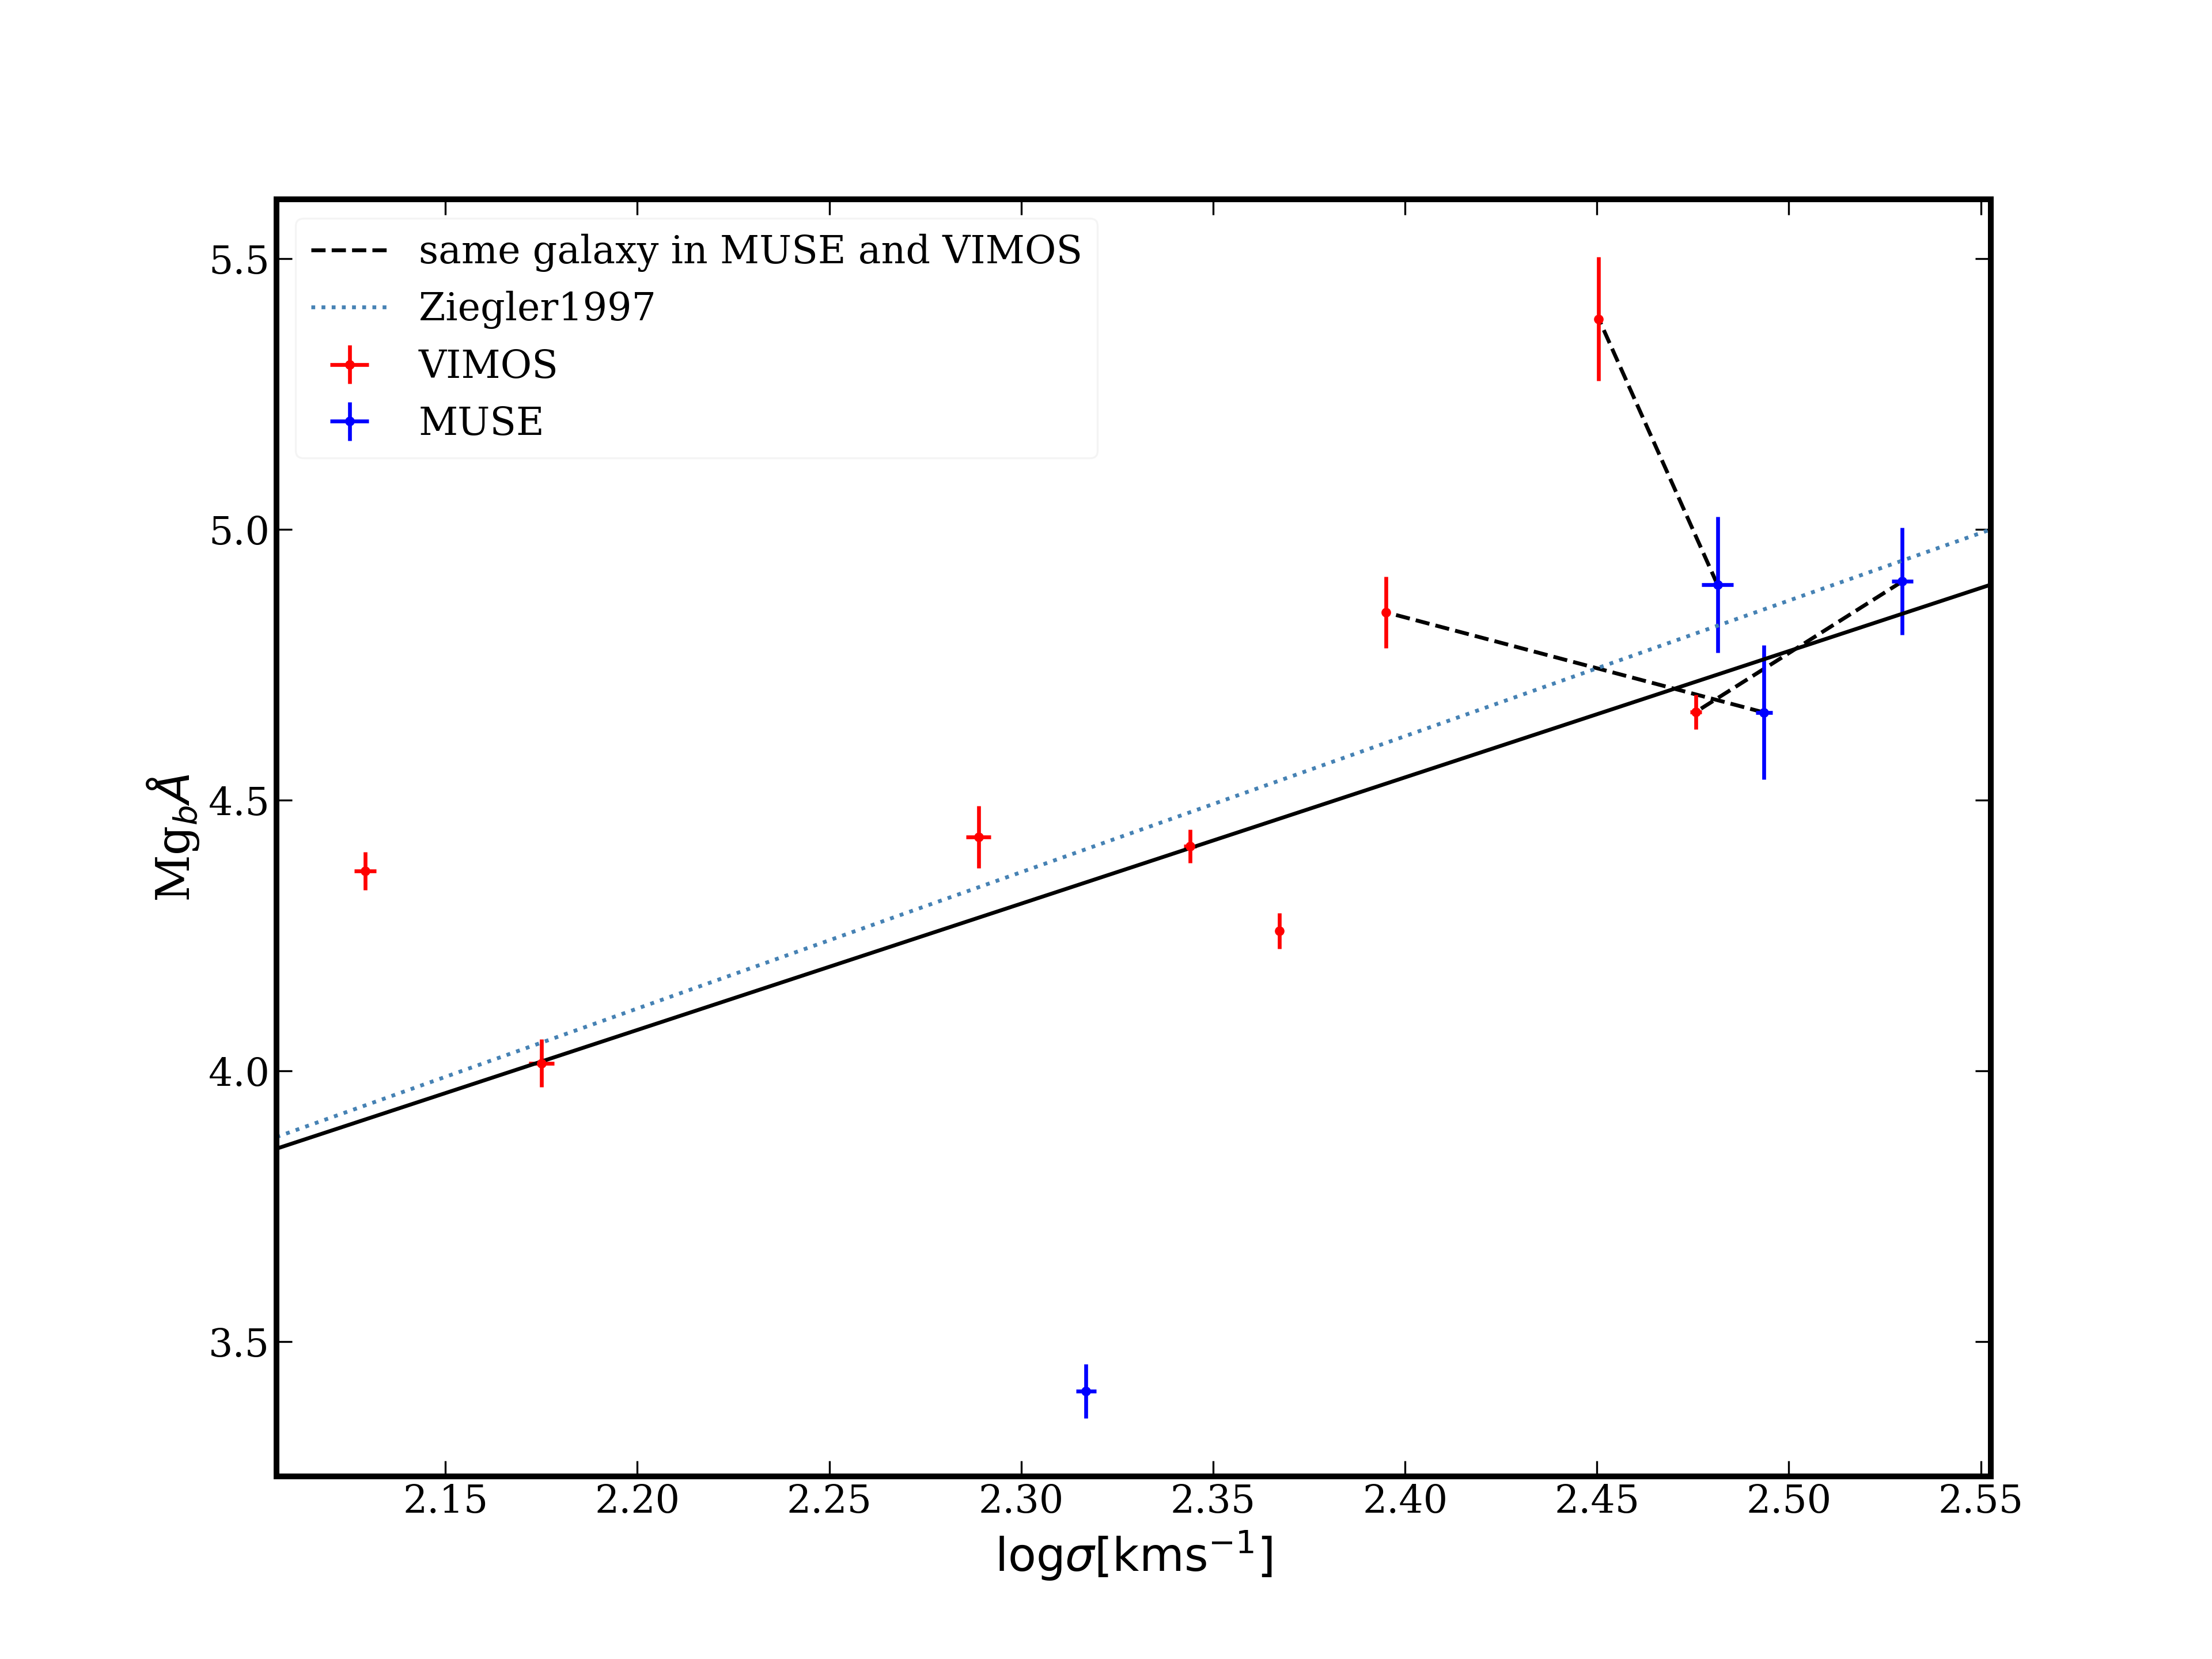
\includegraphics[width=.8\textwidth]{chapter4/Mg_sigma.png}
				\caption[Global Mg\,b\,--\,$\sigma$]{The Mg\,b\,--\,velocity dispersion relation using a 2\arcsec aperture. We find a similar gradient to our best-fitting (solid) as that found by \citet[; dotted line]{Ziegler1997}.}
				\label{fig:globalMg}
			\end{figure}

			\citet{Mehlert2003} shows the existence of the internal Mg\,--\,$\mathrm{\sigma}$ relation, but also suggests that it has a different origin to that of the global relation. They found that alpha-enhancement correlates with velocity dispersion and drives about 30\% of the global Mg\,--\,$\sigma$ relation, with metallicity variations providing the remaining 70\%. Alpha-enhancement usually has no radial gradient (while velocity dispersion is highly dependent on radius) suggesting that alpha-enhancement has no role in the internal Mg\,--\,$\sigma$ relation and it is entirely due to the metallicity radial gradient. We therefore have not shown the internal Mg\,--\,$\sigma$ relationships. Instead we investigate radial gradients of the most-likely simple stellar populations (SSPs) in Section \ref{subsubsec:popGrad}.


		\subsubsection{Comparison to the Literature}
			\label{subsubsec:Lit}

			A comparison to the literature is difficult because of the inhomogeneous corrections applied by different authors. There are no standardized methods for accounting for emission lines from the ISM and/or stellar velocity dispersion. For example, some authors only correct for H\,$\beta$ emission, despite [\ion{O}{iii}] often being the strongest emission line in ETGs. This will effect the reliability of the Fe5015 index, since the [\ion{O}{iii}] doublet falls within its bandpasses. [\ion{N}{i}] emission will affect the Mg\,b index in the same way, although obviously not as strongly.

			Some indices are extremely sensitive to the stellar velocity dispersion correction. For example, due to the steepness of the pseudo-continuum in the G4300 index, a change of $30 \, \mathrm{km\,s^{-1}}$ in the velocity dispersion can effect the dispersion corrected index value by as much as 2\,\AA.

			When comparing to a particular paper we correct for the same effects described in the paper, but using our methods, as described in Section \ref{subsubsec:Absorption}. We use a resolution of 8.4\,\AA\ (FWHM) in order to use the transformation function provided by \citet{Vazdekis2010} to convert from Lick calibrated measurements to the Line Index System (LIS; see Section \ref{subsubsec:Absorption}). 

			Table \ref{tab:litAbsorption} summarises our comparisons to the literature. For the comparison to \citet{Vazdekis2010}, we analysed the SAURON dataset\footnote{\url{http://www.strw.leidenuniv.nl/sauron/}} \citep{Emsellem2004} using the same analysis pipeline as for our Southern Sample. 


			\begin{table}
				\centering
			\begin{threeparttable}
				\caption{Comparisons of measured absorption line indices to the literature.}
				\label{tab:litAbsorption}
				\begin{tabular*}{0.8\textwidth}{@{\extracolsep{\fill}}l r r r}
					\hline
					\hline
					Index 		& \multicolumn{1}{c}{N$_\mathrm{gals}$} & \multicolumn{1}{c}{Offset} & \multicolumn{1}{c}{Dispersion} \\
								& 		&\multicolumn{1}{c}{\AA}& \multicolumn{1}{c}{\AA} \\
					\hline
					\multicolumn{4}{c}{\citet{Vazdekis2010} (SAURON)} \\
					\hline
					H\,$\beta$ 	& 46		& -0.02\leavevmode\phantom{0}& 0.25\leavevmode\phantom{0}	\\
					Fe5015		& 46		& 0.66\leavevmode\phantom{0}& 0.34\leavevmode\phantom{0}	\\
					Mg\,b 		& 46		& 0.06\leavevmode\phantom{0}& 0.33\leavevmode\phantom{0}	\\
					\hline
					\multicolumn{4}{c}{\citet{Rampazzo2005} (VIMOS)} \\
					\hline
					G4300 		& 3 		& 2.29\leavevmode\phantom{0}& 0.11\leavevmode\phantom{0}	\\
					Fe4383 		& 3 		& 0.39\leavevmode\phantom{0}& 0.23\leavevmode\phantom{0}	\\
					Ca4455 		& 3 		& -0.19\leavevmode\phantom{0}& 0.09\leavevmode\phantom{0}	\\
					Fe4531 		& 3 		& 0.16\leavevmode\phantom{0}& 0.26\leavevmode\phantom{0}	\\
					H\,$\beta$ 	& 3 		& 0.17\leavevmode\phantom{0}& 0.12\leavevmode\phantom{0}	\\
					Fe5015 		& 3 		& -0.73\leavevmode\phantom{0}& 0.48\leavevmode\phantom{0}	\\
					Mg\,b 		& 3 		& -0.43\leavevmode\phantom{0}& 0.17\leavevmode\phantom{0}	\\
					\hline
					\multicolumn{4}{c}{\citet{Rampazzo2005} (MUSE)} \\
					\hline
					H\,$\beta$ 	& 2 		& -0.28\leavevmode\phantom{0}& 0.17\leavevmode\phantom{0}	\\ 
					Fe5015 		& 2 		& 0.87\leavevmode\phantom{0}& 0.34\leavevmode\phantom{0}	\\ 
					Mg\,b 		& 2 		& 0.31\leavevmode\phantom{0}& 0.14\leavevmode\phantom{0}	\\
					Fe5270 		& 2 		& -0.11\leavevmode\phantom{0}& 0.15\leavevmode\phantom{0}	\\
					Fe5335 		& 2 		& 0.08\leavevmode\phantom{0}& 0.15\leavevmode\phantom{0}	\\
					Fe5406 		& 2 		& 0.16\leavevmode\phantom{0}& 0.07\leavevmode\phantom{0}	\\
					Fe5709 		& 2 		& 0.11\leavevmode\phantom{0}& 0.10\leavevmode\phantom{0}	\\
					Fe5782 		& 2 		& -0.03\leavevmode\phantom{0}& 0.11\leavevmode\phantom{0}	\\
					NaD 		& 2 		& 0.90\leavevmode\phantom{0}& 0.41\leavevmode\phantom{0}	\\
					TiO1 (mag)	& 2 		& -0.004	& 0.003	\\
					TiO2 (mag)	& 2 		& -0.011	& 0.007	\\
					\hline
					\multicolumn{4}{c}{\citet{Ogando2008} (VIMOS)} \\
					\hline
					H\,$\beta$ 	& 6 		& 0.07\leavevmode\phantom{0}& 0.60\leavevmode\phantom{0}	\\
					Fe5015 		& 6 		& -0.09\leavevmode\phantom{0}& 0.15\leavevmode\phantom{0}	\\
					Mg\,b 		& 6 		& -0.70\leavevmode\phantom{0}& 0.08\leavevmode\phantom{0}	\\
					\hline
					\multicolumn{4}{c}{\citet{Ogando2008} (MUSE)} \\
					\hline
					H\,$\beta$ 	& 3 		& -0.04\leavevmode\phantom{0}& 0.23\leavevmode\phantom{0}	\\ 
					Fe5015 		& 3 		& -0.16\leavevmode\phantom{0}& 0.33\leavevmode\phantom{0}	\\ 
					Mg\,b 		& 3 		& -1.10\leavevmode\phantom{0}& 0.26\leavevmode\phantom{0}	\\
					Fe5270 		& 3 		& -0.66\leavevmode\phantom{0}& 0.16\leavevmode\phantom{0}	\\
					Fe5335 		& 3 		& -0.66\leavevmode\phantom{0}& 0.11\leavevmode\phantom{0}	\\
					Fe5406 		& 3 		& -0.51\leavevmode\phantom{0}& 0.06\leavevmode\phantom{0}	\\
					Fe5709 		& 3 		& -0.22\leavevmode\phantom{0}& 0.08\leavevmode\phantom{0}	\\
					NaD 		& 3 		& -1.57\leavevmode\phantom{0}& 0.16\leavevmode\phantom{0}	\\
					\hline
					\hline
				\end{tabular*}
				\begin{tablenotes}
				\footnotesize
				\note Comparisons to \citet{Rampazzo2005} are sampled at 7 radial apertures for each galaxy: 1.5, 2.5 and 10.0 arcsec and R$_e$/10, R$_e$/8, R$_e$/4 and R$_e$/2. 
				\item Col.\,1: Index. Col.\,2: Number of galaxies in comparison. Col.\,3: Offset equals the mean of the measurements from the literature subtract our measurements. Col.\,4: Dispersion equals the standard deviation of the measurements from the literature subtract our measurements.
				\end{tablenotes}
			\end{threeparttable}
			\end{table}

			We find a very large offset for the G4300 index with respect to the results of \citet{Rampazzo2005}. As noted above, this index is extremely sensitive to the stellar velocity dispersion correction and we measure an average difference in the stellar velocity dispersion to that measured by \citet{Rampazzo2005} of $21\,\mathrm{km\,s^{-1}}$. This may be enough to account for the difference in the measurements.

			We also observe that the offset in the Fe5015 index is also quite large in comparisons with \citet{Rampazzo2005} and \citet{Vazdekis2010}. In the case of the comparison with \citet{Rampazzo2005} we suggest that the difference is due to differences in method for accounting for the [\ion{O}{iii}] emission lines, however the origin of the offset is less clear in case of the comparison with \citet{Vazdekis2010}. 

			Other than G4300 and Fe5015, the comparisons show fairly consistent agreement with literature measurements although the dispersion of the comparisons are fairly large. We suggest that the translation between Lick and LIS systems may be the source of this spread.


		\subsubsection{Robustness of Absorption Line Strength Results}
			\label{subsubsec:RobustAbs}
			As well as comparison to the literature, we also compare the Mg\,b radial profiles between the VIMOS and MUSE datasets (see Fig.\,\ref{fig:compare_mgb}) for the 3 galaxies for which we have both observations. As in Fig.\,\ref{fig:compare_sigprofile}, the degradation of VIMOS measurements at large radii from the galaxy's centre is immediately apparent. It is also immediately clear, that at lower radii the lines strengths from the VIMOS datasets are much more tightly constrained than the MUSE line strengths. This is particularly evident in IC 1459 where in the MUSE dataset, the Mg\,b line strengths has a double peak which occur in the outer regions of the KDC, however this feature is not seen in the VIMOS measurements. 

			\begin{figure}
				\centering
				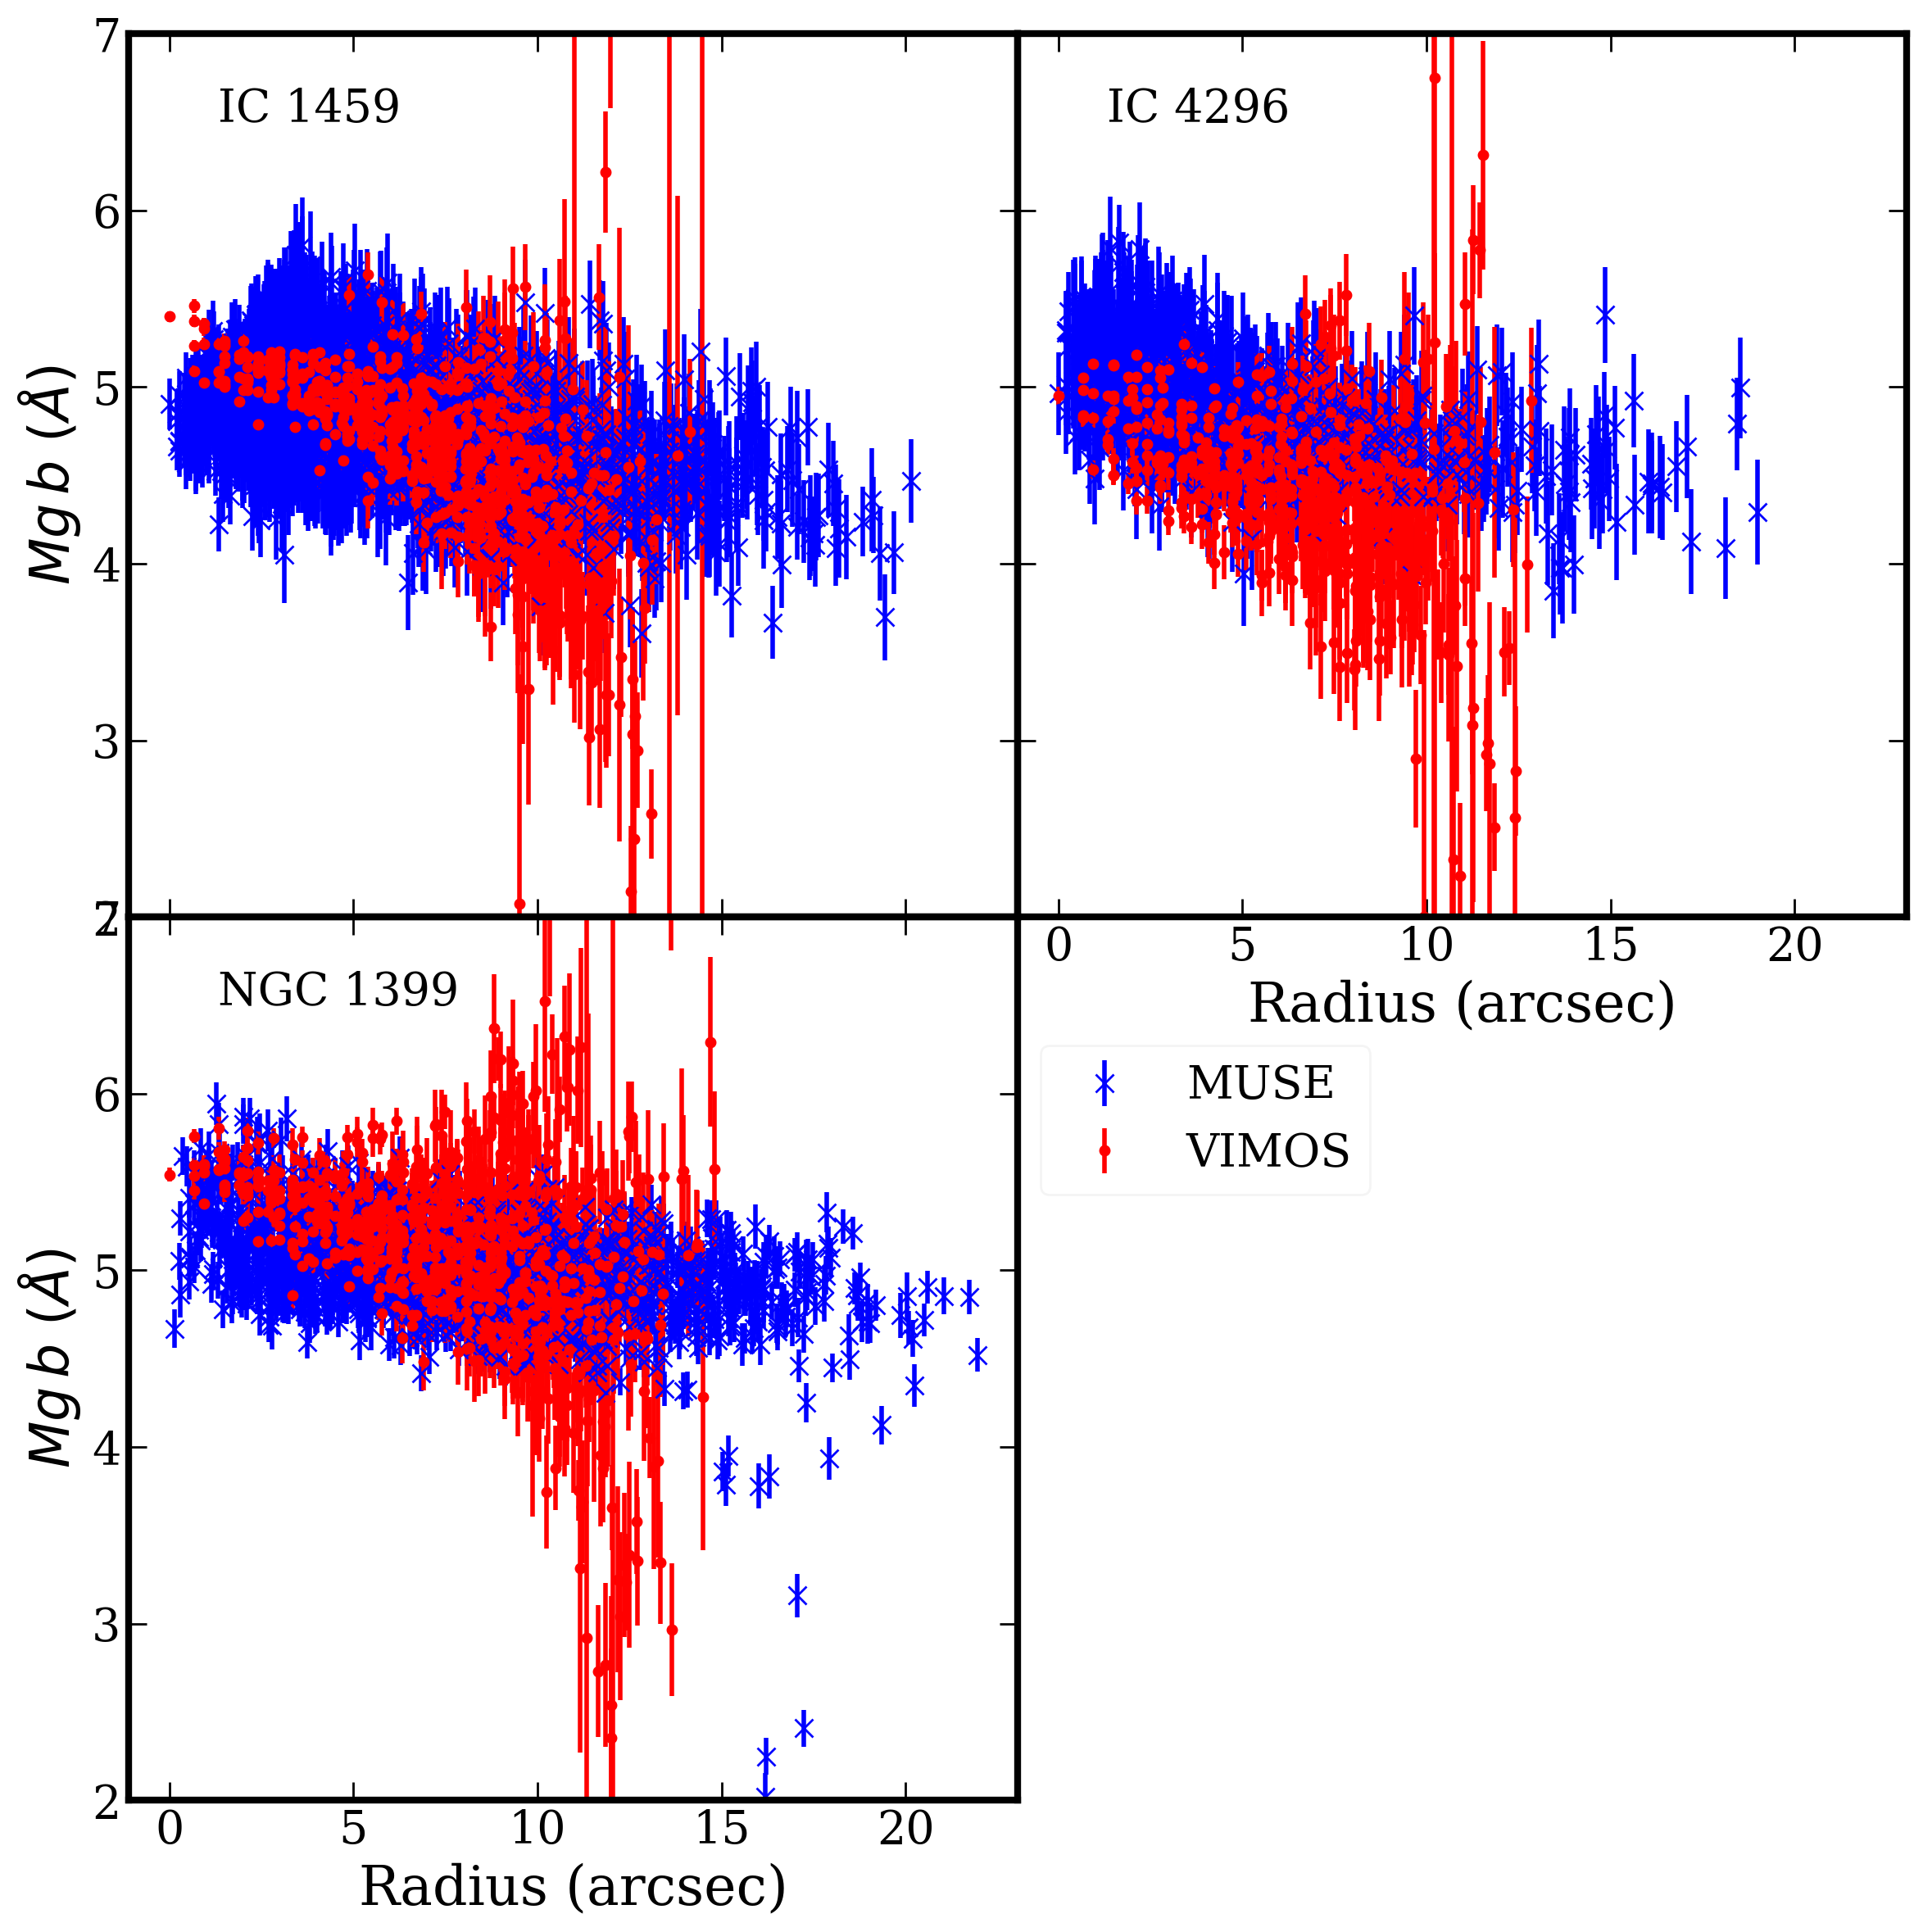
\includegraphics[width=.9\textwidth]{chapter4/compare_Mgb.png}
				\caption[Comparison between Mg\,b radial profiles from VIMOS and MUSE datacubes]{A comparison of the Mg\,b absorption line strengths for VIMOS (red) and MUSE (blue) datasets.}
				\label{fig:compare_mgbprofile}
			\end{figure}

			Overall the two datasets appear to be consistent with each other even in the cases of IC 4296 and NGC 1399 which both have large artifacts from the VIMOS instrument (see Section \ref{subsec:VIMOSartefacts}). 


	\subsection{Most-likely Stellar Population Models}
		\label{subsec:ssp}
		We have assumed that a given spectrum from our Southern sample can be well approximated by a SSP. We use the method described in Section \ref{subsubsec:StellarPop} to produce maps of the most-likely SSP characteristics: age ($t$), metallicity ($Z/H$) and alpha-element enhancement ($\alpha$/Fe) from the absorption line strength maps. 

		Figs.\,\ref{fig:VIMOS_pop} and \ref{fig:MUSE_pop} show the resolved most-likely stellar populations for our Southern sample. In general they show old, metal rich and alpha enhanced SSPs; qualities which ETGs are well known for. The exceptions are NGC 612 and NGC 1316. Both galaxies are described in more detail in Appendix \ref{cha:Description}, but NGC 1316 shows a very young stellar population (our fit of $t \approx 2$\,Gyr agrees with that of \citealt{Kuntschner2000}, but is conflicting with the older and less metal rich stellar population of \citealt{Koleva2011} who found $t=4.5 \pm 0.3 \,\mathrm{Gyr}$ and $\mathrm{[Fe/H]}=0.12 \pm 0.01 \,\mathrm{dex}$ for an aperture covering the central 0.1 kpc). NGC 3557 is notable for containing a significantly younger ($t\approx 4$\,Gyr) core of about 10\arcsec\ diameter and NGC 3100 has a branch of young stars ($\approx 4$\,Gyr) along the southeast branch of the molecular gas (cyan contours in Fig.\,\ref{fig:VIMOS_pop}).

		\begin{figure}
			\centering
			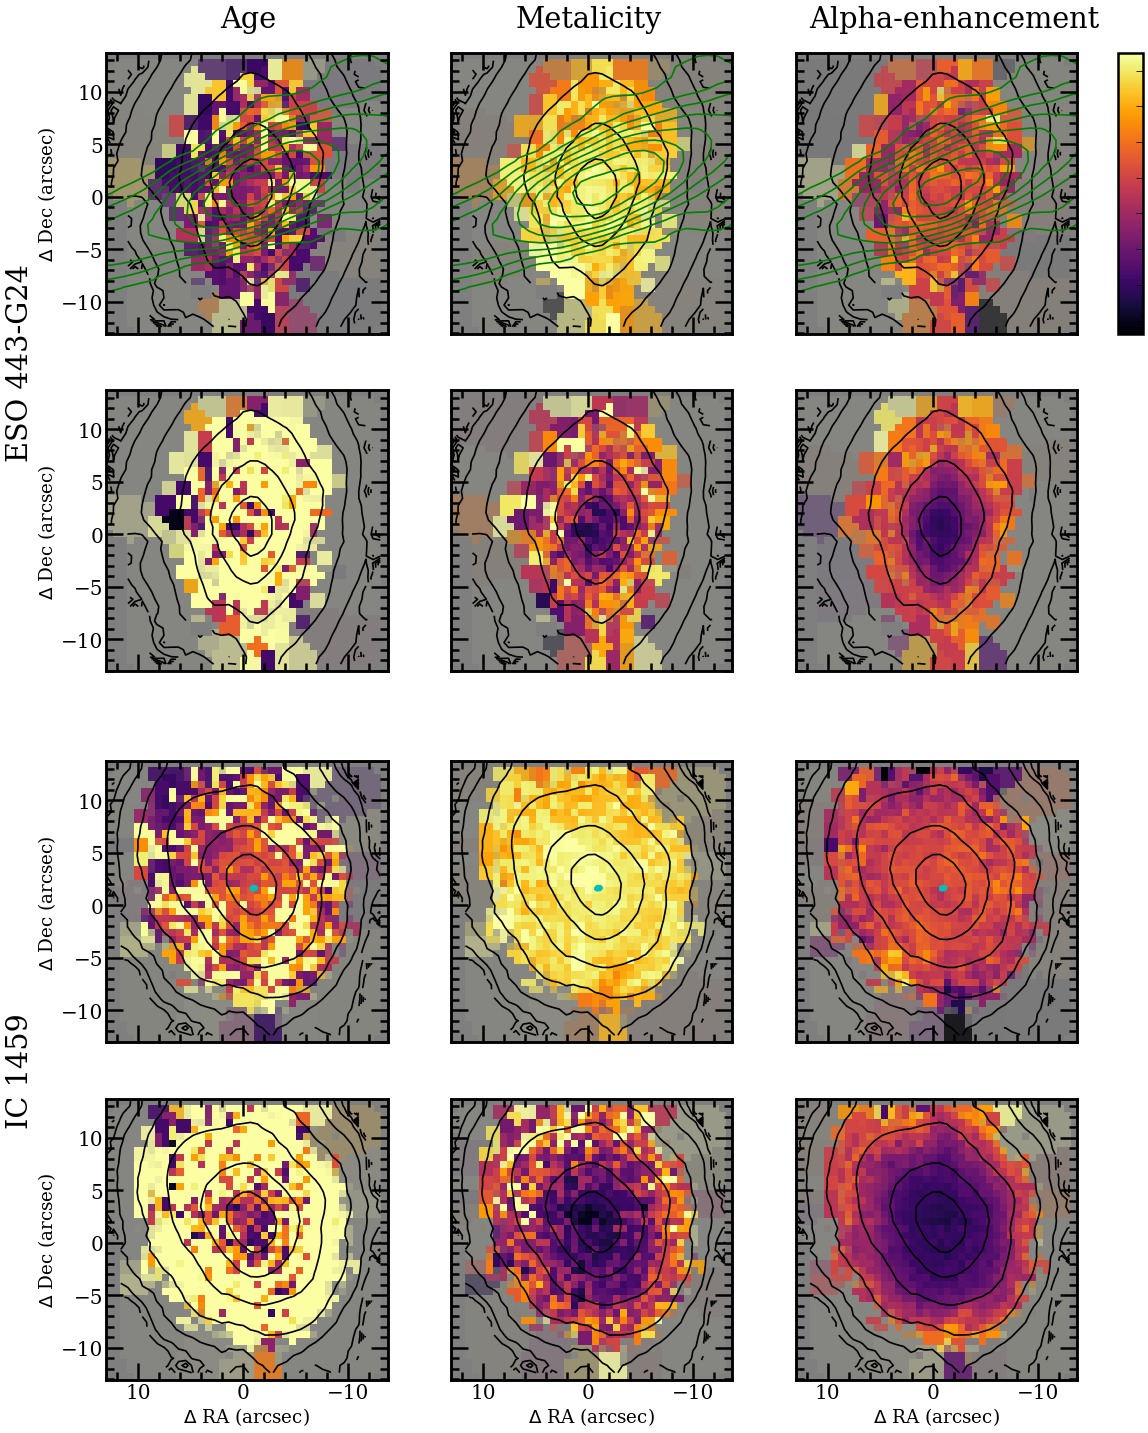
\includegraphics[height=0.63\textheight]{chapter4/vimos/pop1.png}
			\caption[VIMOS stellar population maps]{VIMOS stellar population maps: Left to right: age, metallicity and alpha enhancement; Top to bottom: ESO 443-G24 and IC 1459. Alternate rows show a given parameter its associated uncertainty. contours are as in Fig.\,\ref{fig:VIMOS_stellar}. Limits on the colour scale are: age (and associated uncertainty) 0--15 (0--2)\,Gyr, metallicity (and associated uncertainty) -2.25--0.67 (0--0.4)\,$\mathrm{dex}$ and alpha enhancement (and associated uncertainty) -0.3--0.5 (0-0.25)\,$\mathrm{dex}$.}
			\label{fig:VIMOS_pop}
		\end{figure}
		\begin{figure}
			\centering
			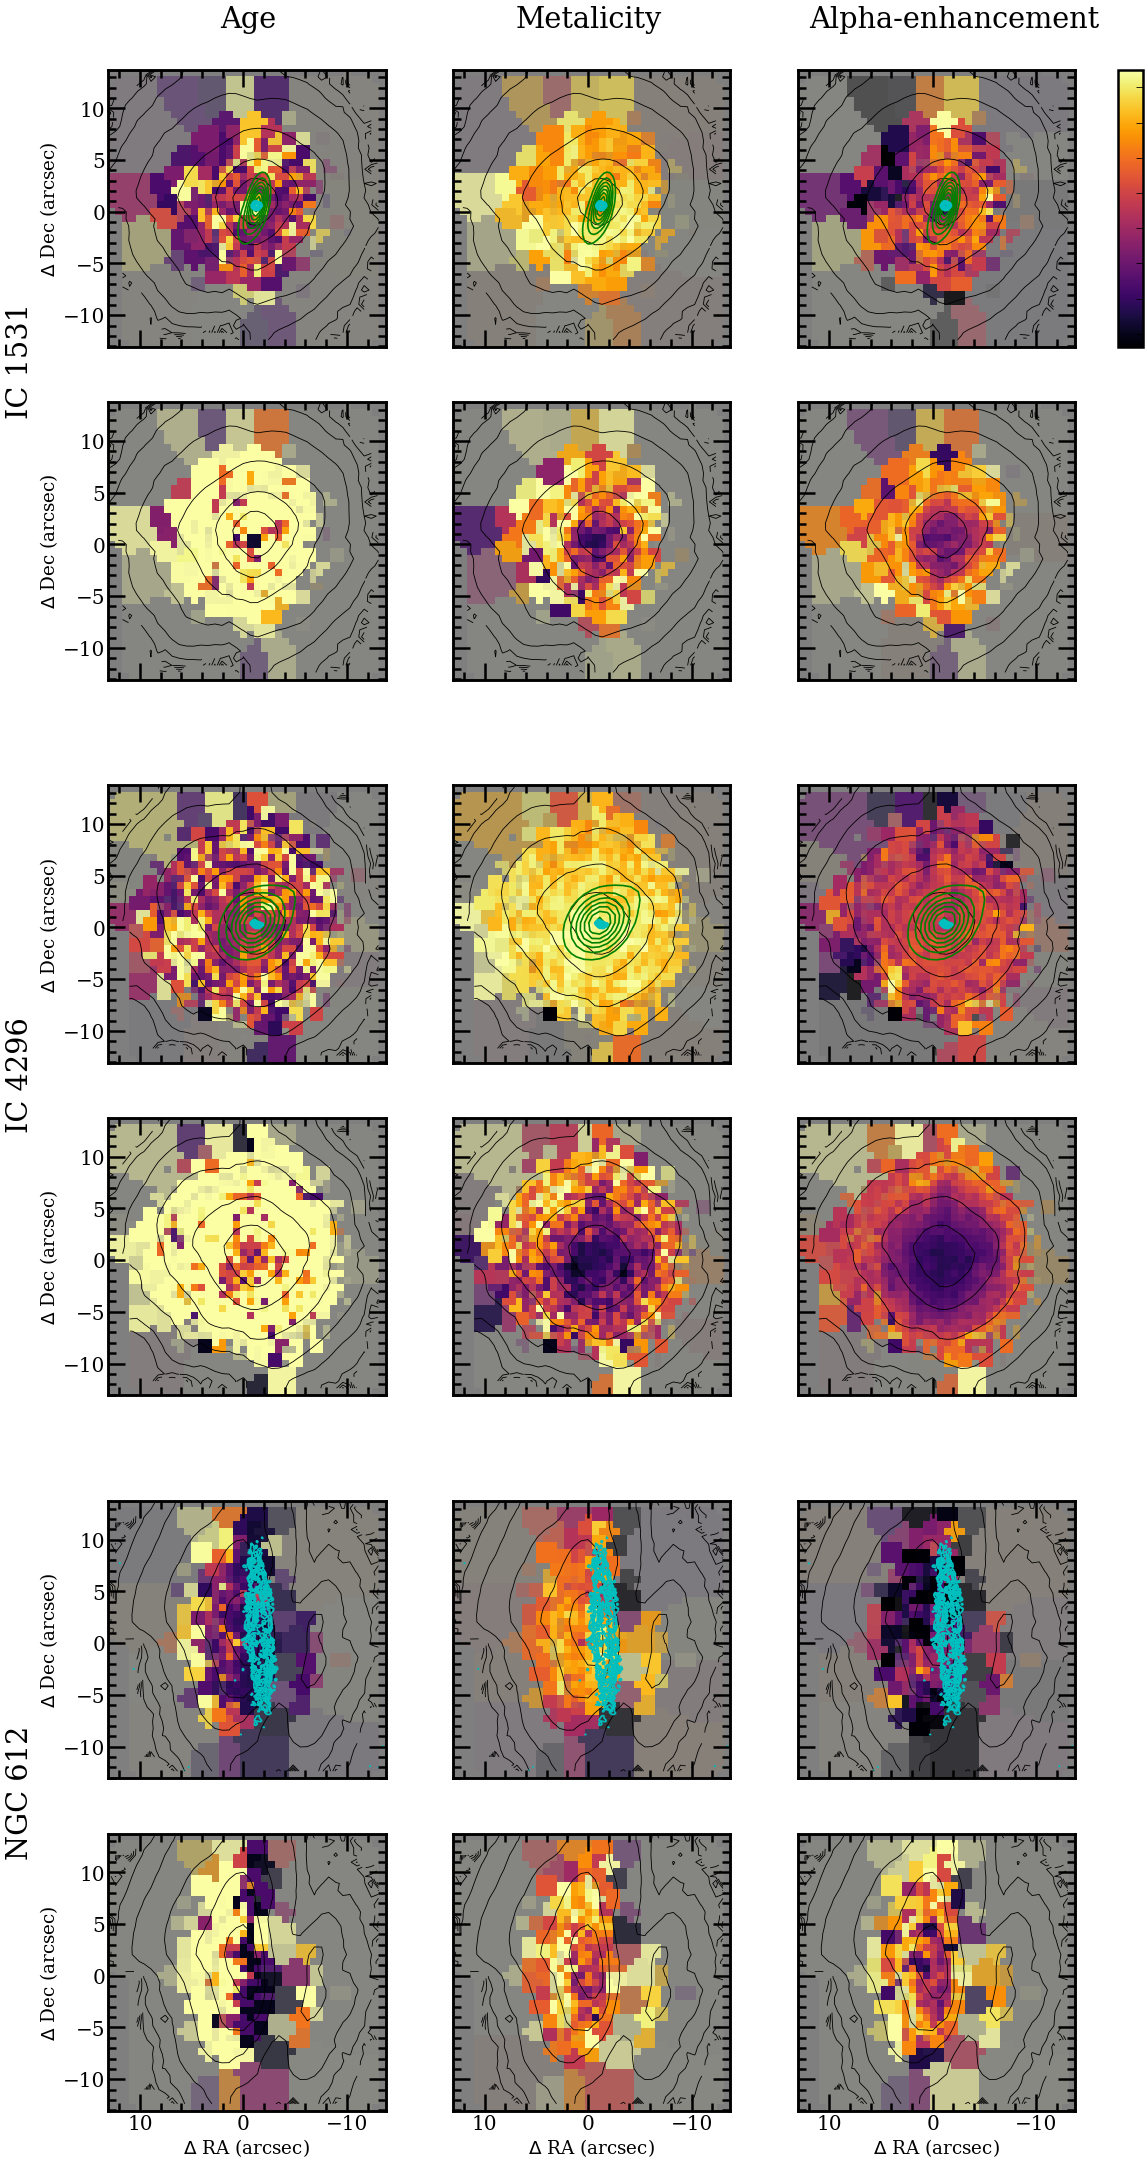
\includegraphics[height=0.94\textheight]{chapter4/vimos/pop2.png}
			\contcaption{\textit{Continued.}}% for IC 4296, NGC 612 and NGC 1399}
		\end{figure}
		\begin{figure}
			\centering
			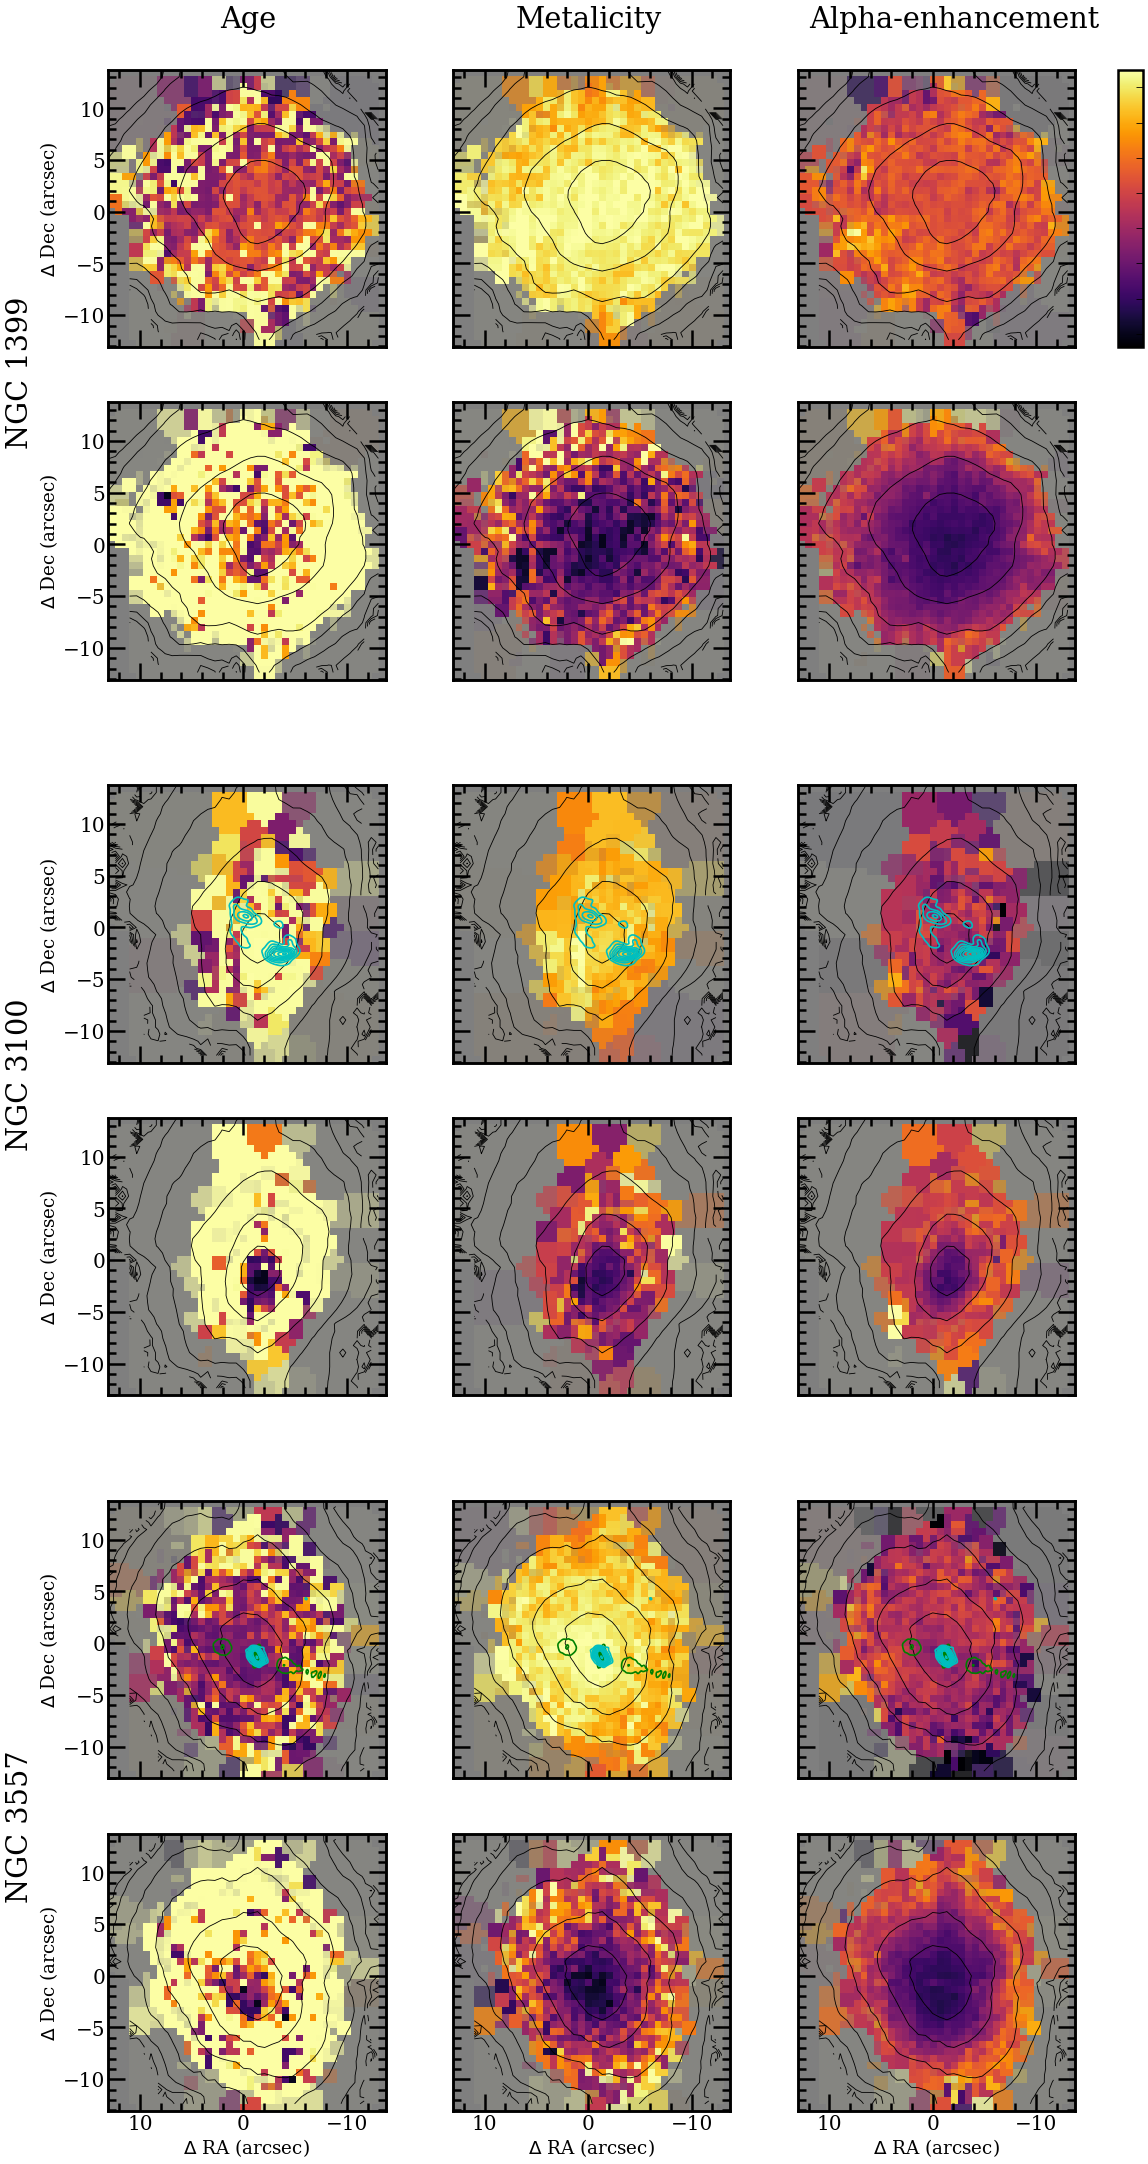
\includegraphics[height=0.94\textheight]{chapter4/vimos/pop3.png}
			\contcaption{\textit{Continued.}}% for NGC 3100, NGC 3557 and NGC 7075}
		\end{figure}
		\begin{figure}
			\centering
			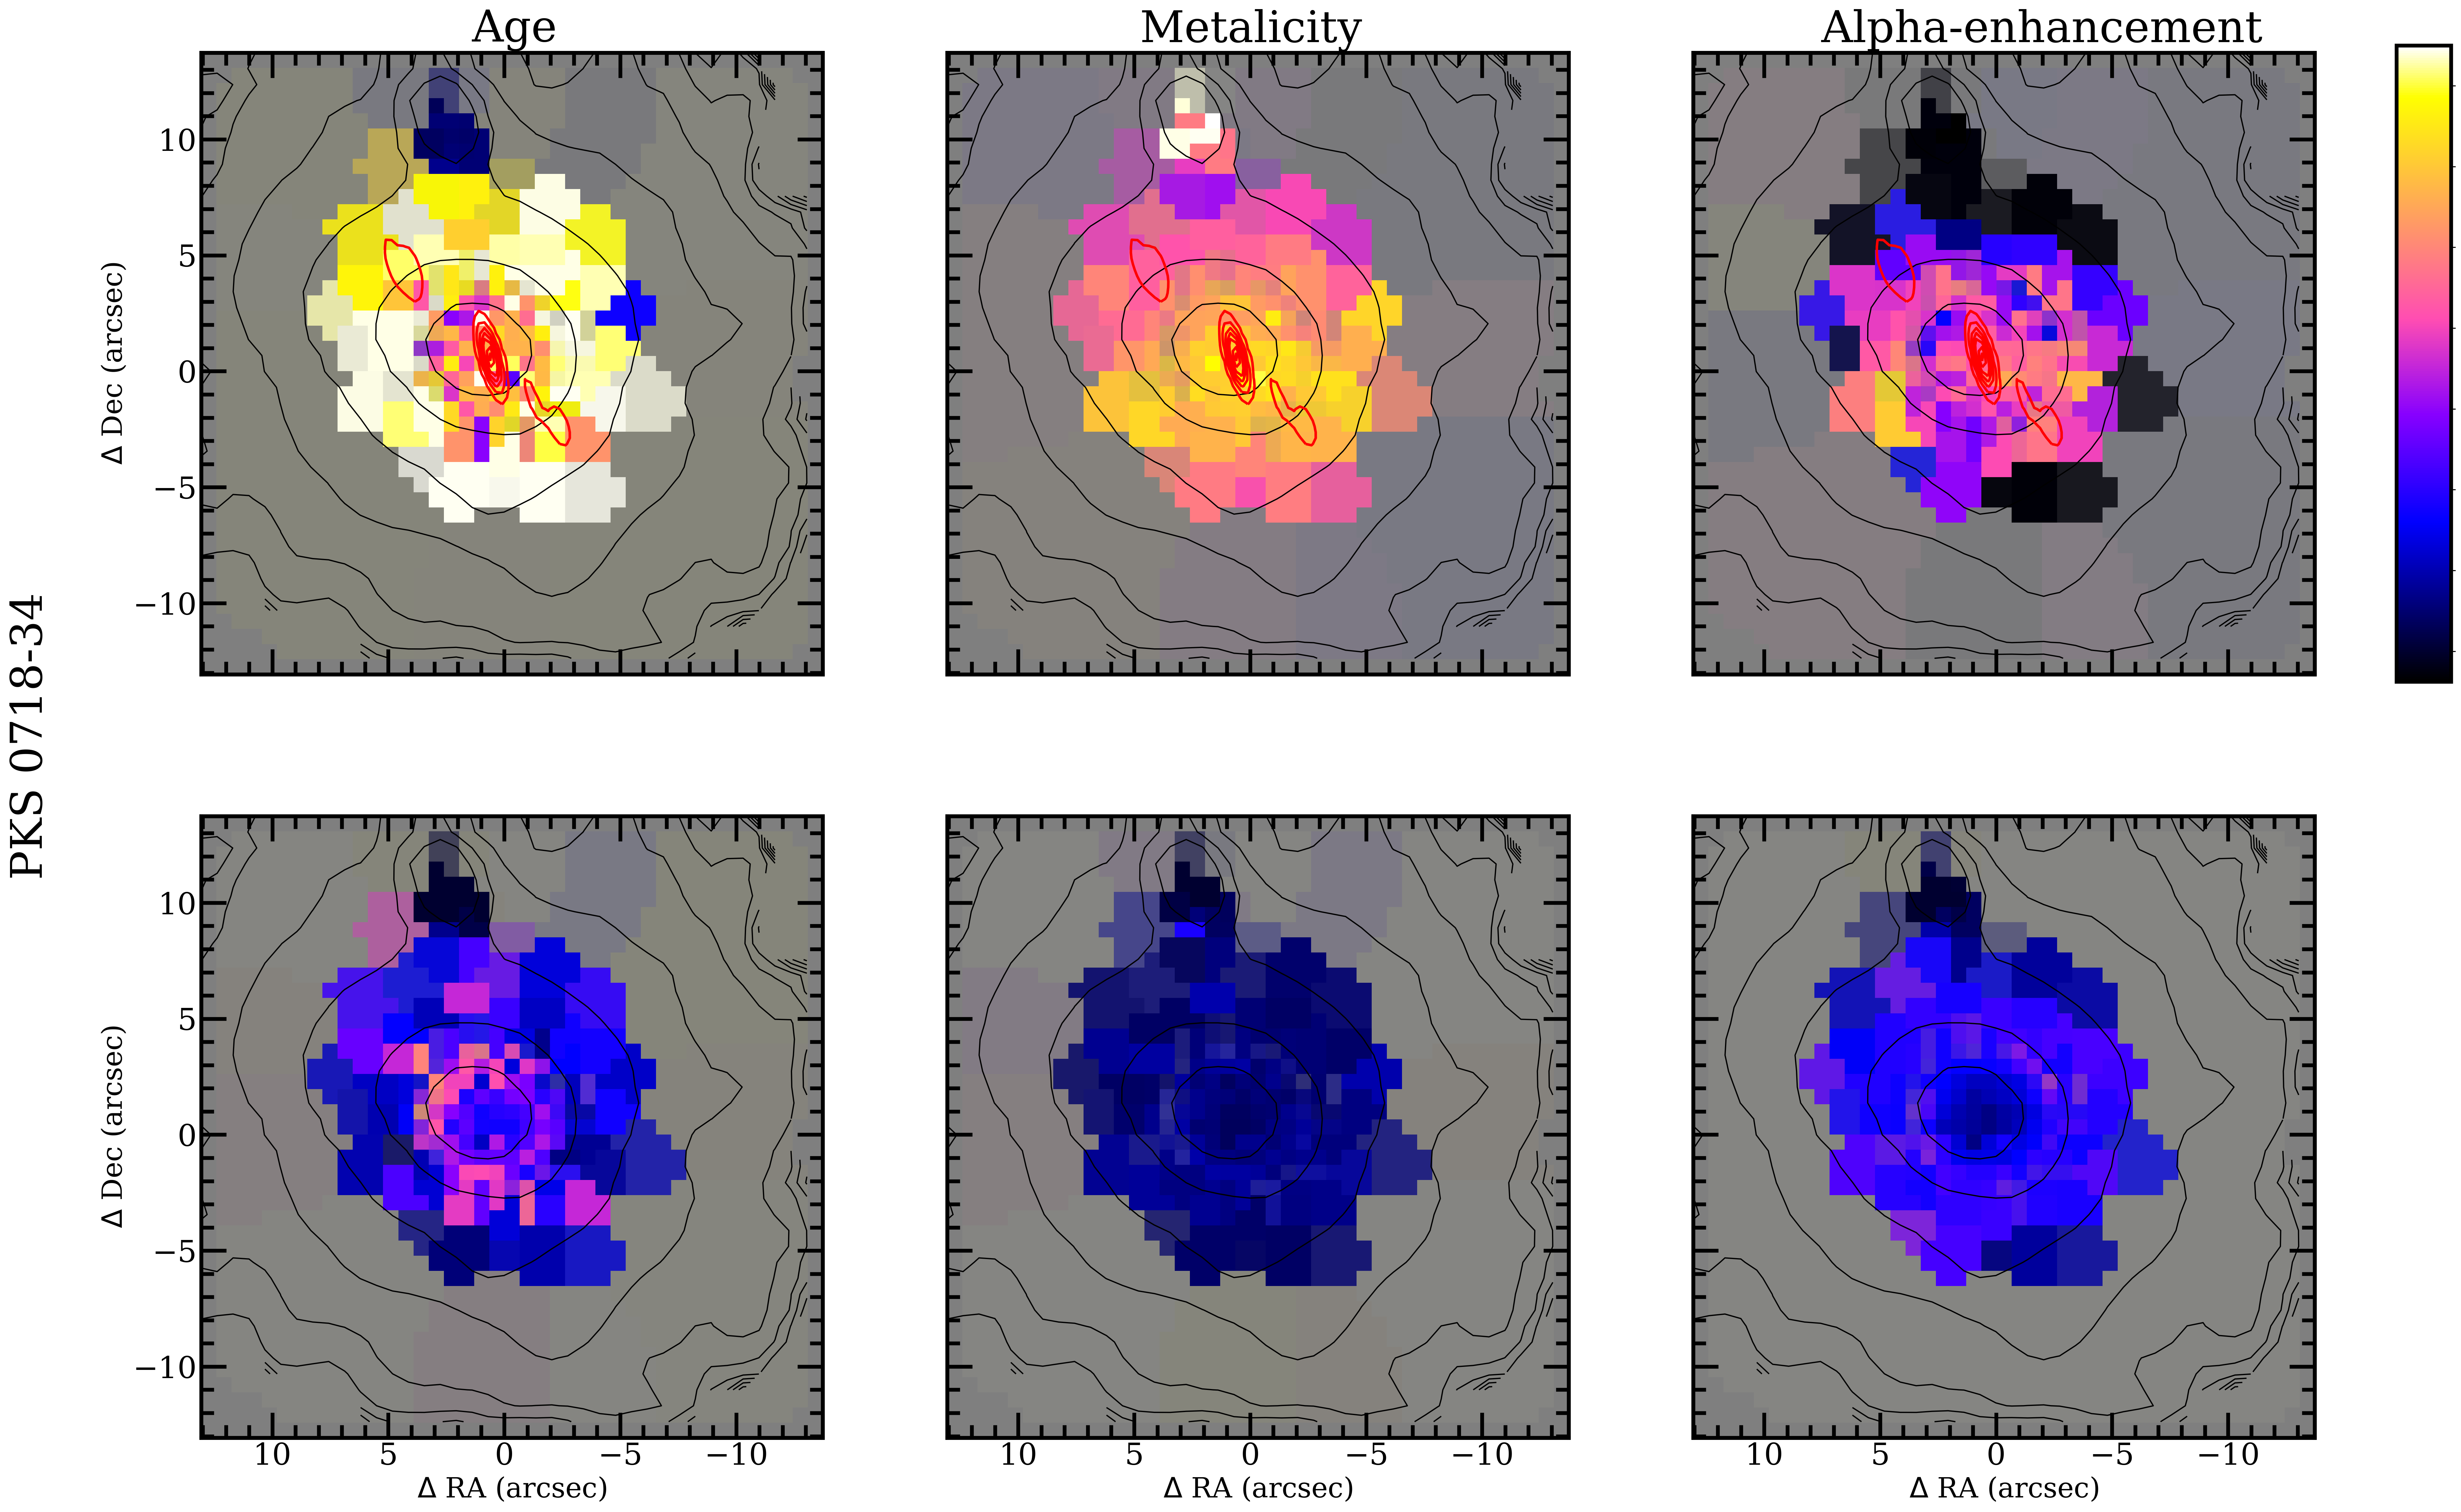
\includegraphics[height=0.63\textheight]{chapter4/vimos/pop4.png}
			\contcaption{\textit{Continued.}}% for PKS 718-34}
		\end{figure}

		\begin{figure}
			\centering
			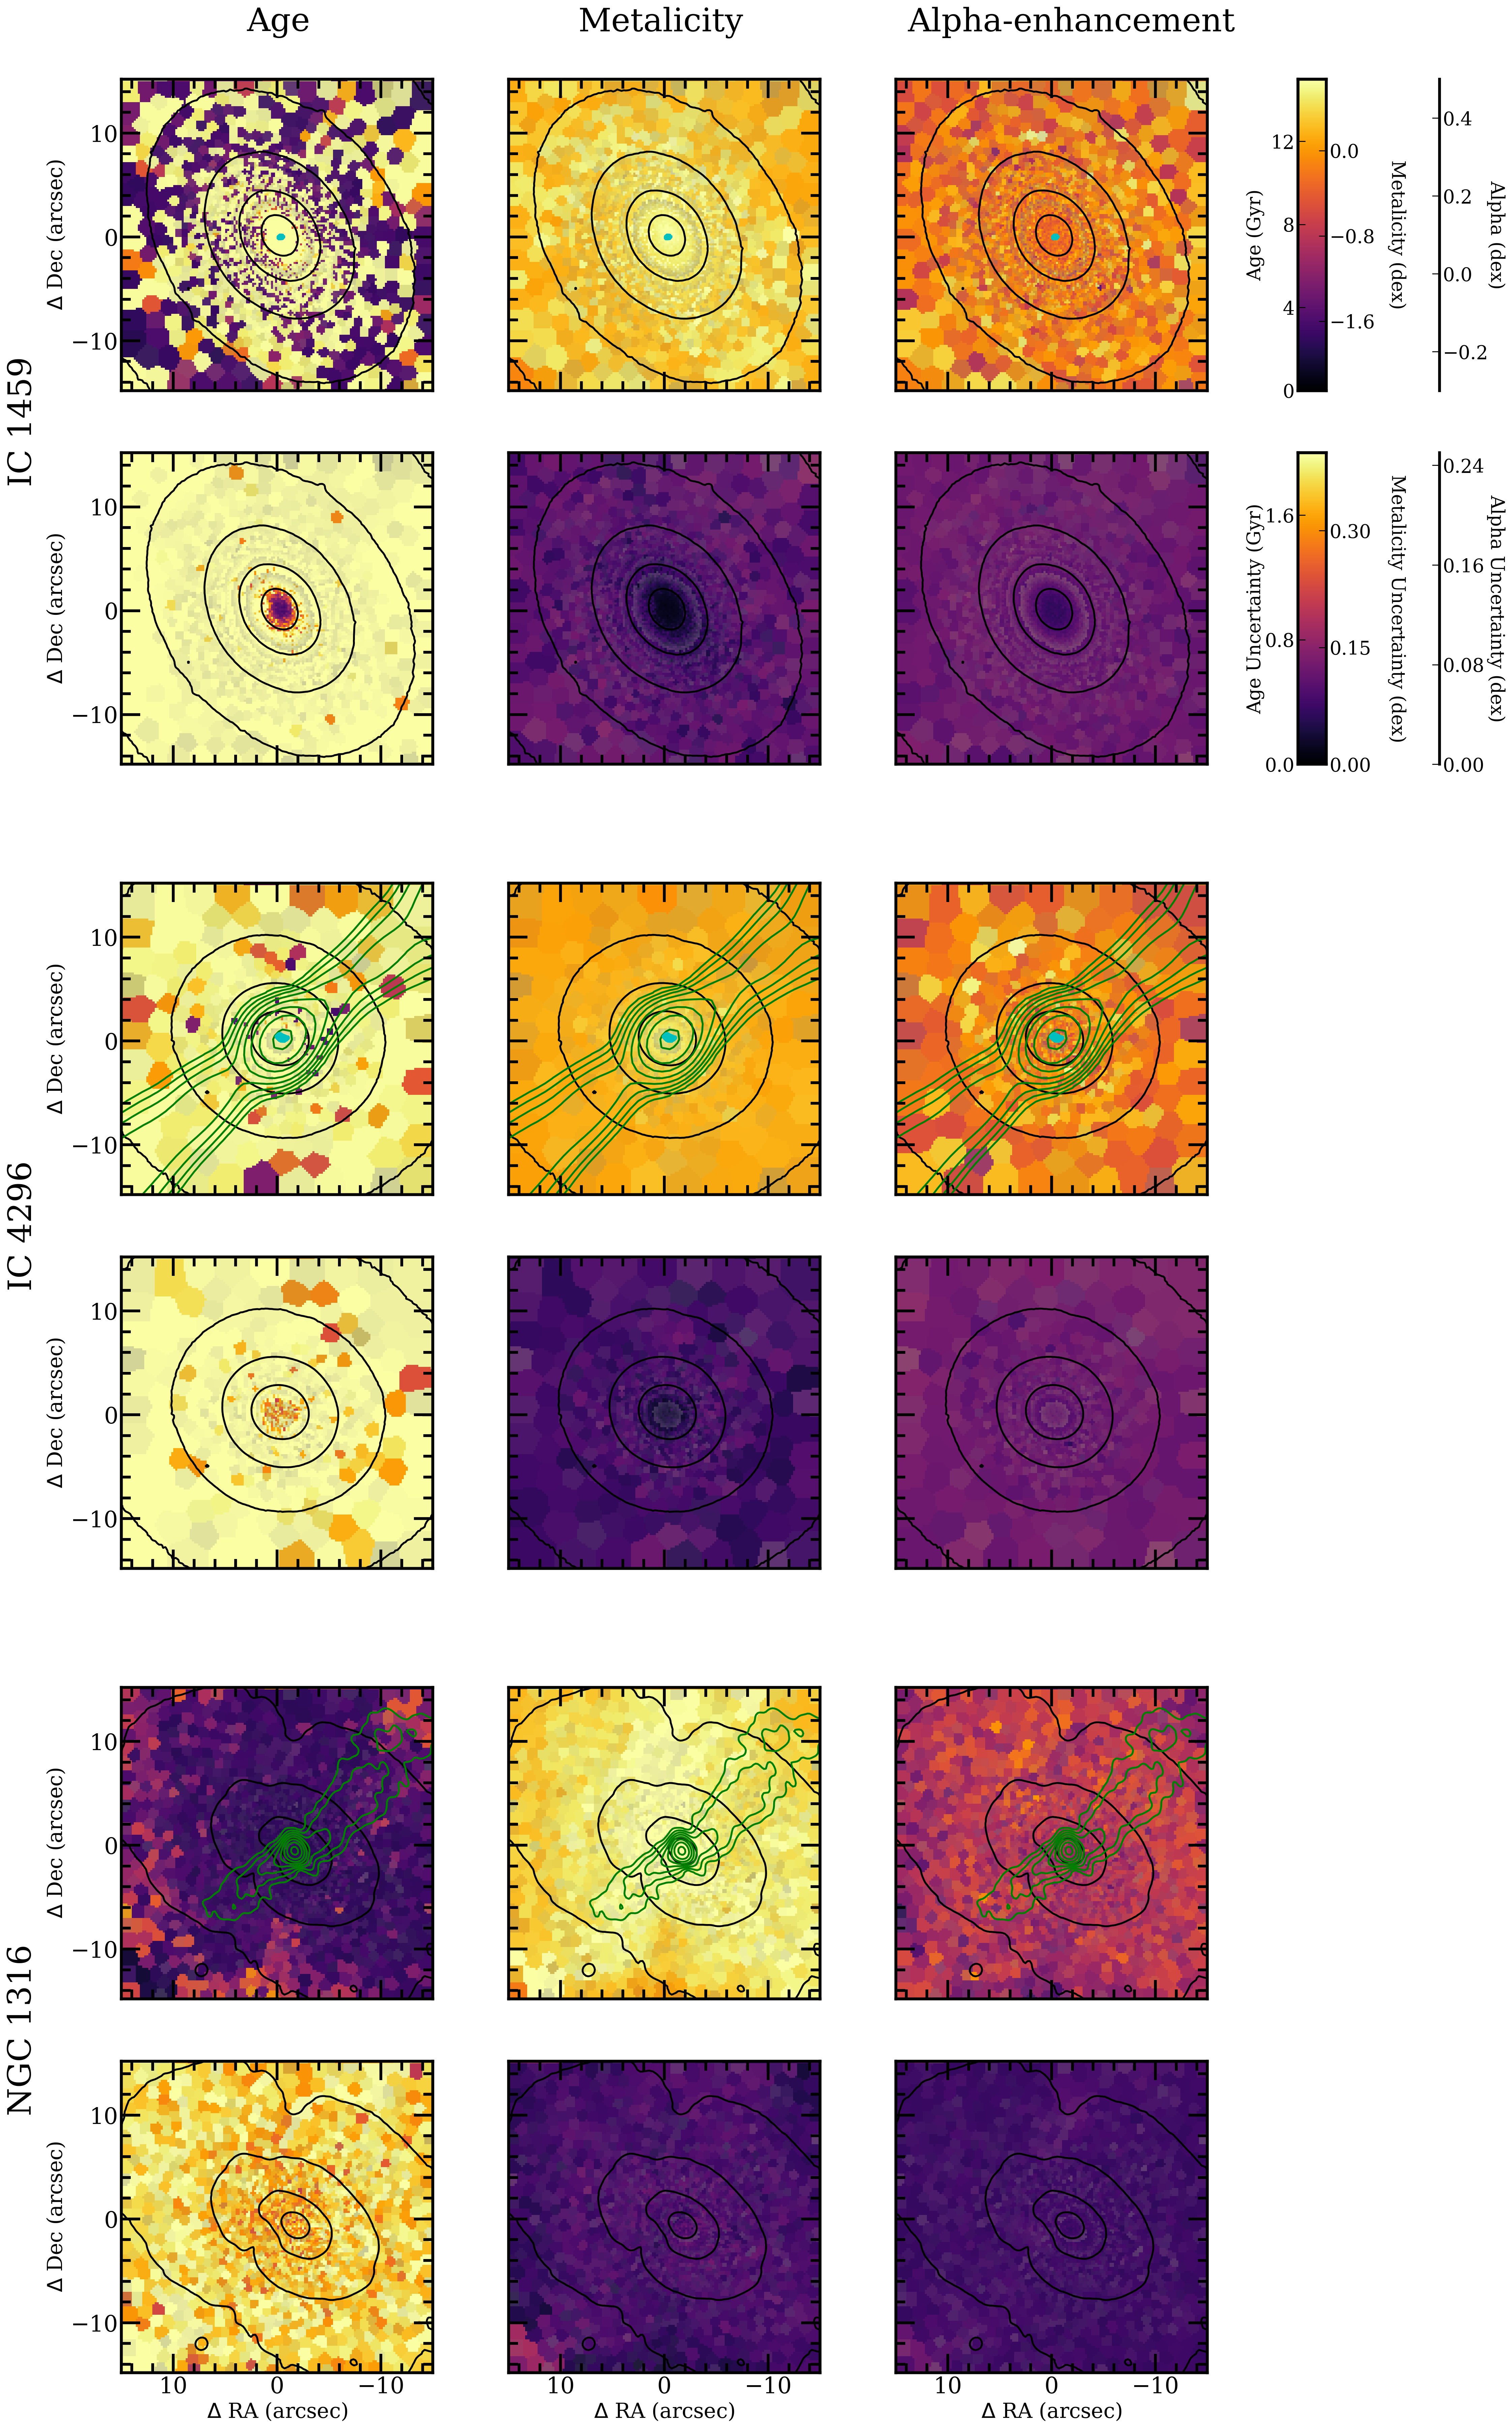
\includegraphics[height=0.94\textheight]{chapter4/muse/pop1.png}
			\caption[MUSE stellar population maps]{As in Figure \ref{fig:VIMOS_pop} but for the MUSE stellar population maps.}
			\label{fig:MUSE_pop}
		\end{figure}
		\begin{figure}
			\centering
			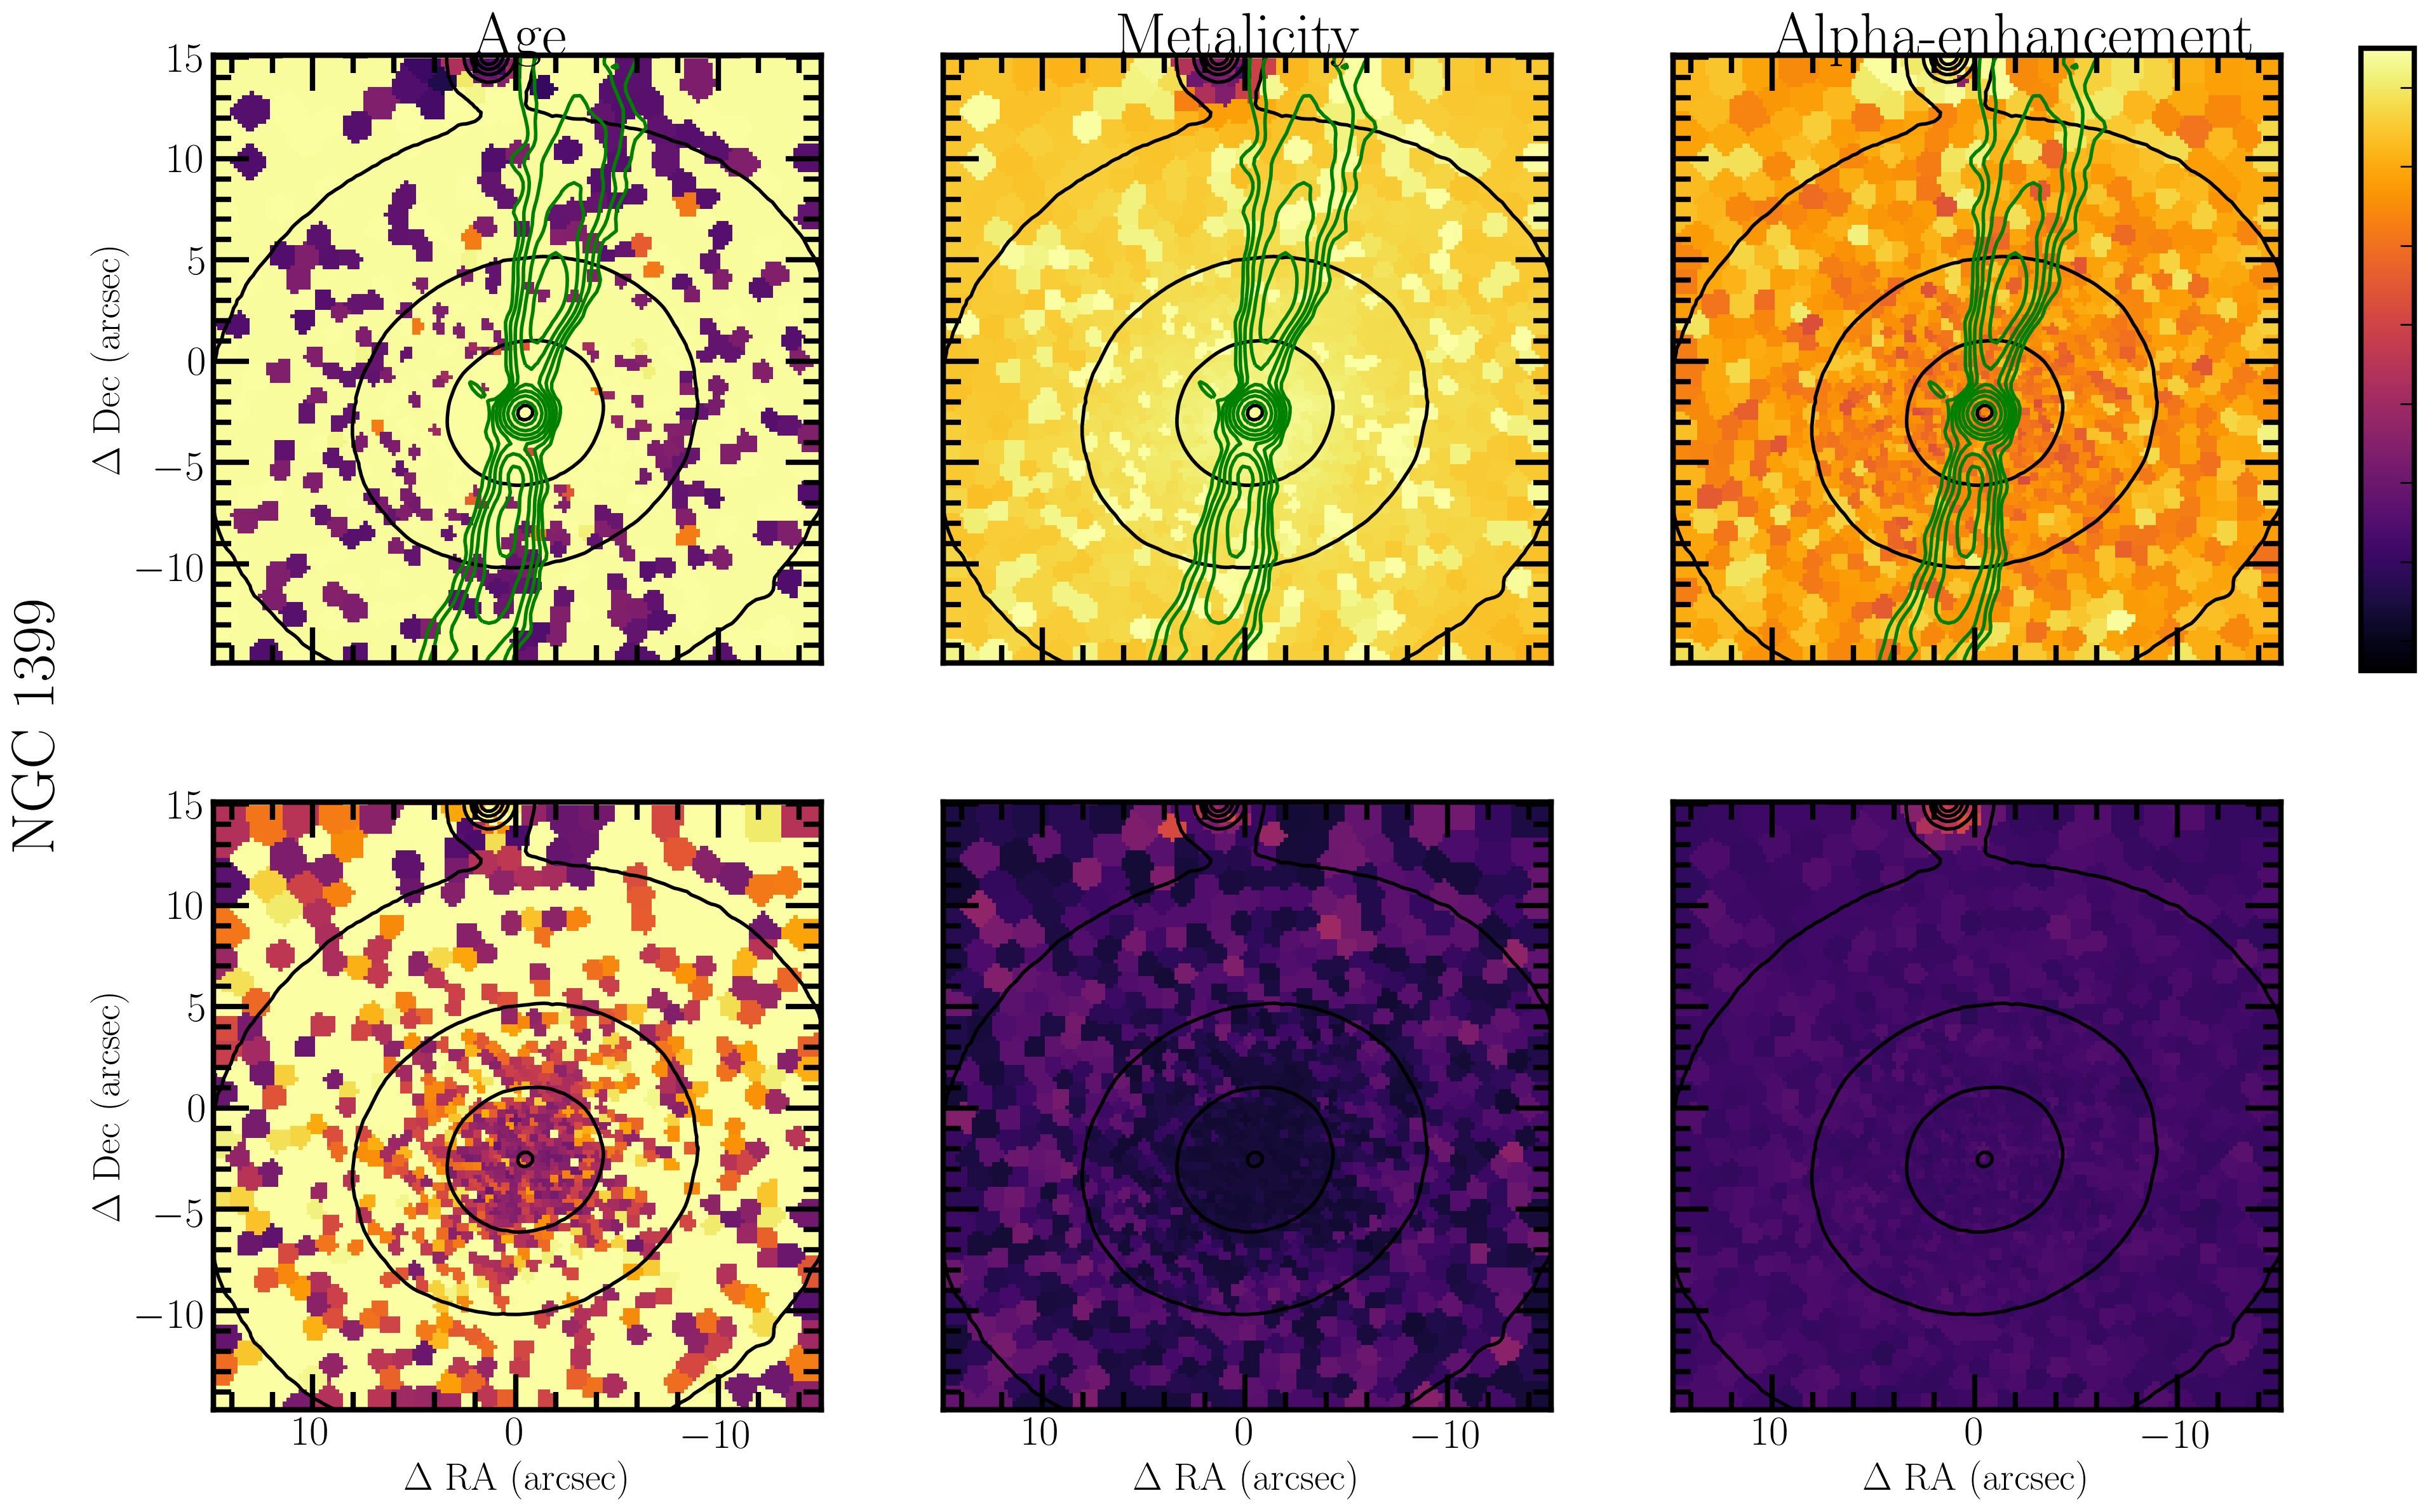
\includegraphics[height=0.31\textheight]{chapter4/muse/pop2.png}
			\contcaption{\textit{Continued.}}
		\end{figure}


		\subsubsection{Radial Gradients in Stellar Populations}
			\label{subsubsec:popGrad}

			\citet{Koleva2011} showed that while individual galaxies can have a wide range of radial gradients of age and metallicity, the mean gradient (within a mass bin) is approximately constant across a large mass range. They assume a linear relationship between $\log t$ or [Fe/H] and $\log (R/\mathrm{R_e})$. We repeat this fit with our Southern Sample with the results shown in Table \ref{tab:popGrad}. 

			\begin{table}
				\centering
				\caption{The radial gradients of the most-likely SSP models.}
				\label{tab:popGrad}
				\begin{tabular}{l c c c c}
					\hline
					\hline 
					Galaxy 	& \multicolumn{2}{c}{$\Delta_\text{log age}$} & \multicolumn{2}{c}{$\Delta_\text{[Fe/H]}$} \\
						& VIMOS & MUSE & VIMOS & MUSE
						% & dex\,arcsec$^{-1}$ & dex\,arcsec$^{-1}$ \\
					\hline
					ESO 443-G024 & $0.019 \pm 0.013$ & -- & $-0.01 \pm 0.02$ & -- \\
					IC 1459 	& $0.005 \pm 0.015$ & $0.003 \pm 0.002$ & $-0.02 \pm 0.02$ & $0.00 \pm 0.06$ \\
					IC 1531 	& $0.012 \pm 0.015$ & -- & $0.01 \pm 0.02$ & -- \\
					IC 4296		& $0.012 \pm 0.010$ & $0.000 \pm 0.002$ & $-0.03 \pm 0.01$ & $0.04 \pm 0.08$ \\
					NGC 612 	& $0.068 \pm 0.060$ & -- & $-0.11 \pm 0.02$ & -- \\
					NGC 1316 	& -- & $0.001 \pm 0.002$ & -- &$0.05 \pm 0.03$ \\
					NGC 1399 	& $0.019 \pm 0.005$ & $0.001 \pm 0.002$ & $-0.02 \pm 0.03$ & $0.10 \pm 0.09$ \\
					NGC 3100 	& $0.000 \pm 0.010$ & -- & $-0.06 \pm 0.01$ & -- \\
					NGC 3557 	& $0.048 \pm 0.039$ & -- & $-0.05 \pm 0.05$ & -- \\
					NGC 7075 	& $0.007 \pm 0.011$ & -- & $-0.07 \pm 0.02$ & -- \\
					PKS 718-34  & $0.002 \pm 0.009$ & -- & $-0.17 \pm 0.03$ & -- \\
					\hline
					\hline
				\end{tabular}
			\end{table}

			We find average gradients of $\Delta_\text{log age} = 0.014\pm0.007$% \,\mathrm{dex \, arcsec^{-1}}$
			 and $\Delta_\text{[Fe/H]} = -0.03\pm0.01$% \, \mathrm{dex \, arcsec^{-1}}$
			. This is consistent with \citet{Koleva2011} who, for elliptical galaxies found average gradients of $0.06\pm0.09$% \, \mathrm{dex \, arcsec^{-1}}$
			 and $-0.26\pm0.08$% \, \mathrm{dex \, arcsec^{-1}}$
			 for the age and metallicity gradients, respectively. For S0s they find flatter corresponding gradients of $0.01\pm0.11$%\, \mathrm{dex \, arcsec^{-1}}$
			 and $-0.12\pm0.13$%\, \mathrm{dex \, arcsec^{-1}}$
			. 

% SSP -- sigma relation here?



	\subsection{Kinematically-Decoupled Cores}
		\label{subsec:popKDC}

		\citet{Kuntschner2010} found that kinematically-decoupled cores (KDCs) exist in two classes: they are either small or contain an old stellar population. The size of the KDC is defined as the radius of the region surrounding the KDC where the superposition of the two components (the KDC and the host galaxy) results in a local minimum in the mean velocity. The age of the most-likely SSP model for the spatially integrated spectrum within an aperture 1\arcsec\ on the centre of the galaxy is taken as the KDC's age.

		The small KDCs tend to be found in fast rotators with galaxy-wide young stellar populations and still younger stellar populations within the KDC. They also tend to be counter-rotating or very close to counter-rotating with respect to the host galaxy (it is too difficult to distinguish the co-rotating KDCs that should be expected from their host galaxies). \citet{Kuntschner2010} suggests that the dominance of the stellar light of these KDCs over the other stars in the centre of the galaxies will reduce as time passes. As such, it is thought that old, small KDCs do exist, but they are not observable. \citet{Kuntschner2010} further propose that these KDCs are the result of gas accreted into the galaxy, settling into a counter-rotating disc near the centre of the galaxy, before forming the stars that make up the KDC. 

		The large KDCs are typically embedded in slow rotators. They have no upper limit on the age of their stellar populations suggesting that the stars within the KDC dominate in total mass as well as surface brightness. Thus, they do not fade into their host galaxies as they age unlike the small KDCs. \citet{Bois2011} showed major mergers may well result in such large KDCs if the initial spin axis of the progenitor galaxy with the lowest bulge-to-disc ratio (later-type) is anti-parallel to the orbital angular momentum vector. 

		In Fig.\,\ref{fig:KDC} we show the age and size of the 3 KDCs hosted by galaxies in our Southern sample. We include PKS 718-34 here but stress it is only tentatively classified as containing a KDC. As can be seen from Fig.\,\ref{fig:KDC}, PKS 718-34 would be an extremely large KDC, but is still consistent with the findings of \citet{Kuntschner2010}.

		\begin{figure}
			\centering
			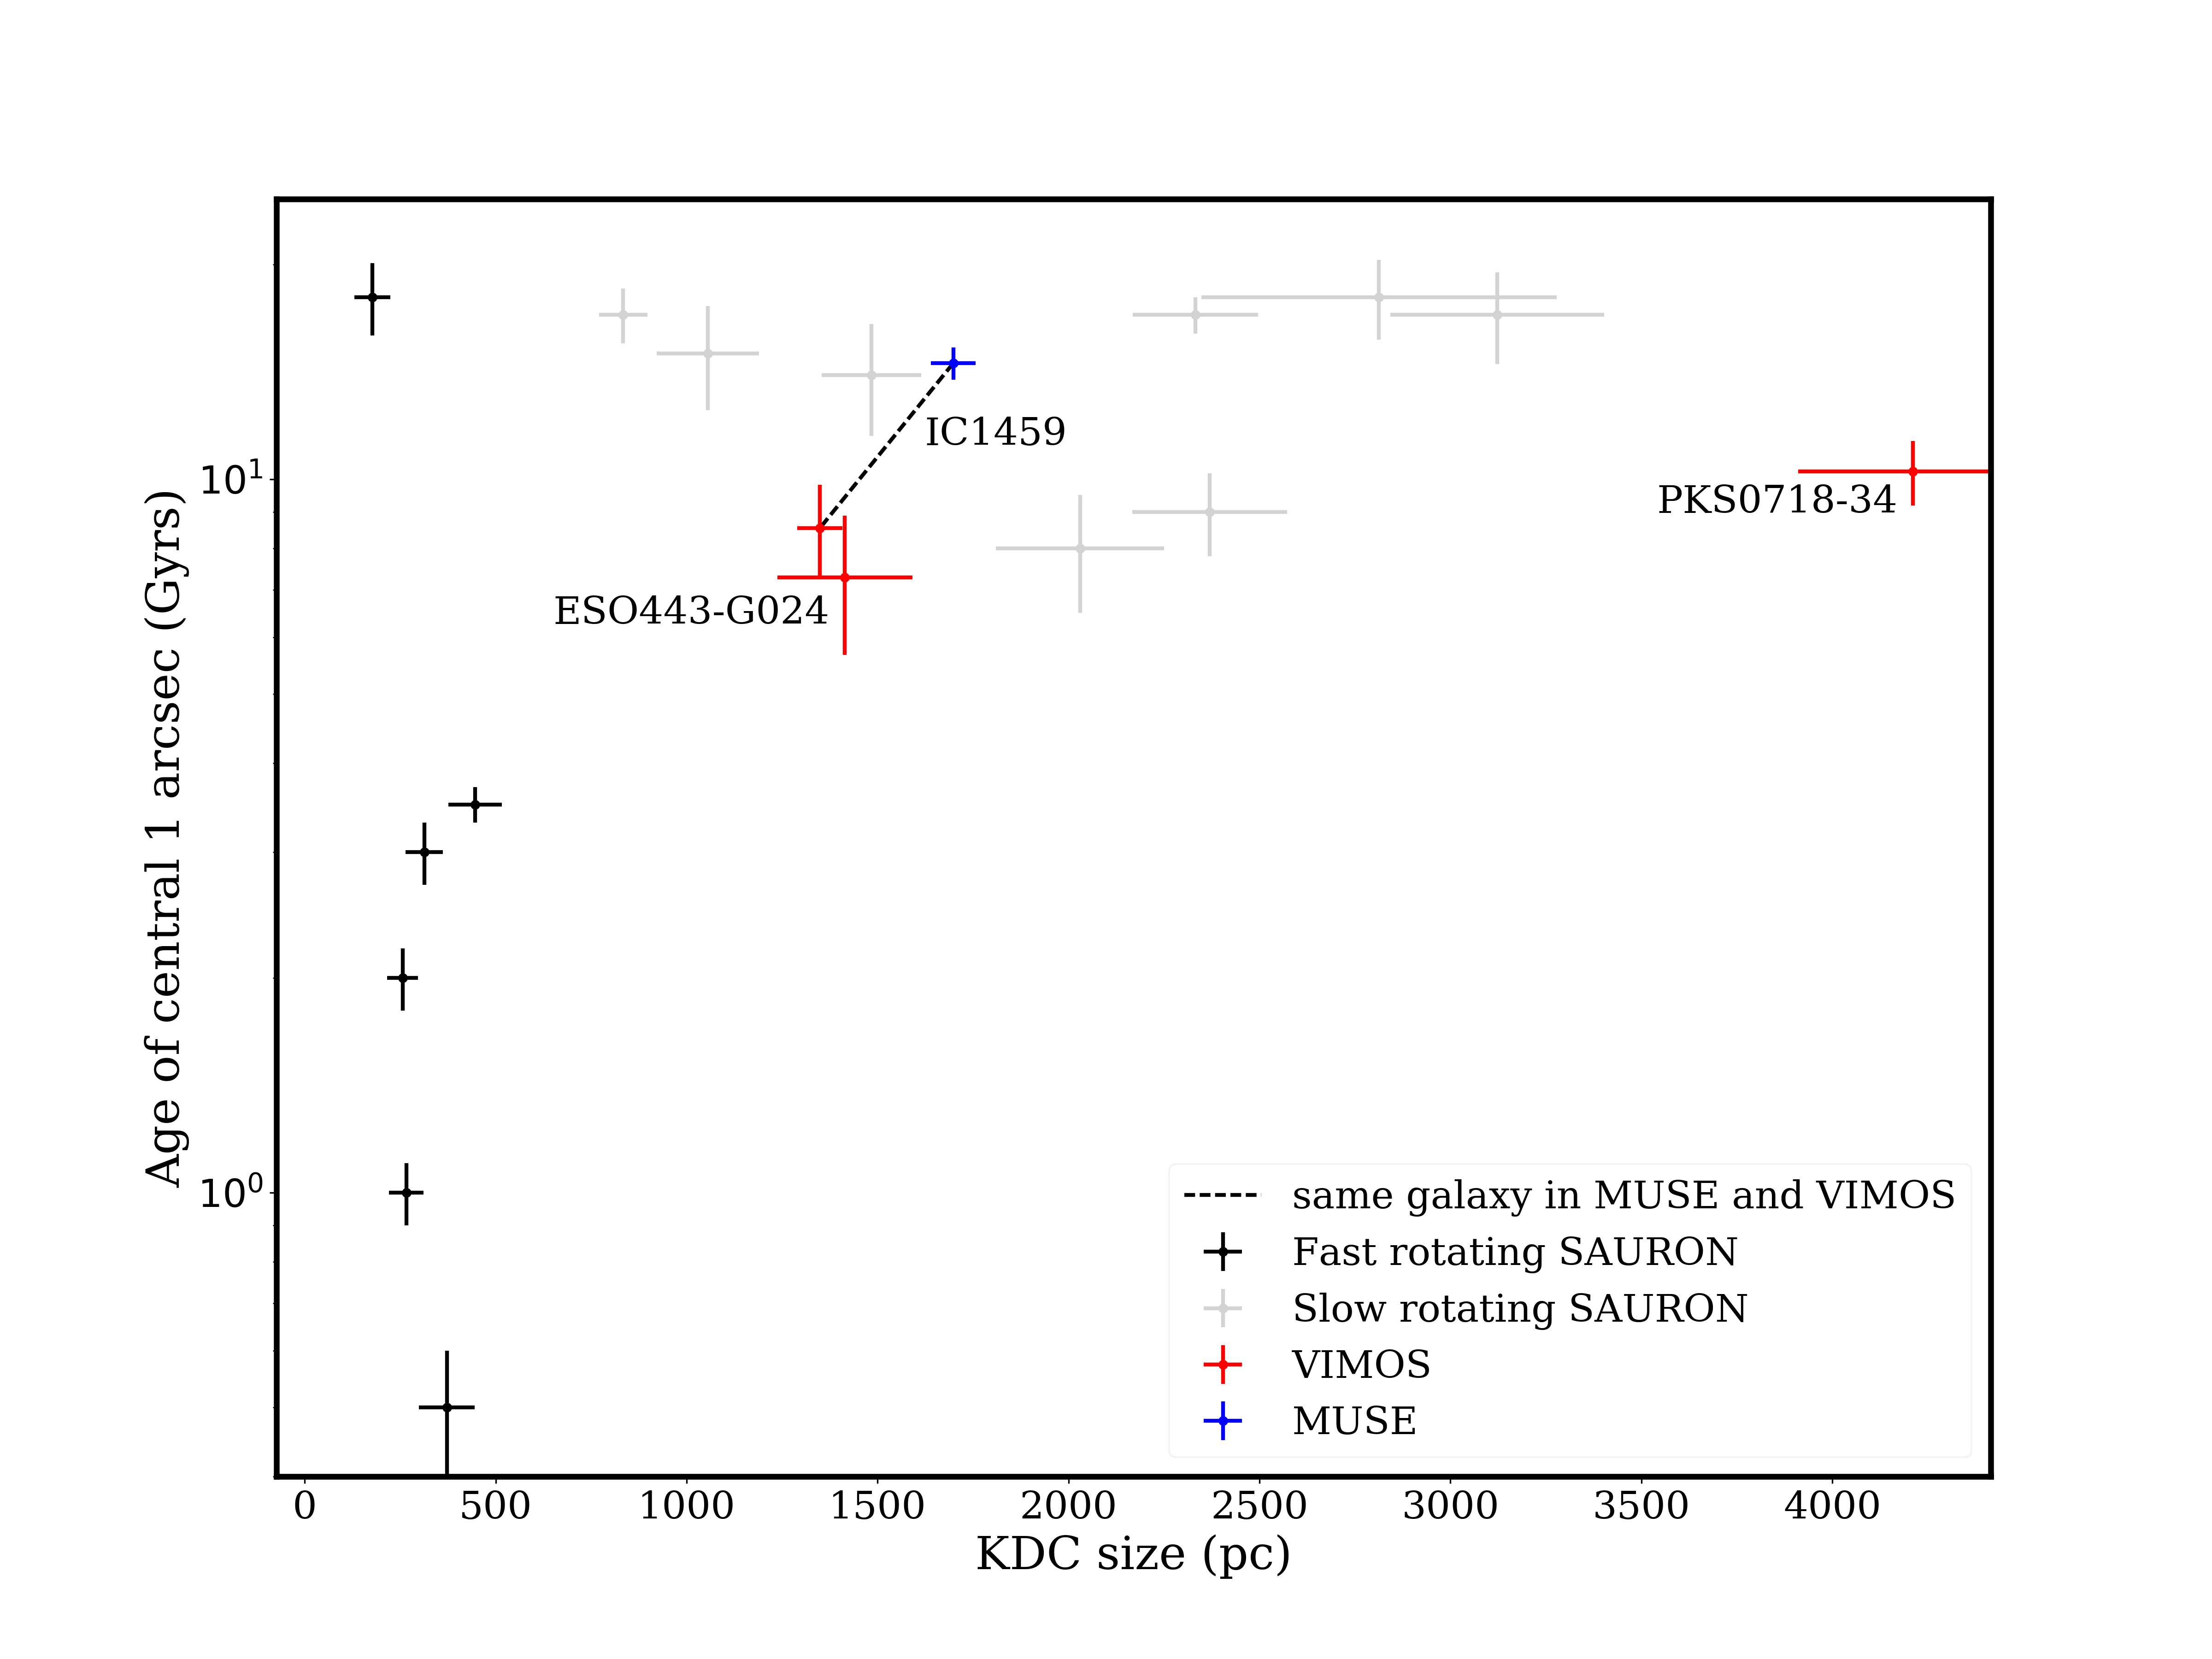
\includegraphics[width=.7\textwidth]{chapter4/KDC_size_age.png}
			\caption[KDC dichotomy]{The KDC size\,--\,age relation. KDCs exist in two classes: old and embedded in a slow rotator or small and embedded in a fast rotator. VIMOS observations are in red, MUSE in blue and SAURON from \citet{Kuntschner2010} in black and gray for fast and slow rotators respectively.}
			\label{fig:KDC}
		\end{figure}
	
\section{Discussion}
	\label{sec:stellarDiscussion}
	In this chapter we have shown that in terms of the stellar kinematic properties and stellar populations, our radio-selected Southern sample are no different to ordinary optically-selected ETGs. Our sample shows a mixture of of regularly- and non-regularly-rotating behaviours, with both classes showing evidence of consistency with observations of the intrinsic shapes of ordinary regular and non-regular rotators. At this stage we observe that 2 (with a tentative third) galaxies host large kinematically decoupled cores (KDCs). We also classify our sample galaxies into fast- and slow-rotators and find a consistent fraction ($45\pm13$\%) of slow-rotators to the ordinary ETG samples of the A+M sample, once the difference in the mass distribution between our Southern sample and the A+M sample are taken into account. 

	In terms of stellar populations, we find a remarkably similar gradient to the central Mg\,b verse stellar velocity dispersion relation to that of \citet{Ziegler1997}. Most of the galaxies in our Southern sample show typical ETG behavior: old, metal rich stellar populations, with a few exceptions: NGC 612 and NGC 1316 are both significantly younger than most ETGs and NGC 3557 has a young core. All are described in more detail in Appendix \ref{cha:Description}. We observe that all 3 KDCs contain old stellar populations and are consistent with being merger remnants. 

	All these observations and findings, are consistent with those of typical massive ETGs. This is consistent with the hypothesis that radio-galaxies are ordinary massive ETGs experiencing a normal but short-lived active phase. 

	Radio-loud lenticular (S0) galaxies are extremely rare with only a handful of known cases \citep[e.g.][]{Heckman1982, Morganti2011}, presumably due to the associated mass functions of both S0s and radio galaxies: both massive S0s and low-mass radio galaxies are rare, with a similar transition masses from rare to more numerous. NGC 612 is one of those rare cases.

	Finally, if molecular (cold) gas is the fuel source that is accreted on to the the central black holes of our Southern sample in order to power the radio jets, unless it is accreted in a highly turbulent fashion, it might be expected that some of that gas might form stars \citep[e.g.][]{Collin1999, Diamond-Stanic2012, LaMassa2013}. If this is the case then a young stellar population might be expected to dominate in the very central (1--2) spaxels. We our best-fitting age maps show no evidence of this. 